% Created 2020-05-27 三 21:12
% Intended LaTeX compiler: pdflatex
\documentclass[11pt]{article}
\usepackage[utf8]{inputenc}
\usepackage[T1]{fontenc}
\usepackage{graphicx}
\usepackage{grffile}
\usepackage{longtable}
\usepackage{wrapfig}
\usepackage{rotating}
\usepackage[normalem]{ulem}
\usepackage{amsmath}
\usepackage{textcomp}
\usepackage{amssymb}
\usepackage{capt-of}
\usepackage{imakeidx}
\usepackage{hyperref}
\usepackage{minted}
% TIPS
% \substack{a\\b} for multiple lines text





% pdfplots will load xolor automatically without option
\usepackage[dvipsnames]{xcolor}

\usepackage{forest}
% two-line text in node by [two \\ lines]
% \begin{forest} qtree, [..] \end{forest}
\forestset{
  qtree/.style={
    baseline,
    for tree={
      parent anchor=south,
      child anchor=north,
      align=center,
      inner sep=1pt,
    }}}
%\usepackage{flexisym}
% load order of mathtools and mathabx, otherwise conflict overbrace

\usepackage{mathtools}
%\usepackage{fourier}
\usepackage{pgfplots}
\usepackage{amsthm}
\usepackage{amsmath}
%\usepackage{unicode-math}
%
\usepackage{commath}
%\usepackage{,  , }
\usepackage{amsfonts}
\usepackage{amssymb}
% importing symbols https://tex.stackexchange.com/questions/14386/importing-a-single-symbol-from-a-different-font
%mathabx change every symbol
% use instead stmaryrd
%\usepackage{mathabx}
\usepackage{stmaryrd}
\usepackage{empheq}
\usepackage{tikz}
\usepackage{tikz-cd}
%\usepackage[notextcomp]{stix}
\usetikzlibrary{arrows.meta}
\usepackage[most]{tcolorbox}
%\utilde
%\usepackage{../../latexpackage/undertilde/undertilde}
% left and right superscript and subscript
\usepackage{actuarialsymbol}
\usepackage{threeparttable}
\usepackage{scalerel,stackengine}
\usepackage{stackrel}
% \stackrel[a]{b}{c}
\usepackage{dsfont}
% text font
\usepackage{newpxtext}
%\usepackage{newpxmath}

%\newcounter{dummy} \numberwithin{dummy}{section}
\newtheorem{dummy}{dummy}[section]
\theoremstyle{definition}
\newtheorem{definition}[dummy]{Definition}
\newtheorem{corollary}[dummy]{Corollary}
\newtheorem{lemma}[dummy]{Lemma}
\newtheorem{proposition}[dummy]{Proposition}
\newtheorem{theorem}[dummy]{Theorem}
\theoremstyle{definition}
\newtheorem{example}[dummy]{Example}
\theoremstyle{remark}
\newtheorem*{remark}{Remark}


\newcommand\what[1]{\ThisStyle{%
    \setbox0=\hbox{$\SavedStyle#1$}%
    \stackengine{-1.0\ht0+.5pt}{$\SavedStyle#1$}{%
      \stretchto{\scaleto{\SavedStyle\mkern.15mu\char'136}{2.6\wd0}}{1.4\ht0}%
    }{O}{c}{F}{T}{S}%
  }
}

\newcommand\wtilde[1]{\ThisStyle{%
    \setbox0=\hbox{$\SavedStyle#1$}%
    \stackengine{-.1\LMpt}{$\SavedStyle#1$}{%
      \stretchto{\scaleto{\SavedStyle\mkern.2mu\AC}{.5150\wd0}}{.6\ht0}%
    }{O}{c}{F}{T}{S}%
  }
}

\newcommand\wbar[1]{\ThisStyle{%
    \setbox0=\hbox{$\SavedStyle#1$}%
    \stackengine{.5pt+\LMpt}{$\SavedStyle#1$}{%
      \rule{\wd0}{\dimexpr.3\LMpt+.3pt}%
    }{O}{c}{F}{T}{S}%
  }
}

\newcommand{\bl}[1] {\boldsymbol{#1}}
\newcommand{\Wt}[1] {\stackrel{\sim}{\smash{#1}\rule{0pt}{1.1ex}}}
\newcommand{\wt}[1] {\widetilde{#1}}
\newcommand{\tf}[1] {\textbf{#1}}


%For boxed texts in align, use Aboxed{}
%otherwise use boxed{}

\DeclareMathSymbol{\widehatsym}{\mathord}{largesymbols}{"62}
\newcommand\lowerwidehatsym{%
  \text{\smash{\raisebox{-1.3ex}{%
    $\widehatsym$}}}}
\newcommand\fixwidehat[1]{%
  \mathchoice
    {\accentset{\displaystyle\lowerwidehatsym}{#1}}
    {\accentset{\textstyle\lowerwidehatsym}{#1}}
    {\accentset{\scriptstyle\lowerwidehatsym}{#1}}
    {\accentset{\scriptscriptstyle\lowerwidehatsym}{#1}}
}

\usepackage{graphicx}
    
% text on arrow for xRightarrow
\makeatletter
%\newcommand{\xRightarrow}[2][]{\ext@arrow 0359\Rightarrowfill@{#1}{#2}}
\makeatother


\newcommand{\dom}[1]{%
\mathrm{dom}{(#1)}
}

% Roman numerals
\makeatletter
\newcommand*{\rom}[1]{\expandafter\@slowromancap\romannumeral #1@}
\makeatother

\def \fR {\mathfrak{R}}
\def \bx {\boldsymbol{x}}
\def \bz {\boldsymbol{z}}
\def \ba {\boldsymbol{a}}
\def \bh {\boldsymbol{h}}
\def \bo {\boldsymbol{o}}
\def \bU {\boldsymbol{U}}
\def \bc {\boldsymbol{c}}
\def \bV {\boldsymbol{V}}
\def \bI {\boldsymbol{I}}
\def \bK {\boldsymbol{K}}
\def \bt {\boldsymbol{t}}
\def \bb {\boldsymbol{b}}
\def \bA {\boldsymbol{A}}
\def \bX {\boldsymbol{X}}
\def \bu {\boldsymbol{u}}
\def \bS {\boldsymbol{S}}
\def \bZ {\boldsymbol{Z}}
\def \bz {\boldsymbol{z}}
\def \by {\boldsymbol{y}}
\def \bw {\boldsymbol{w}}
\def \bT {\boldsymbol{T}}
\def \bF {\boldsymbol{F}}
\def \bS {\boldsymbol{S}}
\def \bm {\boldsymbol{m}}
\def \bW {\boldsymbol{W}}
\def \bR {\boldsymbol{R}}
\def \bQ {\boldsymbol{Q}}
\def \bS {\boldsymbol{S}}
\def \bP {\boldsymbol{P}}
\def \bT {\boldsymbol{T}}
\def \bY {\boldsymbol{Y}}
\def \bH {\boldsymbol{H}}
\def \bB {\boldsymbol{B}}
\def \blambda {\boldsymbol{\lambda}}
\def \bPhi {\boldsymbol{\Phi}}
\def \btheta {\boldsymbol{\theta}}
\def \bTheta {\boldsymbol{\Theta}}
\def \bmu {\boldsymbol{\mu}}
\def \bphi {\boldsymbol{\phi}}
\def \bSigma {\boldsymbol{\Sigma}}
\def \lb {\left\{}
\def \rb {\right\}}
\def \la {\langle}
\def \ra {\rangle}
\def \caln {\mathcal{N}}
\def \dissum {\displaystyle\Sigma}
\def \dispro {\displaystyle\prod}
\def \E {\mathbb{E}}
\def \Q {\mathbb{Q}}
\def \N {\mathbb{N}}
\def \V {\mathbb{V}}
\def \R {\mathbb{R}}
\def \P {\mathbb{P}}
\def \A {\mathbb{A}}
\def \Z {\mathbb{Z}}
\def \I {\mathbb{I}}
\def \C {\mathbb{C}}
\def \cala {\mathcal{A}}
\def \calb {\mathcal{B}}
\def \calq {\mathcal{Q}}
\def \calp {\mathcal{P}}
\def \cals {\mathcal{S}}
\def \calg {\mathcal{G}}
\def \caln {\mathcal{N}}
\def \calr {\mathcal{R}}
\def \calm {\mathcal{M}}
\def \calc {\mathcal{C}}
\def \calf {\mathcal{F}}
\def \calk {\mathcal{K}}
\def \call {\mathcal{L}}
\def \calu {\mathcal{U}}
\def \bcup {\bigcup}


\def \uin {\underline{\in}}
\def \oin {\overline{\in}}
\def \uR {\underline{R}}
\def \oR {\overline{R}}
\def \uP {\underline{P}}
\def \oP {\overline{P}}

\def \Ra {\Rightarrow}

\def \e {\enspace}

\def \sgn {\operatorname{sgn}}
\def \gen {\operatorname{gen}}
\def \ker {\operatorname{ker}}
\def \im {\operatorname{im}}

\def \tril {\triangleleft}

% \varprod
\DeclareSymbolFont{largesymbolsA}{U}{txexa}{m}{n}
\DeclareMathSymbol{\varprod}{\mathop}{largesymbolsA}{16}

% \bigtimes
\DeclareFontFamily{U}{mathx}{\hyphenchar\font45}
\DeclareFontShape{U}{mathx}{m}{n}{
      <5> <6> <7> <8> <9> <10>
      <10.95> <12> <14.4> <17.28> <20.74> <24.88>
      mathx10
      }{}
\DeclareSymbolFont{mathx}{U}{mathx}{m}{n}
\DeclareMathSymbol{\bigtimes}{1}{mathx}{"91}
% \odiv
\DeclareFontFamily{U}{matha}{\hyphenchar\font45}
\DeclareFontShape{U}{matha}{m}{n}{
      <5> <6> <7> <8> <9> <10> gen * matha
      <10.95> matha10 <12> <14.4> <17.28> <20.74> <24.88> matha12
      }{}
\DeclareSymbolFont{matha}{U}{matha}{m}{n}
\DeclareMathSymbol{\odiv}         {2}{matha}{"63}


\newcommand\subsetsim{\mathrel{%
  \ooalign{\raise0.2ex\hbox{\scalebox{0.9}{$\subset$}}\cr\hidewidth\raise-0.85ex\hbox{\scalebox{0.9}{$\sim$}}\hidewidth\cr}}}
\newcommand\simsubset{\mathrel{%
  \ooalign{\raise-0.2ex\hbox{\scalebox{0.9}{$\subset$}}\cr\hidewidth\raise0.75ex\hbox{\scalebox{0.9}{$\sim$}}\hidewidth\cr}}}

\newcommand\simsubsetsim{\mathrel{%
  \ooalign{\raise0ex\hbox{\scalebox{0.8}{$\subset$}}\cr\hidewidth\raise1ex\hbox{\scalebox{0.75}{$\sim$}}\hidewidth\cr\raise-0.95ex\hbox{\scalebox{0.8}{$\sim$}}\cr\hidewidth}}}
\newcommand{\stcomp}[1]{{#1}^{\mathsf{c}}}


\setcounter{secnumdepth}{2}
\setcounter{tocdepth}{2}
\DeclareMathOperator{\Frac}{Frac}
\author{Joseph J. Rotman}
\date{\today}
\title{\zallman Advanced Modern Algebra}
\hypersetup{
 pdfauthor={Joseph J. Rotman},
 pdftitle={\zallman Advanced Modern Algebra},
 pdfkeywords={},
 pdfsubject={},
 pdfcreator={Emacs 26.3 (Org mode 9.3.6)}, 
 pdflang={English}}
\begin{document}

\maketitle \clearpage
\setcounter{tocdepth}{2}
\tableofcontents \clearpage

\section{Things Past}
\label{sec:org6c7c66b}
\subsection{Some Number Theory}
\label{sec:org81cf445}
\textbf{Least Integer Axiom} (\textbf{Well-ordering Principle}). There is a smallest integer in
every nonempty subset \(C\) of \(\N\)
\subsection{Roots of Unity}
\label{sec:org5303d36}
\begin{proposition}[Polar Decomposition]
Every complex number \(z\) has a factorization
\begin{equation*}
z=r(\cos\theta+i\sin\theta)
\end{equation*}
where \(r=\abs{z}\ge0\) and \(0\le\theta\le 2\pi\)
\end{proposition}

\begin{proposition}[Addition Theorem]
If \(z=\cos\theta+i\sin\theta\) and \(w=\cos\psi+i\sin\psi\), then
\begin{equation*}
zw=\cos(\theta+\psi)+i\sin(\theta+\psi)
\end{equation*}
\end{proposition}

\begin{theorem}[De Moivre]
\(\forall x\in\R,n\in\N\)
\begin{equation*}
\cos(nx)+i\sin(nx)=(\cos x+i\sin x)^n
\end{equation*}
\end{theorem}

\begin{theorem}[Euler]
\(e^{ix}=\cos x+i\sin x\)
\end{theorem}

\begin{definition}[]
If \(n\in\N\ge 1\) , an \textbf{nth root of unity} is a complex number \(\xi\) with
\(\xi^n=1\)
\end{definition}

\begin{corollary}[]
Every nth root of unity is equal to
\begin{equation*}
e^{2\pi ik/n}=\cos(\frac{2\pi k}{n})+i\sin(\frac{2\pi k}{n})
\end{equation*}
for \(k=0,1,\dots,n-1\)
\end{corollary}

\begin{equation*}
x^n-1=\displaystyle\prod_{\xi^n=1}(x-\xi)
\end{equation*}

If \(\xi\) is an nth root of unity and if \(n\) is the smallest, then \(\xi\) is a
\textbf{primitive} \textbf{\(n\)th root of unity}

\begin{definition}[]
If \(d\in\N^+\) , then the \(d\)th \textbf{cyclotomic polynomial} is 
\begin{equation*}
\Phi_d(x)=\displaystyle\prod(x-\xi)
\end{equation*}
where \(\xi\) ranges over all the \emph{primitive dth} roots of unity
\end{definition}

\begin{proposition}[]
For every integer \(n\ge 1\)
\begin{equation*}
x^n-1=\displaystyle\prod_{d|n}\Phi_d(x)
\end{equation*}
\end{proposition}

\begin{definition}[]
Define \textbf{Euler \(\phi\)-function} as the degree of the nth cyclotomic
polynomial
\begin{equation*}
\phi(n)=\deg(\Phi_n(x))
\end{equation*}
\end{definition}

\begin{proposition}[]
If \(n\ge1\) is an integer, then \(\phi(n)\) is the number of integers \(k\) with
\(1\le k\le n\) and \((k,n)=1\)
\end{proposition}

\begin{proof}
Suffice to prove \(e^{2\pi ik/n}\) is a primitive nth root of unity if and only
if \(k\) and \(n\) are relatively prime
\end{proof}

\begin{corollary}[]
For every integer \(n\ge 1\), we have
\begin{equation*}
n=\displaystyle\sum_{d|n}\phi(d)
\end{equation*}
\end{corollary}
\subsection{Some Set Theory}
\label{sec:org9f045d1}
\begin{proposition}[]
\label{prop1.47}
\begin{enumerate}
\item If \(f:X\to Y\) and \(g:Y\to X\) are functions s.t. \(g\circ f=1_X\), then
\(f\) is injective and \(g\) is surjective
\item A function \(f:X\to Y\) has an inverse \(g:Y\to X\) if and only if \(f\) is a bijection
\end{enumerate}
\end{proposition}
\section{Group \rom{1}}
\label{sec:org785c4e0}
\subsection{Permutations}
\label{sec:org7ca3101}
\begin{definition}[]
A \textbf{permutation} of a set \(X\) is a bijection from \(X\) to itself.
\end{definition}


\begin{definition}[]
The family of all the permutations of a set \(X\), denoted by \(S_X\) is called
the \textbf{symmetric group} on \(X\). When \(X=\lb 1,2,\dots,n\rb\), \(S_X\) is
usually denoted by \(X_n\) and is called the \textbf{symmetric group on} \(n\)
\textbf{letters}
\end{definition}

\begin{definition}[]
Let \(i_1,i_2,\dots,i_r\) be distinct integers in \(\lb 1,2,\dots,n\rb\). If
\(\alpha\in S_n\) fixes the other integers and if
\begin{equation*}
\alpha(i_1)=i_2,\alpha(i_2)=i_3,\dots,\alpha(i_{r-1})=i_r,\alpha(i_r)=i_1
\end{equation*}
then \(\alpha\) is called an \textbf{r-cycle}. \(\alpha\) is a cycle of
\textbf{length} \(r\) and denoted by
\begin{equation*}
\alpha=(i_1\; i_2\;\dots\; i_r)
\end{equation*}
\end{definition}

2-cycles are also called the \textbf{transpositions}.

\begin{definition}[]
Two permutations \(\alpha,\beta\in S_n\) are \textbf{disjoint} if every \(i\)
moved by one is fixed by the other.
\end{definition}

\begin{lemma}[]
Disjoint permutations \(\alpha,\beta\in S_n\) commute
\end{lemma}

\begin{proposition}[]
Every permutation \(\alpha\in S_n\) is either a cycle or a product of disjoint cycles.
\end{proposition}

\begin{proof}
Induction on the number \(k\) of points moved by \(\alpha\)
\end{proof}

\begin{definition}[]
A \textbf{complete factorization} of a permutation \(\alpha\) is a
factorization of \(\alpha\) into disjoint cycles that contains exactly one
1-cycle \((i)\) for every \(i\) fixed by \(\alpha\)
\end{definition}

\begin{theorem}[]
Let \(\alpha\in S_n\) and let \(\alpha=\beta_1\dots\beta_t\) be a complete
factorization into disjoint cycles. This factorization is unique except for
the order in which the cycles occur
\end{theorem}

\begin{proof}
for all \(i\), if \(\beta_t(i)\neq i\), then \(\beta_t^k(i)\neq\beta_t^{k-1}(i)\)
for any \(k\ge 1\)
\end{proof}

\begin{lemma}[]
If \(\gamma,\alpha\in S_n\), then \(\alpha\gamma\alpha^{-1}\) has the same cycle
structure as \(\gamma\). In more detail, if the complete factorization of
\(\gamma\) is
\begin{equation*}
\gamma=\beta_1\beta_2\dots(i_1\; i_2\;\dots)\dots\beta_t
\end{equation*}
then \(\alpha\gamma\alpha^{-1}\) is permutation that is obtained from \(\gamma\)
by applying \(\alpha\) to the symbols in the cycles of \(\gamma\)
\end{lemma}

\begin{examplle}[]
\label{example2.8}
Suppose
\begin{gather*}
\beta=(1\;2\;3)(4)(5)\\
\gamma=(5\;2\;4)(1)(3)
\end{gather*}
then we can easily find the \(\alpha\)
\begin{equation*}
\alpha=
\begin{pmatrix}
1&2&3&4&5\\
5&2&4&1&3
\end{pmatrix}
\end{equation*}
and so \(\alpha=(1\;5\;3\;4)\). Now \(\alpha\in S_5\) and \(\gamma=(\alpha 1\;\alpha
   2\;\alpha 3)\)
\end{examplle}
\begin{theorem}[]
Permutations \(\gamma\) and \(\sigma\) in \(S_n\) has the same cycle structure if
and only if there exists \(\alpha\in S_n\) with \(\sigma=\alpha\gamma\alpha^{-1}\)
\end{theorem}


\begin{proposition}[]
If \(n\ge 2\) then every \(\alpha\in S_n\) is a product of tranpositions
\end{proposition}
\begin{proof}
\((1\;2\;\dots\; r)=(1\; r)(1\; r-1)\dots(1\; 2)\)
\end{proof}

\begin{examplle}[]
The \textbf{15-puzzle} has a \textbf{starting position} that is a \(4\times 4\) array of the
numbers between 1 and 15 and a symbol \#, which we interpret as "blank". For
example, consider the following starting position

\begin{center}
\begin{tabular}{|c|c|c|c|}
\hline
3 & 15 & 4 & 8\\
\hline
10 & 11 & 1 & 9\\
\hline
2 & 5 & 13 & 12\\
\hline
6 & 7 & 14 & \#\\
\hline
\end{tabular}
\end{center}

A \textbf{simple move} interchanges the blank with a symbol adjacent to it. We win the
game if after a sequence of simple moves, the starting position is
transformed into the standard array \(1,2,\dots,15,\#\). 

To analyze this game, note that the given array is really a permutation
\(\alpha\in S_{16}\). For example, the given starting position is
\[
\begin{pmatrix}
 1 & 2 & 3 & 4 & 5 & 6 & 7 & 8 & 9 & 10 & 11 & 12 & 13 & 14 & 15 & 16 \\
 3 & 15 & 4 & 8 & 10 & 11 & 1 & 9 & 2 & 5 & 13 & 12 & 6 & 7 & 14 & 16 \\
\end{pmatrix}
\]

To win the game, we need special transpositions \(\tau_1,\dots,\tau_m\) sot
that
\begin{equation*}
\tau_m\dots\tau_1\alpha=(1)
\end{equation*}
\end{examplle}

\begin{definition}[]
A permutation \(\alpha\in S_n\) is \textbf{even} if it can be factored into a
product of an even number of transpositions. Otherwise \textbf{odd}
\end{definition}

\begin{definition}[]
If \(\alpha\in S_n\) and \(\alpha=\beta_1\dots\beta_t\) is a complete
factorization, then \textbf{signum} \(\alpha\) is defined by
\begin{equation*}
\sgn(\alpha)=(-1)^{n-t}
\end{equation*}
\end{definition}

\begin{theorem}[]
For all \(\alpha,\beta\in S_n\)
\begin{equation*}
\sgn(\alpha\beta)=\sgn(\alpha)\sgn(\beta)
\end{equation*}
\end{theorem}

\begin{theorem}[]
\begin{enumerate}
\item Let \(\alpha\in S_n\); if \(\sgn(\alpha)=1\) then \(\alpha\) is even. otherwise
odd
\item A permutation \(\alpha\) is odd if and only if it's a product of an odd
number of transpositions
\end{enumerate}
\end{theorem}

\begin{corollary}[]
Let \(\alpha,\beta\in S_n\). If \(\alpha\) and \(\beta\) have the same parity, then
\(\alpha\beta\) is even while if \(\alpha\) and \(\beta\) have distinct parity,
\(\alpha\beta\) is odd
\end{corollary}

\begin{examplle}[]
An analysis of the 15-puzzle shows that if \(\alpha\in S_{16}\) is the starting
position, then the game can be won if and only if \(\alpha\) is an even permutation
that fixes 16.

The blank 16 starts in position 16. Each simple move takes 16 up, down, left
or right. Thus the total number \(m\) of moves is \(u+d+l+r\). If 16 is to return
home, each one of these must be undone. Thus the total number of moves is
even: \(m=2u+2r\). Hence \(\alpha=\tau_1\dots\tau_m\) and so \(\alpha\) is an even
permutation. In example
\begin{equation*}
\alpha=(1\;3\;4\;8\;9\;2\;15\;14\;7)(5\;10)(6\;11\;13)(12)(16)
\end{equation*}
Now \(\sgn(\alpha)=(-1)^{16-5}=-1\).
\end{examplle}
\subsection{Groups}
\label{sec:orge489f70}
\begin{definition}[]
A \textbf{binary operation} on a set \(G\) is a function
\begin{equation*}
*:G\times G\to G
\end{equation*}
\end{definition}

\begin{definition}[]
A \textbf{group} is a set \(G\) equipped with a binary operation * s.t.
\begin{enumerate}
\item the \textbf{associative law} holds
\item \textbf{identity}
\item every \(x\in G\) has an \textbf{inverse}, there is a \(x'\in G\)  with 
\(x*x'=e=x'*x\)
\end{enumerate}
\end{definition}

\begin{definition}[]
A group \(G\) is called \textbf{abelian} if it satisfies the
\textbf{commutative law}
\end{definition}

\begin{lemma}[]
Let \(G\) be a group
\begin{enumerate}
\item The \textbf{cancellation laws} holds: if either \(x*a=x*b\) or \(a*x=b*x\), then
\(a=b\)
\item \(e\) is unique
\item Each \(x\in G\) has a unique inverse
\item \((x^{-1})^{-1}=x\)
\end{enumerate}
\end{lemma}

\begin{definition}[]
An expression \(a_1a_2\dots a_n\) \textbf{needs no parentheses} if all the ultimate
products it yields are equal
\end{definition}

\begin{theorem}[Generalized Associativity]
If \(G\) is a group and \(a_1,a_2,\dots,a_n\in G\) then the expression
\(a_1a_2\dots a_n\) needs no parentheses
\end{theorem}

\begin{definition}[]
Let \(G\) be a group and let \(a\in G\). If \(a^k=1\) for some \(k>1\) then the
smallest such exponent \(k\ge 1\) is called the \textbf{order} or \(a\); if no such
power exists, then one says that \(a\) has \textbf{infinite order}
\end{definition}

\begin{proposition}[]
If \(G\) is a finite group, then every \(x\in G\) has finite order
\end{proposition}

\begin{definition}[]
A \textbf{motion} is a distance preserving bijection \(\varphi:\R^2\to\R^2\). If
\(\pi\) is a polygon in the plane, then its \textbf{symmetry group} \(\Sigma(\pi)\)
consists of all the motions \(\varphi\) for which \(\varphi(\pi)=\pi\). The
elements of \(\Sigma(\pi)\) are called the \textbf{symmetries} of \(\pi\)
\end{definition}

Let \(\pi_4\) be a square. Then the group \(\Sigma(\pi_4)\) is called the
\textbf{dihedral group} with 8 elements, denoted by \(D_8\)

\begin{definition}[]
If \(\pi_n\) is a regular polygon with \(n\) vertices \(v_1,\dots,v_n\) and center
\(O\), then the symmetry group \(\Sigma(\pi_n)\) is called the \textbf{dihedral}
\textbf{group} with \(2n\) elements, and it's denoted by \(D_{2n}\)
\end{definition}

\begin{exercise}
\label{ex2.26}
If \(G\) is a group in which \(x^2=1\) for every \(x\in G\), prove that \(G\)
must be abelian
\end{exercise}

\begin{exercise}
\label{ex2.27}
If \(G\) is a group with an even number of elements, prove that the number of
elements in \(G\) of order 2 is odd. In particular, \(G\) must contain an element of
order 2.
\end{exercise}

\begin{proof}
1 is an element of order 1.
\end{proof}
\subsection{Lagrange's Theorem}
\label{sec:org7faaeb0}
\begin{theorem}[]

\end{theorem}

\begin{definition}[]
A subset \(H\) of a group \(G\) is a \textbf{subgroup} if
\begin{enumerate}
\item \(1\in H\)
\item if \(x,y\in H\), then \(xy\in H\)
\item if \(x\in H\), then \(x^{-1}\in H\)
\end{enumerate}
\end{definition}

If \(H\) is a subgroup of \(G\), we write \(H\le G\). If \(H\) is a proper subgroup,
then we write \(H<G\)

The four permutations
\begin{equation*}
\bV=\{(1),(1 2)(3 4),(1 3)(2 4),(1 4)(2 3)\}
\end{equation*}
form a group because \(\bV\le S_4\)

\begin{proposition}[]
A subset \(H\) of a group \(G\) is a subgroup if and only if \(H\) is nonempty and
whenever \(x,y\in H\), \(xy^{-1}\in H\)
\end{proposition}

\begin{proposition}[]
A nonempty subset \(H\) of a finite group \(G\) is a subgroup if and only if \(H\)
is closed; that is, if \(a,b\in H\), then \(ab\in H\)
\end{proposition}

\index{alternating group}
\begin{examplle}[]
The subset \(A_n\) of \(S_n\), consisting of all the even permutations, is a
subgroup called the \textbf{alternating group} on \(n\) letters
\end{examplle}

\index{cyclic group}
\begin{definition}[]
If \(G\) is a group and \(a\in G\)
\begin{equation*}
\langle a\rangle=\{a^n:n\in\Z\}=\{\text{all powers of } a\}
\end{equation*}
\(\la a\ra\) is called the \textbf{cyclic subgroup} of \(G\) \textbf{generated} by \(a\). A
group \(G\) is called \textbf{cyclic} if there exists \(a\in G\) s.t. \(G=\la a\ra\),
in which case \(a\) is called the \textbf{generator}
\end{definition}

\begin{definition}[]
The \textbf{integers mod \(m\)}, denoted by \(\I_m\) is the family of all congruence
classes mod \(m\)
\end{definition}


\begin{proposition}[]
Let \(m\ge 2\) be a fixed integer
\begin{enumerate}
\item If \(a\in \Z\), then \([a]=[r]\) for some \(r\) with \(0\le r<m\)
\item If \(0\le r'<r<m\), then \([r']\neq[r]\)
\item \(\I_m\) has exactly \(m\) elements
\end{enumerate}
\end{proposition}

\begin{theorem}[]
\label{nthm1.39}
\begin{enumerate}
\item If \(G=\la a\ra\) is a cyclic group of order \(n\), then \(a^k\) is a generator
of \(G\) if and only if \((k,n)=1\)
\item If \(G\) is a cyclic group of order \(n\) and \(\gen(G)=\{\text{all generators
      of } G\}\), then
\begin{equation*}
\abs{\gen(G)}=\phi(n)
\end{equation*}
where \(\phi\) is the Euler \(\phi\)-function
\end{enumerate}
\end{theorem}
\begin{proof}
\begin{enumerate}
\item there is \(t\in\N\) s.t. \(a^{kt}=a\) hence \(a^{kt-1}=1\) and \(n\mid kt-1\)
\end{enumerate}
\end{proof}

\begin{proposition}[]
Let \(G\) be a finite group and let \(a\in G\). Then the order of \(a\) is
\(\abs{\la a\ra}\).
\end{proposition}

\begin{definition}[]
If \(G\) is a finite group, then the number of elements in \(G\), denoted by
\(\abs{G}\) is called the \textbf{order} of \(G\)
\end{definition}


\begin{proposition}[]
The intersection \(\bigcap_{i\in I}H_i\) of any family of subgroups of a group
\(G\) is again a subgroup of \(G\)
\end{proposition}


\begin{corollary}[]
If \(X\) is a subset of a group \(G\), then there is a subgroup \(\la X\ra\) of \(G\)
containing \(X\) tHhat is \textbf{smallest} in the sense that \(\la X\ra\le H\) for
every subgroup \(H\) 
of \(G\) that contains \(X\)
\end{corollary}


\begin{definition}[]
If \(X\) is a subset of a group \(G\), then \(\la X\ra\) is called the \textbf{subgroup}
\textbf{generated by} \(X\)
\end{definition}

A \textbf{word} on \(X\) is an element \(g\in G\) of the form \(g=x_1^{e_1}\dots
   x_n^{e_n}\) where \(x_i\in X\) and \(e_i=\pm 1\) for all \(i\)

\begin{proposition}[]
If \(X\) is a nonempty subset of a group \(G\), then \(\la X\ra\) is the set of all
words on \(X\)
\end{proposition}

\index{coset}
\begin{definition}[]
If \(H\le G\) and \(a\in G\), then the \textbf{coset} \(aH\) is the subset \(aH\) of \(G\),
where
\begin{equation*}
aH=\{ah:h\in H\}
\end{equation*}
\end{definition}
\(aH\) \textbf{left coset}, \(Ha\) \textbf{right coset}

\begin{lemma}[]
\(H\le G,a,b\in G\)
\begin{enumerate}
\item \(aH=bH\) if and only if \(b^{-1}a\in H\)
\item if \(aH\cap bH\neq\emptyset\), then \(aH=bH\)
\item \(\abs{aH}=\abs{H}\) for all \(a\in G\)
\end{enumerate}
\end{lemma}
\begin{proof}
define a relation \(a\equiv b\) if \(b^{-1}a\in H\)
\end{proof}


\begin{theorem}[Lagrange's Theorem]
If \(H\) is a subgroup of a finite group \(G\), then \(\abs{H}\) is a divisor of \(\abs{G}\)
\end{theorem}

\begin{proof}
Let \(\{a_1H,a_2H,\dots,a_tH\}\) be the family of all the distinct cosets of
\(H\) in \(G\). Then
\begin{equation*}
G=a_1H\cup a_2H\cup\dots\cup a_tH
\end{equation*}
hence
\begin{equation*}
\abs{G}=\abs{a_1H}+\dots+\abs{a_tH}
\end{equation*}
But \(\abs{a_iH}=\abs{H}\) for all \(i\). Hence \(\abs{G}=t\abs{H}\)
\end{proof}

\index{index}
\begin{definition}[]
The \textbf{index} of a subgroup \(H\) in \(G\) denoted by \([G:H]\), is the number of
left cosets of \(H\) in \(G\)
\end{definition}

Note that \(\abs{G}=[G:H]\abs{H}\)

\begin{corollary}[]
If \(G\) is a finite group and \(a\in G\), then the order of \(a\) is a divisor of
\(\abs{G}\) 
\end{corollary}

\begin{corollary}[]
If \(G\) is a finite group, then \(a^{\abs{G}}=1\) for all \(a\in G\)
\end{corollary}

\begin{corollary}[]
If \(p\) is a prime, then every group \(G\) of order \(p\) is cyclic
\end{corollary}

\begin{proposition}[]
The set \(U(\I_m)\), defined by
\begin{equation*}
 U(\I_m)=\{[r]\in\I_m:(r,m)=1\}
\end{equation*}
is a multiplicative group of order \(\phi(m)\). If \(p\) is a prime, then
\(U(\I_p)=\I_p^{\times}\), the nonzero elements of \(\I_p\).
\end{proposition}

\begin{proof}
\((r,m)=1=(r',m)\) implies \((rr',m)=1\). Hence \(U(\I_m)\) is closed under
multiplication. If \((x,m)=1\), then \(rs+sm=1\). There fore \((r,m)=1\). Each of
them have inverse.
\end{proof}

\index{Fermat's Theorem}
\begin{corollary}[Fermat]
\label{Fermat}
If \(p\) is a prime and \(a\in\Z\), then
\begin{equation*}
a^p\equiv a\mod p
\end{equation*}
\end{corollary}

\begin{proof}
suffices to show \([a^p]=[a]\) in \(\I_p\). If \([a]=[0]\), then \([a^p]=[a]^p=[0]\).
Else, since \(\abs{\I_p^\times}=p-1\), \([a]^{p-1}=[1]\)
\end{proof}


\begin{theorem}[Euler]
If \((r,m)=1\), then
\begin{equation*}
r^{\phi(m)}\equiv 1\mod m
\end{equation*}
\end{theorem}
\begin{proof}
Since \(\abs{U(\I_m)}=\phi(m)\). Lagrange's theorem gives
\([r]^{\phi(m)}=[1]\) for all \([r]\in U(\I_m)\).

In fact we construct a group to prove this.
\end{proof}

\begin{theorem}[Wilson's Theorem]
An integer \(p\) is a prime if and only if
\begin{equation*}
(p-1)!\equiv -1\mod p
\end{equation*}
\end{theorem}

\begin{proof}
Assume that \(p\) is a prime. If \(a_1,\dots,a_n\) is a list of all the elements
of finite abelian group, then product \(a_1a_2\dots a_n\) is the same as the
product of all elements \(a\) with \(a^2=1\). Since \(p\) is prime, \(\I_p^\times\)
has only one element of order 2, namely \([-1]\). It follows that the product
of all the elements in \(\I_p^\times\) namely \([(p-1)!]\) is equal to \([-1]\).

Conversly assume that \(m\) is composite: there are integers \(a\) and \(b\) with
\(m=ab\) and \(1<a\le b<m\). If \(a<b\) then \(m=ab\) is a divisor of \((m-1)!\). If
\(a=b\), then \(m=a^2\). if \(a=2\), then \((a^2-1)!\equiv 2\mod 4\). If \(2<a\), then
\(2a<a^2\) and so \(a\) and \(2a\) are factors of \((a^2-1)!\)
\end{proof}

\begin{exercise}
\label{ex2.36}
Let \(G\) be a group of order 4. Prove that either \(G\) is cyclic or \(x^2=1\)
for every \(x\in G\). Conclude, using Exercise \ref{ex2.26} that \(G\) must be abelian.
\end{exercise}

\begin{proof}
   
\end{proof}
\subsection{Homomorphisms}
\label{sec:org7368aaa}
\begin{definition}[]
If \((G,*)\) and \((H,\circ)\) are groups, then a function \(f:G\to H\) is a
\textbf{homomorphism} if
\begin{equation*}
f(x*y)=f(x)\circ f(y)
\end{equation*}
for all \(x,y\in G\). If \(f\) is also a bijection, then \(f\) is called an
\textbf{isomorphism}. \(G\) and \(H\) are called \textbf{isomorphic}, denoted by \(G\cong H\)
\end{definition}

\begin{lemma}[]
Let \(f:G\to H\) be a homomorphism
\begin{enumerate}
\item \(f(1)=1\)
\item \(f(x^{-1})=f(x)^{-1}\)
\item \(f(x^n)=f(x)^n\) for all \(n\in\Z\)
\end{enumerate}
\end{lemma}



\begin{definition}[]
If \(f:G\to H\) is a homomorphism, define
\begin{equation*}
\ker f=\{x\in G:f(x)=1
\end{equation*}
and
\begin{equation*}
\im f=\{h\in H:h=f(x)\text{ for some } x\in G\
\end{equation*}
\end{definition}

\begin{proposition}[]
Let \(f:G\to H\) be a homomorphism
\begin{enumerate}
\item \(\ker f\) is a subgroup of \(G\) and \(\im f\) is a subgroup of \(H\)
\item if \(x\in\ker f\) and if \(a\in G\), then \(axa^{-1}\in\ker f\)
\item \(f\) is an injection if and only if \(\ker f=\{1\}\)
\end{enumerate}
\end{proposition}

\begin{proof}
\begin{enumerate}
\setcounter{enumi}{2}
\item \(f(a)=f(b)\Leftrightarrow f(ab^{-1})=1\)
\end{enumerate}
\end{proof}

\begin{definition}[]
A subgroup \(K\) of a group \(G\) is called a \textbf{normal subgroup} if \(k\in K\)
and \(g\in G\) imply \(gkg^{-1}\in K\), denoted by \(K\triangleleft G\)
\end{definition}

\begin{definition}[]
If \(G\) is a group and \(a\in G\), then a \textbf{conjugate} of \(a\) is any element
in \(G\) of the form
\begin{equation*}
gag^{-1}
\end{equation*}
where \(g\in G\)
\end{definition}

\begin{definition}[]
If \(G\) is a group and \(g\in G\), define \textbf{conjugation} \(\gamma_g:G\to G\) by
\begin{equation*}
\gamma_g(a)=gag^{-1}
\end{equation*}
for all \(a\in G\)
\end{definition}

\begin{proposition}[]
\begin{enumerate}
\item If \(G\) is a group and \(g\in G\), then conjugation \(\gamma_g:G\to G\) is an
isomorphism
\item Conjugate elements have the same order
\end{enumerate}
\end{proposition}

\begin{proof}
\begin{enumerate}
\item bijection: \(\gamma_g\circ\gamma_{g^{-1}}=1=\gamma_{g^{-1}}\circ\gamma_g\).
\end{enumerate}
\end{proof}

\begin{examplle}[]
Define the \textbf{center} of a group \(G\), denoted by \(Z(G)\), to be
\begin{equation*}
Z(G)=\{z\in G:zg=gz\text{ for all }g\in G\}
\end{equation*}
\end{examplle}

\begin{examplle}[]
If \(G\) is a group, then an \textbf{automorphism} of \(G\) is an isomorphism \(f:G\to G\).
For example, every conjugation \(\gamma_g\) is an automorphism of \(G\) (it is
called an \textbf{inner automorphism}), for its inverse is conjugation by \(g^{-1}\).
The set \(\Aut(G)\) of all the automorphism of \(G\) is itself a group.
\begin{equation*}
\inn(G)=\{\gamma_g:g\in G\}
\end{equation*}
is a subgroup of \(\Aut(G)\)
\end{examplle}
\begin{proposition}[]
\begin{enumerate}
\item If \(H\) is a subgroup of index 2 in a group \(G\), then \(g^2\in H\) for every
\(g\in G\)
\item If \(H\) is a subgroup of index 2 in a group \(G\), then \(H\) is a normal
subgroup of \(G\)
\end{enumerate}
\end{proposition}


\begin{definition}[]
The group of \textbf{quaternions} is the group \(\bQ\) of order 8 consisting of the
following matrices in \(GL(2, \C)\)
\begin{equation*}
\bQ=\{I,A,A^2,A^3,B,BA,BA^2,BA^3\}
\end{equation*}
where \(I\) is the identity matrix
\begin{equation*}
A=
\begin{pmatrix}
0&1\\
-1&0
\end{pmatrix}, \text{ and }
B=\begin{pmatrix}
0&i\\
i&0
  \end{pmatrix}
\end{equation*}
\end{definition}

\begin{examplle}[]
\(\bQ\) is normal. By Lagrange's theorem the only possible orders of subgroups
are 1,2,4 or 8. The only subgroup of order 2 is \(\la -I\ra\) since \(-I\) is the
only element of order 2
\end{examplle}
\begin{proposition}[]
The alternating group \(A_4\) is a group of order 12 having no subgroup of
order 6
\end{proposition}

\begin{exercise}
Show that if there is a bijection \(f:X\to Y\), then there is an isomorphism
\(\varphi:S_X\to S_Y\)
\end{exercise}
\begin{proof}
If \(\alpha\in S_X\), define \(\varphi(\alpha)=f\circ\alpha\circ f^{-1}\). Since
\(f,\alpha,f^{-1}\) are bijections, \(\varphi(\alpha)\) is an bijection. \(\varphi\) is a
homomorphism. \(\forall \beta\in S_Y\), we have \(\alpha=f^{-1}\circ\beta\circ f\)
\end{proof}
\subsection{Quotient group}
\label{sec:org0b03651}
\(\cals(G)\) is the set of all nonempty subsets of a group \(G\). If
\(X,Y\in\cals(G)\), define
\begin{equation*}
XY=\{xy:x\in X\text{ and } y\in Y\}
\end{equation*}

\begin{lemma}[]
\(K\le G\) is normal if and only if
\begin{equation*}
gK=Kg
\end{equation*}
\end{lemma}

A natural question is that whether \(HK\) is a subgroup when \(H\) and \(K\) are
subgroups. The answer is no. Let \(G=S_3,H=\la(1\;2)\ra,K=\la(1\;3)\ra\)


\begin{proposition}[]
\begin{enumerate}
\item If \(H\) and \(K\) are subgroups of a group \(G\), and if one of them is normal,
then \(HK\le G\) and \(HK=KH\)
\item If \(H,K\tril G\), then \(HK\tril G\)
\end{enumerate}
\end{proposition}

\begin{theorem}[]
Let \(G/K\) denote the family of all the left cosets of a subgroup \(K\) of \(G\).
If \(K\tril G\), then
\begin{equation*}
aKbK=abK
\end{equation*}
for all \(a,b\in G\) and \(G/K\) is a group under this operation
\end{theorem}

\begin{proof}
\(aKbK=abKK=abK\)
\end{proof}

\(G/K\) is called the \textbf{quotient group} \(G\) mod \(K\)

\begin{corollary}[]
Every \(K\tril G\) is the kernel of some homomorphism
\end{corollary}

\begin{proof}
Define the \textbf{natural map} \(\pi:G\to G/K\), \(a\mapsto aK\)
\end{proof}

\begin{theorem}[First Isomorphism Theorem]
If \(f:G\to H\) is a homomorphism, then
\begin{equation*}
\ker f\tril G\quad\text{ and }\quad G/\ker f\cong\im f
\end{equation*}
If \(\ker f=K\) and \(\varphi:G/K\to\im f\le H,aK\mapsto f(a)\), then \(\varphi\)
is an isomorphism
\end{theorem}

\begin{remark}
\begin{center}
\begin{tikzcd}
G \arrow[rr,"f"] \arrow[dr,"\pi"]& &
H\\ 
&G/K \arrow[ur,"\varphi"]&
\end{tikzcd}
\end{center}
\end{remark}

\begin{examplle}[]
What's the quotient group \(\R/\Z\)? Define \(f:\R\to S^1\) where \(S^1\) is the
circle group by
\begin{equation*}
f:x\mapsto e^{2\pi ix}
\end{equation*}
\(\R/\Z\cong S^1\)
\end{examplle}

\begin{proposition}[Product Formula]
If \(H\) and \(K\) are subgroups of a finite group \(G\), then
\begin{equation*}
\abs{HK}\abs{H\cap K}=\abs{H}\abs{K}
\end{equation*}
\end{proposition}

\begin{proof}
Define a function \(f:H\times K\to HK,(h,k)\mapsto hk\). Show that
\(\abs{f^{-1}(x)}=\abs{H\cap K}\). 

Claim that if \(x=hk\), then
\begin{equation*}
f^{-1}(x)=\{(hd,d^{-1}k):d\in H\cap K\}
\end{equation*}
\end{proof}

\begin{theorem}[Second Isomorphism Theorem]
If \(H\tril G, K\le G\), then \(HK\le G,H\cap K\tril G\) and
\begin{equation*}
K/(H\cap K)\cong HK/H
\end{equation*}
\end{theorem}

\begin{proof}
\(hkH=kk^{-1}hkH=kh'H=kH\)
\end{proof}

\begin{theorem}[Third Isomorphism Theorem]
If \(H,K\tril G\) with \(K\le H\), then \(H/K\tril G/K\) and
\begin{equation*}
(G/K)/(H/K)\cong G/H
\end{equation*}
\end{theorem}

\begin{theorem}[Correspondence Theorem]
\label{thm2.76}
If \(K\tril G, \pi:G\to G/K\) is the natural map, then
\begin{equation*}
S\mapsto \pi(S)=S/K
\end{equation*}
is a bijection between \(Sub(G;K)\), the family of all those subgroups \(S\) of
\(G\) that contain \(K\), and \(Sub(G/K)\), the family of all the subgroups of
\(G/K\). If we denote \(S/K\) by \(S^*\), then
\begin{enumerate}
\item \(T\le S\le G\) if and only if \(T^*\le S^*\), in which case \([S:T]=[S^*:T^*]\)
\item \(T\tril S\) if and only if \(T^*\tril S^*\), in which case \(S/T\cong S^*/T^*\)
\end{enumerate}
\end{theorem}

\begin{center}
\begin{tikzcd}
G \arrow[d,dash] \arrow[rd]&\\
S \arrow[d,dash] \arrow[rd] & G/K \arrow[d,dash]\\
T \arrow[d,dash] \arrow[rd] & S/K=S^* \arrow[d,dash]\\
K  \arrow[rd] & T/K=T^* \arrow[d,dash]\\
& \{1\}
\end{tikzcd}
\end{center}

\begin{proof}
Use \(\pi^{-1}\pi=1\) and \(\pi\pi^{-1}=1\) to prove injectivity and surjectivity
respectively. 

For \([S:T]=[S^*:T^*]\), show there is a bijection between the family of all
cosets of the form \(sT\) and the family of all the cosets of the form
\(s^*T^*\).

injective:
\begin{align*}
\pi(m)T^*=\pi(n)T^*&\Leftrightarrow \pi(m)\pi(n)^{-1}\in T^*\\
&\Leftrightarrow mn^{-1}K\in T/K\\
&\Rightarrow mn^{-1}t^{-1}\in K\\
&\Rightarrow mn^{-1}=tk\in T\\
&\Leftrightarrow mT=nT\\
\end{align*}

surjective:


If \(G\) is finite, then
\begin{align*}
[S^*:T^*]&=\abs{S^*}/\abs{T^*}\\
&=\abs{S/K}/\abs{T/K}\\
&=(\abs{S}/\abs{K})/(\abs{T}/\abs{K})\\
&=\abs{S}/\abs{T}\\
&=[S:T]
\end{align*}

If \(T\tril S\), by third isomorphism theorem, \(T/S\cong (T/K)/(S/K)=T^*/S^*\)

If \(T^*\tril S^*\), 
\begin{equation*}
\pi(sts^{-1})\in \pi(s)T^*\pi(s)^{-1}=T^*
\end{equation*}
so that \(sts^{-1}\in \pi^{-1}(T^*)=T\)
\end{proof}


\begin{proposition}[]
\label{prop2.78}
If \(G\) is a finite abelian group and \(d\) is a divisor of \(\abs{G}\), then \(G\)
contains a subgroup of order \(d\)
\end{proposition}

\begin{proof}
Abelian group's subgroup is normal and hence we can build quotient groups.
p90 for proof. Use the correspondence theorem
\end{proof}

\begin{definition}[]
If \(H\) and \(K\) are grops, then their \textbf{direct product}, denoted by 
\(H\times K\) 
, is the set of all ordered pairs \((h,k)\) with the operation
\begin{equation*}
(h,k)(h',k')=(hh',kk')
\end{equation*}
\end{definition}

\begin{proposition}[]
Let \(G\) and \(G'\) be groups and \(K\tril G, K'\tril G'\). Then \(K\times K'\tril
   G\times G'\) and
\begin{equation*}
(G\times G')/(K\times K')\cong (G/K)\times(G'/K')
\end{equation*}
\end{proposition}

\begin{proof}
   
\end{proof}

\begin{proposition}[]
If \(G\) is a group containing normal subgroups \(H\) and \(K\) and \(H\cap K=\{1\}\)
and \(HK=G\), then \(G\cong H\times K\)
\end{proposition}

\begin{proof}
Note \(\abs{HK}\abs{H\cap K}=\abs{H}\abs{K}\). Consider \(\varphi:G\to H\times
   K\). Show it's homo and bijective.
\end{proof}

\begin{theorem}[]
\label{thm2.81}
If \(m,n\) are relatively prime, then
\begin{equation*}
\I_{mn}\cong\I_m\times\I_n
\end{equation*}
\end{theorem}

\begin{proof}
\begin{align*}
f:&\Z\to\I_m\times\I_n\\
&a\mapsto([a]_m,[a]_n)
\end{align*}
is a homo.
\(\Z/\la mn\ra\cong\I_m\times\I_n\)
\end{proof}

\begin{proposition}[]
Let \(G\) be a group, and \(a,b\in G\) be commuting elements of orders \(m,n\). If
\((m,n)=1\), then \(ab\) has order \(mn\)
\end{proposition}

\begin{corollary}[]
If \((m,n)=1\), then \(\phi(mn)=\phi(m)\phi(n)\)
\end{corollary}

\begin{proof}
Theorem \ref{thm2.81} shows that \(f:\I_{mn}\cong\I_m\times\I_n\). The result will
follow if we prove that \(f(U(\I_{mn}))=U(\I_m)\times U(\I_n)\), for then
\begin{align*}
\phi(mn)&=\abs{U(\I_{mn})}=\abs{f(U(\I_{mn}))}\\
&=\abs{U(\I_m)\times U(\I_n)}=\abs{U(\I_m)}\cdot\abs{U(\I_n)}
\end{align*}
If \([a]\in U(\I_{mn})\), then \([a][b]=[1]\) for some \([b]\in\I_{mn}\) and
\begin{align*}
f([ab])&=([ab]_m,[ab]_n)=([a]_m[b]_m,[a]_n[b]_n)\\
&=([a]_m,[a]_n)([b]_m,[b]_n)=([1]_m,[1]_n)
\end{align*}
Hence \(f([a])=([a]_m,[a]_n)\in U(\I_m)\times U(\I_n)\)

For the reverse inclusion, if \(f([c])=([c]_m,[c]_n)\in U(\I_m)\times
   U(\I_n)\), then we must show that \([c]\in U(\I_{mn})\). There is \([d]_m\in\I_m\)
with \([c]_m[d]_m=[1]_m\), and there is \([e]_n\I_n\) with \([c]_n[e]_n=[1]_n\).
Since \(f\) is surjective, there is \(b\in\Z\) with
\(([b]_m,[b]_n)=([d]_m,[e]_n)\), so that
\begin{equation*}
f([1])=([1]_m,[1]_n)=([c]_m[b]_m,[c]_n[b]_n)=f([c][b])
\end{equation*}
Since \(f\) is an injection, \([1]=[c][b]\) and \([c]\in U(\I_{mn})\)
\end{proof}

\begin{corollary}[]
\begin{enumerate}
\item If \(p\) is a prime, then \(\phi(p^e)=p^e-p^{e-1}=p^e(1-\frac{1}{p})\)
\item If \(n=p_1^{e_1}\dots p_t^{e_t}\), then
\begin{equation*}
\phi(n)=n(1-\frac{1}{p_1})\dots(1-\frac{1}{p_t})
\end{equation*}
\end{enumerate}
\end{corollary}

\begin{lemma}[]
\label{nlemma1.92}
A cyclic group of order \(n\) has a unique subgroup of order \(d\), for each
divisor \(d\) of \(n\), and this subgroup is cyclic.
\end{lemma}

Define an equivalence relation on a group \(G\) by \(x\equiv y\) if \(\la x\ra=\la
   y\ra\). Denote the equivalence class containing \(x\) by \(\gen(C)\), where \(C=\la
   x\ra\). Equivalence classes form a partition and we get
\begin{equation*}
G=\displaystyle\prod_{C}\gen(C)
\end{equation*}
where \(C\) ranges over all cyclic subgroups of \(G\). Note \(\abs{\gen(C)}=\phi(n)\)

\begin{theorem}[]
\label{thm2.86}
A group \(G\) of order \(n\) is cyclic if and only if for each divisor \(d\) of
\(n\), there is at most one cyclic subgroup of order \(d\)
\end{theorem}

\begin{theorem}[]
If \(G\) is an abelian group of order \(n\) having at most one cyclic subgroup of
order \(p\) for each prime divisor \(p\) of \(n\), then \(G\) is cyclic
\end{theorem}

Exercise:
\begin{itemize}
\item 2.71 Suppose \(H\le G, \abs{H}=\abs{K}\). Since \(\abs{H}=[H:K]\abs{K}\),
\([H:K]=1\). Hence \(H=K\)
\item 2.67 1. \(\inn(S_3)\cong S_3/Z(S_3)\cong S_3\) and \(\abs{\Aut(S_3)}\le 6\).
Hence \(\Aut(S_3)=\inn(S_3)\)
\end{itemize}


\begin{exercise}
\label{ex2.69}
Prove that if \(G\) is a group for which \(G/Z(G)\) is cyclic, then \(G\) is abelian
\end{exercise}
\begin{proof}
Suppose \(G/Z(G)=\la a\ra\), let \(g=a^kz^{-1},g'=a^{k'}z'^{-1}\), then 
\(gg'=a^kz^{-1}z^{k'}z'^{-1}=a^{k+k'}z'^{-1}z^{-1}=g'g\). Hence \(G\) is abelian.
\end{proof}
\subsection{Group Actions}
\label{sec:org96eb65f}
\begin{theorem}[Cayley]
Every group \(G\) is isomorphic to a subgroup of the symmetric group \(S_G\). In
particular, if \(\abs{G}=n\), then \(G\) is isomorphic to a subgroup of \(S_n\)
\end{theorem}

\begin{proof}
For each \(a\in G\), define \(\tau_a(x)=ax\) for every \(x\in G\). \(\tau_a\) is a
bijection for its inverse is \(\tau_{a^{-1}}\)
\begin{equation*}
\tau_a\tau_{a^{-1}}=\tau_1=\tau_{a^{-1}}\tau_a
\end{equation*}
\end{proof}

\begin{theorem}[Representation on Cosets]
Let \(G\) be a group and \(H\le G\) having finite index \(n\). Then there exists a
homomorphism \(\varphi:G\to S_n\) with \(\ker\varphi\le H\)
\end{theorem}

\begin{proof}
We still denote the family of all the cosets of \(H\) in \(G\) by \(G/H\)

For each \(a\in G\), define "translation" \(\tau_a:G/H\to G/H\) by \(\tau_a(xH)=axH\)
for every \(x\in G\). For \(a,b\in G\)
\begin{equation*}
(\tau_a\circ\tau_b)(xH)=a(bxH)=(ab)xH
\end{equation*}
so that 
\begin{equation*}
\tau_a\tau_b=\tau_{ab}
\end{equation*}
It follows that each \(\tau_a\) is a bijection and so \(\tau_a\in S_{G/H}\). Define
\(\varphi:G\to S_{G/H}\) by \(\varphi(a)=\tau_a\). Rewriting
\begin{equation*}
\varphi(a)\varphi(b)=\tau_a\tau_b=\tau_{ab}=\varphi(ab)
\end{equation*}
so that \(\varphi\) is a homomorphism. Finally if \(a\in\ker\varphi\), then
\(\varphi(a)=1_{G/H}\), so that \(\tau_a(xH)=xH\), in particular, when \(x=1\), this
gives \(aH=H\) and \(a\in H\). And \(S_{G/H}\cong S_n\)
\end{proof}

When \(H=\{1\}\), this is the Cayley theorem.

Four-group \(\bV=\{1,(1 2)(3 4),(1 3)(2 4), (1 4)(2 3)\}\)
\begin{proposition}[]
Every group \(G\) of order 4 is isomorphic to either \(\I_4\) or the four-group
\(\bV\). And \(\I_4\not\cong\bV\)
\end{proposition}

\begin{proof}
By lagrange's theorem, every element in \(G\) other than 1 has order 2 or 4. If
4, then \(G\) is cyclic.

Suppose \(x,y\neq 1\), then \(xy\neq x,y\). Hence \(G=\{1,x,y,xy\}\).
\end{proof}


\begin{proposition}[]
If \(G\) is a group of order 6, then \(G\) is isomorphic to either \(\I_6\) or
\(S_3\). Moreover \(\I_6\not\cong S_3\)
\end{proposition}

\begin{proof}


If \(G\) is not cyclic, since \(\abs{G}\) is even, it has some elements having
order 2, say \(t\) by exercise \ref{ex2.27}

If \(G\) is abelian. Suppose it has another different element \(a\) with order 2.
Then \(H=\{1,a,t,at\}\) is a subgroup which contradict. Hence it must contain
an element \(b\) of order 3. Then \(bt\) has order 6 and \(G\) is cyclic.

If \(G\) is not abelian. If \(G\) doesn't have elements of order 3, then it's
abelian. Hence \(G\) has an element \(s\) of order 3.

Now \(\abs{\la s\ra}=3\), so \([G:\la s\ra]=\abs{G}/\abs{\la s\ra}=2\) and \(\la
   s\ra\) is normal. 
Since \(t=t^{-1}\), \(tst\in\la s\ra\). If \(tst=s^0=1\), \(s=1\).
If \(tst=s\), \(\abs{\la st\ra}=6\). Therefore \(tst=s^2=s^{-1}\).

Let \(H=\la t\ra\), \(\varphi:G\to S_{G/\la t\ra}\) given by
\begin{equation*}
\varphi(g):x\la t\ra\mapsto gx\la t\ra
\end{equation*}
By representation on cosets, \(\ker\varphi\le\la t\ra\). Hence
\(\ker\varphi=\{1\}\) or \(\ker\varphi=\la t\ra\). Since
\begin{equation*}
\varphi(t)=
\begin{pmatrix}
\la t\ra&s\la t\ra&s^2\la t\ra\\
t\la t\ra&ts\la t\ra&ts^2\la t \ra
\end{pmatrix}
\end{equation*}
If \(\varphi(t)\) is the identity permutation, then \(ts\la t\ra=s\la t\ra\), so
that \(s^{-1}ts\in\la t\ra=\{1,t\}\). But now \(s^{-1}ts=t\). Therefore
\(t\not\in\ker\varphi\) and \(\ker\varphi=\{1\}\). Therefore \(\varphi\) is
injective. Because \(\abs{G}=\abs{S_3}\), \(G\cong S_3\)
\end{proof}


\begin{definition}[]
If \(X\) is a set and \(G\) is a group, then \(G\) \textbf{acts} on \(X\) if there is a
function \(G\times X\to X\), denoted by \((g,x)\to gx\) s.t.
\begin{enumerate}
\item (gh)x=g(hx) for all \(g,h\in G\) and \(x\in X\)
\item \(1x=x\) for all \(x\in X\)
\end{enumerate}


\(X\) is a \textbf{\(G\)-set} if \(G\) acts on \(X\)
\end{definition}

If a group \(G\) acts on a set \(X\), then fixing the first variable, say \(g\),
gives a function \(\alpha_g:X\to X\), namely, \(\alpha_g:x\mapsto gx\). This
function is a permutation of \(X\), for its inverse is \(\alpha_{g^{-1}}\)
\begin{equation*}
\alpha_g\alpha_{g^{-1}}=1=\alpha_{g^{-1}}\alpha_g
\end{equation*}
If's easy to see that \(\alpha:G\to S_X\) defined by \(\alpha:g\mapsto\alpha_g\)
is a homomorphism. Conversely, given any homomorphism \(\varphi:G\to S_X\),
define \(gx=\varphi(g)(x)\). Thus an action of a group \(G\) on a set \(X\) is
another way of viewing a homomorphism.

\begin{definition}[]
If \(G\) acts on \(X\) and \(x\in X\), then the \textbf{orbit} of \(x\), denoted by
\(\calo(x)\), is the subset of \(X\)
\begin{equation*}
\calo(x)=\{gx:g\in G\}\subseteq X
\end{equation*}
the \textbf{stabilizer} of \(x\), denoted by \(G_x\), is the subgroup
\begin{equation*}
G_x=\{g\in G:gx=x\}\le G
\end{equation*}
\end{definition}

\index{transitively}
\begin{examplle}[]
\begin{enumerate}
\item Caylay's theorem says that \(G\) acts on itself by translation:
\(\tau_g:a\mapsto ga\).  We say \(G\) acts \textbf{transitively} on \(X\) if there is
only one orbit.
\item When \(G\) acts on \(G/H\) by translation \(\tau_g:aH\mapsto gaH\), then the
orbit \(\calo(aH)=G/H\)
\item When a group \(G\) acts on itself by conjugation, then the orbit  \(\calo(x)\)
is 
\begin{equation*}
\{y\in G:y=axa^{-1}\text{ for some }a\in G\}
\end{equation*}
in this case, \(\calo(x)\) is called the \textbf{conjugacy class} of \(x\), and it is
commonly denoted by \(x^G\).

\textbf{centralizer} \(C_G(x)=\{g\in G:gxg^{-1}=x\}\)
\item Let \(X=\{1,2,\dots,n\}\), let \(\alpha\in S_n\) and regard the cyclic group
\(G=\la\alpha\ra\) as acting on \(X\). If \(i\in X\), then
\begin{equation*}
\calo(i)=\{\alpha^k(i):k\in\Z\}
\end{equation*}
Let the complete factorization of \(\alpha\) be \(\alpha=\beta_1\dots\beta_{t(\alpha)}\),
and let \(i=i_1\) be moved by \(\alpha\). If the cycle involving \(i_1\) is
\(\beta_j=(i_1 i_2 \dots i_r)\),
\begin{equation*}
\calo(i)=\{i_1,\dots,i_r\}
\end{equation*}
where \(i=i_1\). It follows that \(\abs{\calo(i)}=r\). The stabilizer \(G_l\) of
a number \(l\) is \(G\) if \(\alpha\) fixes \(l\)
\end{enumerate}
\end{examplle}


\textbf{Normalizer}
\begin{equation*}
N_G(H)=\{g\in G:gHg^{-1}=H\}
\end{equation*}


\begin{proposition}[]
If \(G\) acts on a set \(X\), then \(X\) is the disjoint union of the orbits. If
\(X\) is finite, then
\begin{equation*}
\abs{X}=\displaystyle\sum_i\abs{\calo(x_i)}
\end{equation*}
where \(x_i\) is chosen from each orbit
\end{proposition}

\begin{proof}
\(x\equiv y\Leftrightarrow\) there exists \(g\in G\) with \(y=gx\) is an
equivalence relation
\end{proof}


\begin{theorem}[]
\label{thm2.98}
If \(G\) acts on a set \(X\) and \(x\in X\) then
\begin{equation*}
\abs{\calo(x)}=[G:G_x]
\end{equation*}
\end{theorem}

\begin{proof}
Let \(G/G_x\) denote the family of cosets. Construct a bijection
\(\varphi:G/G_x\to \calo(x)\)
\end{proof}

\begin{corollary}[]
\label{cor2.99}
   If a finite group \(G\) acts on a set X, then the number of elements in any
   orbit is a divisor of \(\abs{G}\). 
\end{corollary}

\begin{corollary}[]
\label{cor2.100}
If \(x\) lies in a finite group \(G\), then the number of conjugates of \(x\) is
the index of its centralizer
\begin{equation*}
\abs{x^G}=[G:C_G(x)]
\end{equation*}
and hence it's a divisor of \(G\)
\end{corollary}

\begin{proof}
\(x^G\) is the orbit, \(C_G(x)\) is the stabilizer
\end{proof}

\begin{proposition}[]
If \(H\) is a subgroup of a finite group \(G\), then the number of conjugates of
\(H\) in \(G\) is \([G:N_G(H)]\)
\end{proposition}

\begin{proof}
Similar to theorem \ref{thm2.98}
\end{proof}

\begin{theorem}[Cauchy]
\label{thmCauchy}
If \(G\) is a finite group whose order is divisible by a prime \(p\), then \(G\)
contains an element of order \(p\)
\end{theorem}

\begin{proof}
Prove by induction on \(m\ge 1\), where \(\abs{G}=mp\). If \(m=1\), it's obvious.

If \(x\in G\) , then \(\abs{x^G}=[G:C_G(x)]\). If \(x\not\in Z(G)\), then \(x^G\)
has more than one element, so \(\abs{C_G(x)}<\abs{G}\). If \(p\mid \abs{C_G(x)}\), by
inductive hypothesis, we are done. Else if \(p\nmid \abs{C_G(x)}\) for all
noncentral \(x\) and \(\abs{G}=[G:C_G(x)]\abs{C_G(x)}\), we have
\begin{equation*}
p\mid[G:C_G(x)]
\end{equation*}
\(Z(G)\) consists of all those elements with \(\abs{X^G}=1\), we have
\begin{equation*}
\abs{G}=\abs{Z(G)}+\displaystyle\sum_i[G:C_G(x_i)]
\end{equation*}
Hence \(p\mid\abs{Z(G)}\) and by proposition \ref{prop2.78}
\end{proof}

\begin{definition}[]
The \textbf{class equation} of a finite group \(G\) is
\begin{equation*}
\abs{G}=\abs{Z(G)}+\displaystyle\sum_i[G:C_G(x_i)]
\end{equation*}
where each \(x_i\) is selected from each conjugacy class having more than one element
\end{definition}

\begin{definition}[]
If \(p\) is a prime, then a finite group \(G\) is called a \textbf{p-group} if
\(\abs{G}=p^n\) for some \(n\ge 0\)
\end{definition}

\begin{theorem}[]
\label{thm2.103}
If \(p\) is a prime and \(G\) is a p-group, then \(Z(G)\neq\{1\}\)
\end{theorem}

\begin{proof}
Consider 
\begin{equation*}
\abs{G}=\abs{Z(G)}+\displaystyle\sum_i[G:C_G(x_i)]
\end{equation*}
\end{proof}

\begin{corollary}[]
If \(p\) is a prime, then every group \(G\) of order \(p^2\) is abelian
\end{corollary}
\begin{proof}
If \(G\) is not abelian, then \(Z(G)\) has order \(p\). The center is always normal, and
so \(G/Z(G)\) is defined; it has order \(p\) and is cyclic by Lagrange's theorem. 
This contradicts Exercise \ref{ex2.69}
\end{proof}

\begin{examplle}[]
Cauchy's theorem and Fermat's theorem are special cases of some common theorem.

If \(G\) is a finite group and \(p\) is a prime, define
\begin{equation*}
X=\{(a_0,a_1,\dots,a_{p-1})\in G^p:a_0a_1\dots a_{p-1}=1\}
\end{equation*}
Note that \(\abs{X}=\abs{G}^{p-1}\), for having chosen the last \(p-1\) entries
arbitrarily, the 0th entry must equal \((a_1a_2\dots a_{p-1})^{-1}\). Introduce an
action of \(\I_p\) on \(X\) by defining, for \(0\le i\le p-1\),
\begin{equation*}
[i](a_0,\dots,a_{p-1})=(a_{i+1},\dots,a_{p-1},a_0,\dots,a_i)
\end{equation*}
The product of the new \(p\)-tuple is a conjugate of \(a_0a_1\dots a_{p-1}\)
\begin{equation*}
a_{i+1}\dots a_{p-1}a_0\dots a_{i}=(a_0\dots a_i)^{-1}(a_0\dots a_{p-1})
(a_0\dots a_i)
\end{equation*}
This conjugate is \(1\) for \(g^{-1}1g=1\), and so \([i](a_0,\dots,a_{p-1})\in X\). By
Corollary \ref{cor2.99}, the size of every orbit of \(X\) is a divisor of
\(\abs{\I_p}=p\). Now orbits with just one element consists of a \(p\)-tuple all
of whose entries \(a_i\) are equal, for all cyclic permutations of the \(p\)-tuple
are the same. In other words, such an orbit corresponds to an element \(a\in G\)
with \(a^p=1\). Clearly \((1,1,\dots,1)\) is such an orbit; if it were the only such
, then we would have
\begin{equation*}
\abs{G}^{p-1}=\abs{X}=1+kp
\end{equation*}
That is, \(\abs{G}^{p-1}\equiv 1\mod p\). If \(p\) is a divisor of \(\abs{G}\), then
we have a contradiction and thus proved Cauchy's theorem.
\end{examplle}

\begin{proposition}[]
If \(G\) is a group of order \(\abs{G}=p^e\) then \(G\) has a normal subgroup of order
\(p^k\) for every \(k\le e\)
\end{proposition}

\begin{proof}
We prove the result by induction on \(e\ge 0\).

By Theorem \ref{thm2.103}, \(Z(G)\neq\{1\}\). Let \(Z\le Z(G)\) be a subgroup of order
\(p\) and \(Z\) is normal. If \(k\le e\), then \(p^{k-1}\le p^{e-1}=\abs{G/Z}\). By
induction, \(G/Z\) has a normal subgroup \(H^*\) of order \(p^{k-1}\). The
correspondence theorem says there is a subgroup \(H\) of \(G\) containing \(Z\) with
\(H^*=H/Z\); moreover \(H^*\triangleleft G/Z\)  implies \(H\triangleleft G\). But
\(\abs{H/Z}=p^{k-1}\) implies \(\abs{H}=p^k\) as desired.
\end{proof}

\begin{definition}[]
A group \(G\neq\{1\}\) is called \textbf{simple} if \(G\) has no normal subgroups other than
\(\{1\}\) and  \(G\) itself.
\end{definition}

\begin{proposition}[]
An abelian group \(G\) is simple if and only if it is finite and of prime order
\end{proposition}
\begin{proof}
Assume \(G\) is simple. Since \(G\) is abelian, every subgroup is normal, and so \(G\)
has no subgroups otherthan \(\{1\}\) and \(G\). Choose \(x\in G\) with \(x\neq 1\).
Since \(\la x\ra\le G\), we have \(\la x\ra =G\). If \(x\) has infinite order, then
all the powers of \(x\) are distinct, and so \(\la x^2\ra<\la x\ra\) is a forbidden
subgroup of \(\la x\ra\), a contradiction. Therefore every \(x\in G\) has finite
order. If \(x\) has order \(m\) and if \(m\) is composite, say \(m=kl\), then 
\(\la x^k\ra\) is a proper subgroup of \(\la x\ra\), a contradiction. Therefore
\(G=\la x\ra\) has prime order.
\end{proof}

Suppose that an element \(x\in G\) has \(k\) conjugates, that is 
\begin{equation*}
\abs{x^G}=\abs{\{gxg^{-1}:g\in G\}}=k
\end{equation*}
If there is a subgroup \(H\le G\) with \(x\in H\le G\), how many conjugates does \$x
\$ have in \(H\)?

Since
\begin{equation*}
x^H=\{hxh^{-1}:h\in H\}\subseteq x^G
\end{equation*}
we have \(\abs{x^H}\le\abs{x^G}\). It is possible that there is a strict
inequality \(\abs{x^H}<\abs{x^G}\). For example, take \(G=S_3,x=(1\; 2)\), and
\(H=\la x\ra\). Now let us consider this question, in particular, for
\(G=S_5,x=(1\;2\;3), H=A_5\)

\begin{lemma}[]
All 3-cycles are conjugate in \(A_5\)
\end{lemma}

\begin{proof}
Let \(G=S_5,\alpha=(1\; 2\;3), H=A_5\). We know that \(\abs{\alpha^{S_5}}=20\), for there
are 20 3-cycles in \(S_5\). Therefore, \(20=\abs{S_5}/\abs{C_{S_5}(\alpha)}\) by
Corollary \ref{cor2.100} , so that \(\abs{C_{S_5}(\alpha)}=6\). Here they are
\begin{equation*}
(1),\;(1\;2\;3),\;(1\;3\;2),\;(4\;5),\;(4\;5)(1\;2\;3),\;(4\;5\;)(1\;3\;2)
\end{equation*}
The last there of these are odd permutations, so that \(\abs{C_{A_5}(\alpha)}=3\). We
conclude that
\begin{equation*}
\abs{\alpha^{A_5}}=\abs{A_5}/\abs{C_{A_5}(\alpha)}=20
\end{equation*}
that is all 3-cycles are conjugate to \(\alpha\) in \(A_5\)
\end{proof}

\begin{lemma}[]
\label{lemma2.109}
If \(n\ge 3\), every element in \(A_n\) is a 3-cycle or a product of 3-cycles
\end{lemma}
\begin{proof}
Since each \(\beta\) equals \(\tau_1\dots\tau_{2q}\)
\end{proof}

\begin{theorem}[]
\(A_5\) is a simple group
\end{theorem}
\begin{proof}
If \(H\triangleleft A_5\) and \(H\neq\{(1)\}\). Now if \(H\) contains a 3-cycle, then
normality forces \(H\) to contain all its conjugates. Therefore it suffices to
prove that \(H\) contains 3-cycle.

Since \(\sigma\in H\), we may assume, after a harmless relabeling, that either
\(\sigma=(1\;\;2\;3),\sigma=(1\;2)(3\;4)\) or \(\sigma=(1\;2\;3\;4\;5x)\)

If \(\sigma=(1\;2)(3\;4)\), define \(\tau=(1\;2)(3\;5)\). Now
\((3\;5\;4)=(\tau\sigma\tau^{-1})\sigma^{-1}\in H\). If \(\sigma=(1\;2\;3\;4\;5)\),
define \(\rho=(1\;3\;2)\) and \((1\;3\;4)=\rho\sigma\rho^{-1}\sigma^{-1}\in H\)
\end{proof}

\(A_4\) is not simple for \(\bV\triangleleft A_4\).

\begin{lemma}[]
\(A_6\) is a simple group
\end{lemma}

\begin{proof}
Let \(\{1\}\neq H\triangleleft A_6\); we must show that \(H=A_6\). Assume that there
is some \(\alpha\in H\) with \(\alpha\neq (1)\) that fixes some \(i\), where \(1\le
i\le 6\). Define
\begin{equation*}
F=\{\sigma\in A_6:\sigma(i)=i\}
\end{equation*}
Note that \(\alpha\in H\cap F\), so that \(H\cap F\neq\{(1)\}\). The second
isomorphism theorem gives \(H\cap F\triangleleft F\). But \(F\) is simple for
\(F\cong A_5\), we have \(H\cap F=F\): that is \(F\le H\). It follows that \(H\)
contains a 3-cycle, and so \(H=A_6\) by Exercise \ref{ex2.91}.

If there is no \(\alpha\in H\) with \(\alpha\neq\{1\}\) that fixes some \(i\) with
\(1\le i\le 6\). If we consider the cycle structures of permutations in \(A_6\),
however, any such \(\alpha\) must have cycle structure \((1\;2)(3\;4\;5\;6)\) or
\((1\;2\;3)(4\;5\;6)\). In the first case \(\alpha^2\in H\), \(\alpha^2\in H\)
fixes 1. In the second case \(\alpha(\beta\alpha^{-1}\beta^{-1})\) where
\(\beta=(2\;3\;4)\) fixes 1.
\end{proof}

\begin{theorem}[]
\(A_n\) is a simple group for all \(n\ge 5\)
\end{theorem}

\begin{proof}
If \(H\) is a nontrivial normal subgroup of \(A_n\), then we must show that \(H=A_n\).
By Exercise \ref{ex2.91} it suffices to prove that \(H\) contains a 3-cycle. If
\(\beta\in H\) is nontrivial, then there exists some \(i\) that \(\beta\) moves: say,
\(\beta(i)=j\neq i\). Choose a 3-cycle \(\alpha\) that fixes \(i\) and moves \(j\). The
permutations \(\alpha\) and \(\beta\) do not commute. It follows that
\(\gamma=(\alpha\beta\alpha^{-1})\beta^{-1}\) is a nontrivial element of \(H\). But
\(\beta\alpha^{-1}\beta^{-1}\) is a 3-cycle, and so
\(\gamma=\alpha(\beta\alpha^{-1}\beta^{-1})\) is a product of two 3-cycles. Hence
\(\gamma\) moves at most 6 symbols, say \(i_1,\dots,i_6\). Define
\begin{equation*}
F=\{\sigma\in A_n:\sigma\text{ fixes all }i\neq i_1,\dots,i_6\}
\end{equation*}
Now \(F\cong A_6\) and \(\gamma\in H\cap F\). Hence \(H\cap F\triangleleft F\). But
\(F\) is simple, and so \(H\cap F=F\); that is \(F\le H\). Therefore \(H\) contains a
3-cycle 
\end{proof}

\begin{theorem}[Burnside's Lemma]
Let \(G\) act on a finite set \(X\). If \(N\) is the number of orbits, then
\begin{equation*}
N=\frac{1}{\abs{G}}\displaystyle\sum_{\tau\in G}Fix(\tau)
\end{equation*}
where \(Fix(\tau)\) is the number of \(x\in X\) fixed by \(\tau\)
\end{theorem}
\begin{proof}
List the elements of \(X\) as follows: Choose \(x_1\in X\) and then list all the
elements \(x_1,\dots,x_r\) in the orbit \(\calo(x_1)\); then choose
\(x_{r+1}\not\in\calo(x_1)\), and so on until all the elements of \(X\) are listed.
Now list the elements \(\tau_1,\dots,\tau_n\) of \(G\) and form the following array,
where
\begin{equation*}
f_{i,j}=
\begin{cases}
1&\text{ if }\tau_i\text{ fixes }x_j\\
0&\text{ if }\tau_i\text{ moves }x_j
\end{cases}
\end{equation*}
\[
\begin{tabular}{c|cccccc}
  & $x_1$ & $x_2$ & $\dots$ & $x_{r+1}$ & $x_{r+2}$ & $\dots$ \\
\hline $\tau_1$ & $f_{1,1}$ & $f_{1,2}$ & $\dots$ & $f_{1,r+1}$ & $f_{1,r+2}$ & $\dots$ \\
 $\vdots$ &  &  &  &  &  &  \\
 $\tau_n$ & $f_{n,1}$ & $f_{n,2}$ & $\dots$ & $f_{n,r+1}$ & $f_{n,r+2}$ & $\dots$ \\
\end{tabular}
\]
Now \(Fix(\tau_i)\) is the number of 1's in the \(i\)th row. therefore 
\(\sum_{\tau\in G}Fix(\tau)\) is the total number of 1's in the array. The number
of 1's in column 1 is \(\abs{G_{x_1}}\). By Exercise \ref{ex2.99}
\(\abs{G_{x_1}}=\abs{G_{x_2}}\). By Theorem \ref{thm2.98} the number of 1's in the
\(r\) columns labels by the \(x_i\in\calo(x_i)\) is thus
\begin{equation*}
r\abs{G_{x_1}}=\abs{\calo(x_1)}\cdot\abs{G_{x_1}}=(\abs{G}/
\abs{G_{x_1}})\abs{G_{x_1}}=\abs{G}
\end{equation*}
Therefore
\begin{equation*}
\displaystyle\sum_{\tau\in G}Fix(\tau)=N\abs{G}
\end{equation*}
\end{proof}

We are going to use Burnside's lemma to solve problems of the following sort.
How many striped flags are there having six stripes each of which can be colored
red, white or blue?
\begin{center}
\begin{tabular}{|c|c|c|c|c|c|}
\hline
r & w & b & r & w & b\\
\hline
\end{tabular}
\end{center}

\begin{center}
\begin{tabular}{|c|c|c|c|c|c|}
\hline
b & w & r & b & w & r\\
\hline
\end{tabular}
\end{center}

Let \(X\) be the set of all 6-tuples of colors: if \(x\in X\), then
\begin{equation*}
x=(c_1,c_2,c_3,c_4,c_5,c_6)
\end{equation*}

Let \(\tau\) be the permutation that reserves all the indices:
\[
\tau=\begin{pmatrix}
 1 & 2 & 3 & 4 & 5 & 6 \\
 6 & 5 & 4 & 3 & 2 & 1 \\
\end{pmatrix}=(1\;6)(2\;5)(3\;4)
\]

(thus \(\tau\) turns over each 6-tuple \(x\) of colored stripes). The cyclic group
\(G=\la\tau\ra\) acts on \(X\); since \(\abs{G}=2\), the orbit of any 6-tuple \(x\)
consists of either 1 or 2 elements. Since a flag is unchanged by turning it
over, it is reasonable to identify a flag with an orbit of 6-tuple. For example,
the orbit consisting of the 6-tuples
\begin{equation*}
(r,w,b,r,w,b)\text{ and }(b,w,r,b,w,r)
\end{equation*}
above. The number of flags is thus the number \(N\) of orbits; by Burnside's
lemma, \(N=\frac{1}{2}[Fix((1))+Fix(\tau)]\). The identity permutation \((1)\) fixes
every \(x\in X\), and so \(Fix((1))=3^6\). Now \(\tau\) fixes a 6-tuple \(x\) if it's a
"palindrome". It follows that \(Fix(x)=3^3\). The number of flags is thus
\begin{equation*}
N=\frac{1}{2}(3^6+3^3)=378
\end{equation*}

\begin{definition}[]
If a group \(G\) acts on \(X=\{1,\dots,n\}\) and if \(\calc\) is a set of \(q\) colors,
then \(G\) acts on the set \(\calc^n\) of all \(n\)-tuples of colors by
\begin{equation*}
\tau(c_1,\dots,c_n)=(c_{\tau1},\dots,c_{\tau n})\text{ for all }\tau\in G
\end{equation*}
An orbit of \((c_1,\dots,c_n)\in\calc^n\) is called a \textbf{\((q,G)\)-coloring} of \(X\).
\end{definition}

\begin{examplle}[]
Color each square in a \(4\times 4\) grid red or black.

If \(X\) consists of the 16 squares in the grid and if \(\calc\) consists of the two
colors red and black, then the cyclic group \(G=\la R\ra\) or order 4 acts on \(X\),
where \(R\) is a clockwise rotation by \(\ang{90}\); 

\begin{figure}[h]
\centering
\begin{subfigure}[b]{0.4\textwidth}
\begin{tabular}{|c|c|c|c|}
\hline
1 & 2 & 3 & 4\\
\hline
5 & 6 & 7 & 8\\
\hline
9 & 10 & 11 & 12\\
\hline
13 & 14 & 15 & 16\\
\hline
\end{tabular}
\end{subfigure}
\begin{subfigure}[b]{0.4\textwidth}
\begin{tabular}{|c|c|c|c|}
\hline
13 & 9 & 5 & 1\\
\hline
14 & 10 & 6 & 2\\
\hline
15 & 11 & 7 & 3\\
\hline
16 & 12 & 8 & 4\\
\hline
\end{tabular}
\end{subfigure}
\label{fig2.10}
\end{figure}

Figure shows how \(R\) acts: the right square is \(R)\)'s action on the left
square. In cycle notation
\begin{align*}
&R=(1,\;4,\;16,\;13)(2,\;8,\;15,\;9)(3,\;12,\;14,\;5)(6,\;7,\;11,\;10)\\
&R^2=(1,\;16)(4,\;13)(2,\;15)(8,\;9)(3,\;14)(12,\;5)(6,\;11)(7,\;10)\\
&R^3=(1,\;13,\;16,\;4)(2,\;9,\;15,\;8)(3,\;5,\;14,\;12)(6,\;10,\;11,\;7)
\end{align*}

By Burnside's lemma, the number of chessboards is
\begin{equation*}
\frac{1}{4}[Fix((1))+Fix(R)+Fix(R^2)+Fix(R^3)]
\end{equation*}
\end{examplle}



\begin{exercise}
Prove that if \(p\) is a prime and \(G\) is a finite group in which every element
has order a power of \(p\), then \(G\) is a \(p\)-group. (A possibly infinite group
\(G\)) is called a \textbf{\(p\)-group} if every element in \(G\) has order a power of \(p\)
\end{exercise}
\begin{proof}
By Cauchy's theorem \ref{thmCauchy}
\end{proof}

\begin{exercise}
\label{ex2.91}
\begin{enumerate}
\item For all \(n\ge 5\), prove that all 3-cycles are conjugate in \(A_n\)
\item Prove that if a normal subgroup \(H\triangleleft A_n\) contains a 3-cycle,
where \(n\ge 5\), then \(H=A_n\)
\end{enumerate}
\end{exercise}
\begin{proof}
\begin{enumerate}
\item If \((1\;2\;3)\) and \((i\; j\; k)\) are not disjoint. As Example \ref{example2.8}
illustrated, \(\alpha\in S_5\) 

If they are disjoint, simple
\item By lemma \ref{lemma2.109}
\end{enumerate}
\end{proof}

\begin{exercise}
\label{ex2.99}
\begin{enumerate}
\item Let a group \(G\) act on a set \(X\), and suppose that \(x,y\in X\) lie in the same
orbit: y=gx for some \(g\in G\). Prove that \(G_y=gG_xg^{-1}\)
\item Let \(G\) be a finite group acting on a set \(X\); prove that if \$\$x,y\(\in\) X lie
in the same orbit, then \(\abs{G_x}=\abs{G_y}\)
\end{enumerate}
\end{exercise}

\begin{proof}
\begin{enumerate}
\item If \(f\in G_x\), then \(gfg^{-1}(y)=gfg^{-1}gx=gx=y\)
\item There is a bijection.
\end{enumerate}
\end{proof}
\section{Commutative Rings \rom{1}}
\label{sec:org9c8f70c}
\subsection{First Properties}
\label{sec:orgd6a6d16}
\index{commutative ring}
\begin{definition}[]
A \textbf{commutative ring} \(R\) is a set with two binary operations, addition and
multiplication s.t.
\begin{enumerate}
\item \(R\) is an abelian group under addition
\item (\textbf{commutativity}) \(ab=ba\) for all \(a,b\in R\)
\item (\textbf{associativity}) \(a(bc)=(ab)c\) for every \(a,b,c\in R\)
\item there is an element \(1\in R\) with \(1a=a\) for every \(a\in R\)
\item (\textbf{distributivity}) \(a(b+c)=ab+ac\) for every \(a,b,c\in R\)
\end{enumerate}
\end{definition}

The element 1 in a ring \(R\) has several names: it is called \textbf{one}, the \textbf{unit} of
\(R\), or the \textbf{identity} in \(R\)

\begin{examplle}[]
\begin{enumerate}
\item \(\Z,\Q,\R\) and \(\C\) are commutative rings with the usual addition and
multiplication
\item Consider the set \(R\) of all real numbers \(x\) of the form
\begin{equation*}
x=a+b\omega
\end{equation*}
where \(a,b\in\Q\) and \(\omega=\sqrt[3]{2}\). \(R\) is closed under ordinary
addition. However, if \(R\) is closed under multiplication, then
\(\omega^2\in R\) and there are rationals \(a\) and \(b\) with
\begin{align*}
&\omega^2=a+b\omega\\
&2=a\omega+b\omega^2\\
&b\omega^2=ab+b^2\omega
\end{align*}
Hence \(2-a\omega=ab+b^2\omega\) and so
\begin{equation*}
2-ab=(b^2+a)\omega
\end{equation*}
A contradiction.
\end{enumerate}
\end{examplle}


\begin{proposition}[]
Let \(R\) be a commutative ring.
\begin{enumerate}
\item \(0\cdot a=0\) for every \(a\in R\)
\item If \(1=0\) then \(R\) consists of the single element 0. In this case \(R\)
is called the \textbf{zero ring}
\item If \(-a\) is the additive inverse of \(a\), then \((-1)(-a)=a\)
\item \((-1)a=-a\) for every \(a\in R\)
\item If \(n\in\N\) and \(n1=0\), then \(na=0\) for all \(a\in R\)
\item The binomial theorem holds: if \(a,b\in R\), then 
\begin{equation*}
(a+b)^n=\displaystyle\sum_{r=0}^n\binom{n}{r}a^rb^{n-r}
\end{equation*}
\end{enumerate}
\end{proposition}

\begin{proof}
\begin{enumerate}
\setcounter{enumi}{5}
\item \(\binom{n+1}{r}=\binom{n}{r-1}+\binom{n}{r}\)
\end{enumerate}
\end{proof}

\begin{definition}[]
A subset \(S\) of a commutative ring \(R\) is a \textbf{subring} of \(R\) if
\begin{enumerate}
\item \(1\in S\)
\item if \(a,b\in S\) then \(a-b\in S\)
\item if \(a,b\in S\), then \(ab\in S\)
\end{enumerate}
\end{definition}

\textbf{Notation}. The tradition in ring theory is to write \(S\subseteq R\) for a
subring

\begin{proposition}[]
A subring \(S\) of a commutative ring \(R\) is itself a commutative ring.
\end{proposition}

\index{domain}
\begin{definition}[]
A \textbf{domain} (often called an \textbf{integral domain}) is a commutative ring \(R\) that
satisfies two extra axioms: first
\begin{equation*}
1\neq 0
\end{equation*}
second, the \textbf{cancellation law} for multiplication: for all \(a,b,c\in R\)
\begin{equation*}
\text{ if } ca=cb\text{ and }c\neq 0,\text{ then }a=b
\end{equation*}
\end{definition}

\begin{proposition}[]
A nonzero commutative ring \(R\) is a domain if and only if the product of
any two nonzero elements of \(R\) is nonzero
\end{proposition}
\begin{proof}
\(ab=ac\) if and only if \(a(b-c)=0\)
\end{proof}

\begin{proposition}[]
\label{prop3.6}
The commutative ring \(\I_m\) is a domain if and only if \(m\) is a prime
\end{proposition}
\begin{proof}
If \(m=ab\), where \(1<a,b<m\), then \([a],[b]\neq[0]\) yet
\([a][b]=[m]=[0]\)

Conversely, if \(m\) is a prime and \([a][b]=[ab]=[0]\), then \(m\mid ab\)
\end{proof}

\begin{examplle}[]
\begin{enumerate}
\item Let \(\calf(\R)\) be the set of all the function \(\R\to \R\) equipped
with the operations of \textbf{point-wise addition} and \textbf{point-wise multiplication}:
Given \(f,g\in\calf(\R)\), define functions \(f+g\) and \(fg\) by
\begin{equation*}
f+g:a\mapsto f(a)+f(b)\quad\text{ and }\quad fg:a\mapsto f(a)g(a)
\end{equation*}
We claim that \(\calf(\R)\) with these operations is a commutative ring.
The zero element is the constant function \(z\) with value 0.
\(\calf(\R)\) is not a domain by
\begin{equation*}
f(a)=
\begin{cases}
a&\text{ if }a\le 0\\
0\\
\end{cases}\e g(a)=
\begin{cases}
0&\text{ if }a\le 0\\
a
\end{cases}
\end{equation*}
\end{enumerate}
\end{examplle}

\index{division}
\begin{definition}[]
Let \(a\) and \(b\) be elements of a commutative ring \(R\). Then \(a\) \textbf{divides}
\(b\) \textbf{in} \(R\) (or \(a\) is a \textbf{divisor} of \(b\) or \(b\) is a \textbf{multiple} of \(a\)),
denoted by \(a\mid b\), if there exists an element \(c\in R\) with \(b=ca\)
\end{definition}

\begin{definition}[]
An element \(u\) in a commutative ring \(R\) is called a \textbf{unit} if \(u\mid 1\) in \(R\).
\end{definition}

\begin{proposition}[]
Let \(R\) be a domain, and let \(a,b\in R\) be nonzero. Then \(a\mid b\) and
\(b\mid a\) if and only if \(b=ua\) for some unit \(u\in R\)
\end{proposition}

\begin{proposition}[]
If \(a\) is an integer, then \([a]\) is a unit in \(\I_m\) if and only if
\(a\) and \(m\) are relatively prime. 
\end{proposition}

\begin{corollary}[]
If \(p\) is a prime, then every nonzero \([a]\) in \(\I_p\) is a unit.
\end{corollary}

\begin{definition}[]
If \(R\) is a commutative ring, then the \textbf{group of units} of \(R\) is
\begin{equation*}
U(R)=\{\text{all units in }R\}
\end{equation*}
\end{definition}

\index{field}
\begin{definition}[]
A \textbf{field} \(F\) is a commutative ring in which \(1\neq0\) and every nonzero element
\(a\) is a unit; that is, there is \(a^{-1}\in F\) with \(a^{-1}a=1\)
\end{definition}
A commutative ring \(R\) is a field if and only if \(U(R)=R^{\times}\), the
nonzero elements of \(R\).

\begin{proposition}[]
Every field \(F\) is a domain
\end{proposition}
\begin{proof}
\(ab=ac,b=a^{-1}ab=a^{-1}(ac)=c\)
\end{proof}

\begin{proposition}[]
The commutative ring \(\I_m\) is a field if and only if \(m\) is prime
\end{proposition}

\begin{theorem}[]
\label{thm3.13}
If \(R\) is a domain then there is a field \(F\) containing \(R\) as a subring.
Moreover, \(F\) can be chosen so that for each \(f\in  F\), there are \(a,b\in
   R\) with 
\(b\neq 0\) and \(f=ab^{-1}\) 
\end{theorem}

\begin{proof}
Let \(X=\{(a,b)\in R\times R:b\neq 0\}\) and define a relation \(\equiv\) on
\(X\) by \((a,b)\equiv(c,d)\) if \(ad=bc\). We claim that \(\equiv\) is an
equivalence relation. If \((a,b)\equiv(c,d)\) and \((c,d)\equiv(e,f)\), then
\(ad=bc,cf=de\) and \(adf=b(cf)=bde\), gives \(af=be\)

Denote the equivalence class of (a,b) by \([a,b]\), define \(F\) as the set of
all equivalence classes \([a,b]\) and equip \(F\) with the following addition and
multiplication 
\begin{align*}
&[a,b]+[c,d]=[ad+bc,bd]\\
&[a,b][c,d]=[ac,bd]
\end{align*}
Show addition and multiplication are well-defined.
\end{proof}

\begin{definition}[]
The field \(F\) constructed from \(R\) in Theorem \ref{thm3.13} is called the
\textbf{fraction field} of \(R\), denoted by \(\Frac(R)\), and we denote
\([a,b]\in\Frac(R)\) by \(a/b\)
\end{definition}

Note that \(\Frac(\Z)=\Q\)
\subsection{Polynomials}
\label{sec:org456717d}
\begin{definition}[]
If \(R\) is a commutative ring, then a \textbf{sequence} \(\sigma\) in \(R\) is
\begin{equation*}
\sigma=(s_0,s_1,\dots,s_i,\dots)
\end{equation*}
the entries \(s_i\in R\) for all \(i\ge 0\) are called the \textbf{coefficients} of \(\sigma\)
\end{definition}

\begin{definition}[]
A sequence \(\sigma=(s_0,\dots,s_i,\dots)\) in a commutative ring \(R\) is
called a \textbf{polynomial} if there is some integer \(m\ge 0\) with \(s_i=0\) for all
\(i>m\); that is 
\begin{equation*}
\sigma=(s_0,\dots,s_m,0,\dots)
\end{equation*}
A polynomial has only finitely many nonzero coefficients. The \textbf{zero
polynomial}, denoted by \(\sigma=0\)
\end{definition}

\begin{definition}[]
If \(\sigma(s_0,\dots,s_n,0,\dots)\neq0\) is a polynomial, we call \(s_n\) the
\textbf{leading coefficient} of \(\sigma\), we call \(n\) the \textbf{degree} of \(\sigma\), an we
denote \(n\) by \(\deg(\sigma)\) 
\end{definition}

\textbf{Notation}. If \(R\) is a commutative ring, then the set of all polynomials with
coefficients in \(R\) is denoted by \(R[x]\)


\begin{proposition}[]
\label{prop3.14}
If \(R\) is a commutative ring, then \(R[x]\) is a commutative ring that contains
\(R\) as a subring
\end{proposition}

\begin{proof}
\(\sigma=(s_0,s_1,\dots),\tau=(t_0,t_1,\dots)\)
\begin{align*}
&\sigma+\tau=(s_0+t_0,s_1+t_1,\dots)\\
&\sigma\tau=(c_0,c_1,\dots)
\end{align*}
where \(c_k=\sum_{i+j=k}s_it_j=\sum_{i=0}^ks_it_{k-i}\).
\end{proof}

\begin{lemma}[]
\label{lemma3.15}
Let \(R\) be a commutative ring and let \(\sigma,\tau\in R[x]\) be nonzero
polynomials.
\begin{enumerate}
\item Either \(\sigma\tau=0\) or \(\deg(\sigma\tau)\le\deg(\sigma)+\deg(\tau)\)
\item If \(R\) is a domain, then \(\sigma\tau\neq0\) and 
\begin{equation*}
\deg(\sigma\tau)=\deg(\sigma)+\deg(\tau)
\end{equation*}
\item If \(R\) is a domain, then \(R[x]\) is a domain
\end{enumerate}
\end{lemma}

\begin{proof}
\(\sigma=(s_0,s_1,\dots),\tau=(t_0,t_1,\dots)\) have degrees \(m\) and \(n\) respectively.
\begin{enumerate}
\item if \(k>m+n\), then each term in \(\sum_is_it_{k-i}\) is 0
\item Each term in \(\sum_is_it_{m+n-i}\) is 0 with the possible exception of
\(s_mt_n\). Since \(R\) is a domain, \(s_m\neq 0\) and \(t_n\neq0\) imply \(s_mt_n\neq0\).
\end{enumerate}
\end{proof}

\begin{definition}[]
If \(R\) is a commutative ring, then \(R[x]\) is called the \textbf{ring of polynomials
over \(R\)}
\end{definition}

\begin{definition}[]
Define the element \(x\in R[x]\) by
\begin{equation*}
x=(0,1,0,0,\dots)
\end{equation*}
\end{definition}

\begin{lemma}[]
\begin{enumerate}
\item IF \(\sigma=(s_0,\dots)\), then
\begin{equation*}
x\sigma=(0,s_0,s_1,\dots)
\end{equation*}
\item If \(n\ge 1\), then \(x^n\) is the polynomial having 0 everywhere except for 1
in the \(n\)th coordinate
\item If \(r\in R\), then
\begin{equation*}
(r,0,\dots)(s_0,s_1,\dots,s_j,\dots)=(rs_0,rs_1,\dots,rs_j,\dots)
\end{equation*}
\end{enumerate}
\end{lemma}

\begin{proposition}[]
If \(\sigma=(s_0,\dots,s_n,0,\dots)\), then
\begin{equation*}
\sigma=s_0+s_1x+s_2x^2+\dots+s_nx^n
\end{equation*}
where each element \(s\in R\) is identified with the polynomial \((s,0,\dots)\)
\end{proposition}

As a customary, we shall write 
\begin{equation*}
f(x)=s_0+s_1x+\dots+s_nx^n
\end{equation*}
instead of \(\sigma\). \(s_0\) is called its \textbf{constant term}. If \(s_n=1\) , then
\(f(x)\) is called \textbf{monic}.

\begin{corollary}[]
Polynomials \(f(x)=s_0+\dots+s_nx^n\) and \(g(x)=t_0+\dots+t_mx^m\) are equal if
and only if \(n=m\) and \(s_i=t_i\) for all \(i\).
\end{corollary}

If \(R\) is a commutative ring, each polynomial \(f(x)=s_0+\dots+s_nx^n\)
defines a \textbf{polynomial function} \(f:R\to R\) by evaluation: If \(a\in R\), define
\(f(a)=s_0+\dots+s_na^n\in R\).


\begin{definition}[]
Let \(k\) be a field. The fraction field of \(k[x]\), denoted by \(k(x)\), is
called the \textbf{field of rational function} over \(k\)
\end{definition}

\begin{proposition}[]
If \(k\) is a field, then the elements of \(k(x)\) have the form \(f(x)/g(x)\)
where \(f(x),g(x)\in k[x]\) and \(g(x)\neq 0\)
\end{proposition}

\begin{proposition}[]
If \(p\) is a prime, then the field of rational functions \(\I_p(x)\) is a n
infinite field containing \(\I_p\) as a subfield.
\end{proposition}

\begin{proof}
By Lemma \ref{lemma3.15} (3), \(\I_p[x]\) is an infinite domain for the powers
\(x^n\) for \(n\in\N\) are distinct. Thus its fraction filed \(\I_p(x)\) is an
infinite field containing \(\I_p[x]\) as a subring. But \(\I_p[x]\) contains
\(\I_p\) as a subring, by Proposition \ref{prop3.14}.
\end{proof}


\(R[x]\) is often called the ring of all \textbf{polynomials over \(R\) in one variable}.
If we write \(A=R[x]\), then \(A[y]\) is called the ring of all 
\textbf{polynomials over \(R\) in two variables \(x\) and \(y\)}, and it is denoted by \(R[x,y]\).

\begin{exercise}
Show that if \(R\) is a commutative ring, then \(R[x]\) is never a field
\end{exercise}

\begin{proof}
If \(R[x]\) is a field, then \(x^{-1}\in R[x]\) and \(x^{-1}=\sum_ic_ix^i\).
However
\begin{equation*}
\deg(xx^{-1})=\deg(1)=1=\deg(x)+\deg(x^{-1})
\end{equation*}
A contradiction.
\end{proof}

\begin{exercise}
\label{ex3.22}
Show that the polynomial function defined by \(f(x)=x^p-x\in\I_p[x]\) is
identically zero.
\end{exercise}

\begin{proof}
By Fermat's theorem \ref{Fermat}, \(a^p\equiv a\mod p\)
\end{proof}

\begin{exercise}
\label{ex3.23}
If \(R\) is a commutative ring and \(f(x)=\sum_{i=0}^n s_ix^i\in R[x]\) has
degree \(n\ge1\), define its \textbf{derivative} \(f'(x)\in R[x]\) by
\begin{equation*}
f'(x)=s_1+2s_2x+3s_3x^2+\cdots+ns_nx^{n-1}
\end{equation*}
if \(f(x)\) is a constant polynomial, define its derivative to be the zero
polynomial. Prove that the usual rules of calculus hold:
\begin{align*}
(f+g)'&=f'+g'\\
(rf)'&=r(f)'\quad\text{if }r\in R\\
(fg)'&=fg'+f'g\\
(f^n)'&=nf^{n-1}f'\quad\text{for all }n\ge 1
\end{align*}
\end{exercise}

\begin{exercise}
\label{ex3.24}
Let \(R\) be a commutative ring and let \(f(x)\in R[x]\)
\begin{enumerate}
\item Prove that if \((x-a)^2\mid f(x)\), then \(x-a\mid f'(x)\) in \(R[x]\)
\item Prove that if \(x-a\mid f(x)\) and \(x-a\mid f'(x)\), then \((x-a)^2\mid f(x)\)
\end{enumerate}
\end{exercise}
\subsection{Greatest Common Divisors}
\label{sec:org7795f5b}
\begin{theorem}[Division Algorithm]
Assume that \(k\) is a field and that \(f(x),g(x)\in k[x]\) with \(f(x)\neq 0\).
Then there are unique polynomials \(q(x),r(x)\in k[x]\) with
\begin{equation*}
g(x)=q(x)f(x)+r(x)
\end{equation*}
and either \(r(x)=0\) or \(\deg(r)<\deg(f)\)
\end{theorem}

\begin{proof}
We first prove the existence of such \(q\) and \(r\). If \(f\mid g\), then
\(g=qf\) for some \(q\); define the remainder \(r=0\). If \(f\nmid g\), then
consider all polynomials of the form \(g-qf\) as \(q\) varies over \(k[x]\). The
least integer axiom provides a polynomial \(r=g-qf\) having least degree
among all such polynomials. Since \(g=qf+r\), it suffices to show that
\(\deg(r)<\deg(f)\). Write \(f(x)=s_nx^n+\dots+s_1x+s_0\) and
\(r(x)=t^mx^m+\dots t_0\). Now \(s_n\neq 0\) implies that \(s_n\) is a unit
because \(k\) is a field and so \(s_n^{-1}\in k\). If \(\deg(r)\ge\deg(f)\), define
\begin{equation*}
h(x)=r(x)-t_ms_n^{-1}x^{m-n}f(x)
\end{equation*}
that is, if \(\LT(f)=s_nx^n\), where LT abbreviates \textbf{leading term}, then
\begin{equation*}
h=r-\frac{\LT(r)}{\LT(f)}f
\end{equation*}
note that \(h=0\) or \(\deg(h)<\deg(r)\). If \(h=0\), then \(r=[\LT(r)/\LT(f)]f\)
and
\begin{align*}
g&=qf+r=qf+\frac{\LT(r)}{\LT(f)}f\\
&=\left[q+\frac{\LT(r)}{\LT(f)}\right]f
\end{align*}
contradicting \(f\nmid g\). If \(h\neq0\), then \(\deg(h)<\deg(r)\) and
\begin{equation*}
g-qf=r=h+\frac{\LT(r)}{\LT(f)}f
\end{equation*}
Thus \(g-[q+\LT(r)/\LT(f)]f=h\), contradicting \(r\) being a polynomial of least
degree having this form. Therefore \(\deg(r)<\deg(f)\)

To prove uniqueness of \(q(x)\) and \(r(x)\) assume that \(g=q'f+r'\), where
\(\deg(r')<\deg(f)\). Then
\begin{equation*}
(q-q')f=r'-r
\end{equation*}
If \(r'\neq r\), then each side has a degree. But
\(\deg((q-q')f)=\deg(q-q')+\deg(f)\ge\deg(f)\), while
\(\deg(r'-r)\le\max\{\deg(r'),\deg(r)\}<\deg(f)\), a contradiction. Hence
\(r'=r\) and \((q-q')f=0\). As \(k[x]\) is a domain and \(f\neq 0\), it follows that
\(q-q'=0\) and \(q=q'\)
\end{proof}

\begin{definition}[]
If \(f(x)\) and \(g(x)\) are polynomials in \(k[x]\), where \(k\) is a field, then
the polynomials \(q(x)\) and \(r(x)\) occurring in the division algorithm are
called the \textbf{quotient} and the \textbf{remainder} after dividing \(g(x)\) by \(f(x)\)
\end{definition}

The hypothesis that \(k\) is a filed is much too strong: long division can be
carried out in \(R[x]\) for every commutative ring \(R\) as long as the leading
coefficient of \(f(x)\) is a unit in \(R\); in particular, long division is
always possible when \(f(x)\) is monic.

\begin{corollary}[]
Let \(R\) be a commutative ring and let \(f(x)\in R[x]\) be a monic polynomial.
If \(g(x)\in R[x]\), then there exists \(q(x),r(x)\in R[x]\) with
\begin{equation*}
g(x)=q(x)f(x)+r(x)
\end{equation*}
where either \(r(x)=0\) or \(\deg(r)<\deg(f)\)
\end{corollary}

\begin{proof}
Note that \(\LT(r)/\LT(f)\in R\) because \(f(x)\) is monic
\end{proof}

\index{root}
\begin{definition}[]
If \(f(x)\in k[x]\), where \(k\) is a field, then a \textbf{root} of \(f(x)\) \textbf{in \(k\)} is an
element \(a\in k\) with \(f(a)=0\)
\end{definition}

\begin{lemma}[]
Let \(f(x)\in k[x]\), where \(k\) is a field, and let \(u\in k\). Then there is
\(q(x)\in k[x]\) with
\begin{equation*}
f(x)=q(x)(x-u)+f(u)
\end{equation*}
\end{lemma}
\begin{proof}
The division algorithm gives
\begin{equation*}
f(x)=q(x)(x-u)+r
\end{equation*}
Now evaluate
\begin{equation*}
f(u)=q(u)(u-u)+r
\end{equation*}
and so \(r=f(u)\)
\end{proof}

\begin{proposition}[]
\label{prop3.24}
If \(f(x)\in k[x]\), where \(k\) is a field, then \(a\) is a root of \(f(x)\) in \(k\)
if and only if \(x-a\) divides \(f(x)\) in \(k[x]\)
\end{proposition}

\begin{proof}
If \(a\) is a root of \(f(x)\) in \(k\), then \(f(a)=0\) and the lemma gives
\(f(x)=q(x)(x-a)\). 
\end{proof}

\begin{theorem}[]
\label{thm3.25}
Let \(k\) be a field and let \(f(x)\in k[x]\). If \(f(x)\) has degree \(n\), then
\(f(x)\) has at most \(n\) roots in \(k\)
\end{theorem}

\begin{proof}
We prove the statement by induction on \(n\ge 0\). If \(n=0\), then \(f(x)\) is a
nonzero constant, and so the number of its roots in \(k\) is zero. Now let
\(n>0\). If \(f(x)\) has no roots in \(k\), then we are done. Otherwise we may
assume that there is \(a\in k\) with \(a\) a root of \(f(x)\); hence by Proposition
\ref{prop3.24}
\begin{equation*}
f(x)=q(x)(x-a)
\end{equation*}
moreover, \(q(x)\in k[x]\) has degree \(n-1\). 
\end{proof}

\begin{examplle}[]
Theorem \ref{thm3.25} is not true for polynomials with coefficients in an
arbitrary commutative ring \(R\). For example, if \(R=\I_8\), then the quadratic
polynomial \(x^2-1\) has 4 roots: \([1],[3],[5],[7]\)
\end{examplle}


\begin{corollary}[]
Every \(n\)th root of unity in \(\C\)  is equal to
\begin{equation*}
e^{2\pi ik/n}=\cos\left(\frac{2\pi k}{n}\right)+i\sin\left(\frac{2\pi k}{n}\right)
\end{equation*}
where \(k=0,1,\dots,n-1\)
\end{corollary}

\begin{corollary}[]
Let \(k\) be an infinite field and let \(f(x)\) and \(g(x)\) be polynomials in
\(k[x]\). If \(f(x)\) and \(g(x)\) determine the same polynomial function, then
\(f(x)=g(x)\) 
\end{corollary}

\begin{proof}
If \(f(x)\neq g(x)\), then the polynomial \(h(x)=f(x)-g(x)\) is nonzero, so that
it has some degree, say \(n\). Now every element of \(k\) is a root of \(h(x)\);
since \(k\) is infinite, \(h(x)\) has more than \(n\) roots, a contradiction.
\end{proof}

\begin{theorem}[]
\label{nthm2.46}
If \(k\) is a field and \(G\) is a finite subgroup of the multiplicative group
\(k^\times\)., then \(G\) is cyclic. In particular, if \(k\) itself is finite, then
\(k^\times\) is cyclic.
\end{theorem}

\begin{proof}
Let \(d\) be a divisor of \(\abs{G}\). If there are two subgroups of \(G\) of order
\(d\), say \(S\) and \(T\), then \(\abs{S\cup T}>d\). But each \(a\in S\cup T\)
satisfies \(a^d=1\) and hence it's a root of \(x^d-1\), a contradiction. Thus \(G\)
is cyclic, by Theorem \ref{thm2.86}.
\end{proof}

\index{primitive element}
\begin{definition}[]
If \(k\) is a finite field, a generator of the cyclic group \(k^\times\) is
called a \textbf{primitive element} of \(k\)
\end{definition}

\begin{definition}[]
If \(f(x)\) and \(g(x)\) are polynomials in \(k[x]\), where \(k\) is a field, then a
\textbf{common divisor} is a polynomial \(c(x)\in k[x]\) with \(c(x)\mid f(x)\) and
\(c(x)\mid g(x)\). If \(f(x)\) and \(g(x)\) in \(k[x]\) are not both 0, define their
\textbf{greatest common divisor}, abbreviated gcd, to be the monic common divisor
having largest degree. If \(f(x)=0=g(x)\), define their \(\gcd=0\). The gcd of
\(f(x)\) and \(g(x)\) is often denoted by \((f,g)\)
\end{definition}

\begin{theorem}[]
\label{thm3.31}
If \(k\) is a field and \(f(x),g(x)\in k[x]\), then their \(\gcd d(x)\) is a
nonlinear combination of \(f(x)\) and \(g(x)\); that is there are \(s(x),t(x)\in
   k[x]\) with
\begin{equation*}
d(x)=s(x)f(x)+t(x)g(x)
\end{equation*}
\end{theorem}

\begin{corollary}[]
Let \(k\) be a field and let \(f(x),g(x)\in k[x]\). A monic common divisor
\(d(x)\) is the gcd if and only if \(d(x)\) is divisible by every common divisor
\end{corollary}

\index{irreducible}
\begin{definition}[]
An element \(p\) in a domain \(R\) is \textbf{irreducible} if \(p\) is neither 0 nor a unit
and in any factorization \(p=uv\) in \(R\), either \(u\) or \(v\) is a unit. Elements
\(a,b\in R\) are \textbf{associates} if there is a unit \(u\in R\) with \(b=ua\)
\end{definition}

For example, a prime \(p\) is irreducible in \(\Z\)

\begin{proposition}[]
If \(k\) is a field, then a polynomial \(p(x)\in k[x]\) is irreducible if and
only if \(\deg(p)=n\ge 1\) and there is no factorization in \(k[x]\) of the
form \(p(x)=g(x)h(x)\) in which both factors have degree smaller than \(n\)
\end{proposition}

\begin{proof}
We show fist that \(h(x)\in k[x]\) is a unit if and only if \(\deg(h)=0\). If
\(h(x)u(x)=1\), then \(\deg(h)+\deg(u)=\deg(1)=0\), we have \(\deg(h)=0\).
Conversely if \(\deg(h)=0\), then \(h(x)\) is a nonzero constant; that is, 
\(h\in k\); since \(k\) is a field, \(h\) has an inverse

If \(p(x)\) is irreducible, then its only factorization are of the form
\(p(x)=g(x)h(x)\) where \(g(x)\) or \(h(x)\) is a unit; that is, either \(\deg(g)=0\)
or \(\deg(h)=0\). 

Conversely, if \(p(x)\) is reducible, then it has factorization \(p(x)=g(x)h(x)\)
where neither \(g(x)\) nor \(h(x)\) is a unit;
\end{proof}

\begin{corollary}[]
\label{cor3.34}
Let \(k\) be a field and let \(f(x)\in k[x]\) be a quadratic or cubic polynomial.
Then \(f(x)\) is irreducible in \(k[x]\) if and only if \(f(x)\) does not have a root
in \(k\)
\end{corollary}

\begin{proof}
If \(f(x)=g(x)h(x)\), then \(\deg(f)=\deg(g)+\deg(h)\)
\end{proof}

\begin{examplle}[]
\label{example3.35}
\begin{enumerate}
\item We determine the irreducible polynomials in \(\I_2[x]\) of small degree.

As always, the linear polynomials \(x\) and \(x+1\) are irreducible

There are four quadratics: \(x^2,x^2+x,x^2+1,x^2+x+1\) . Since each of the
first three has a root in \(\I_2\), there is only one irreducible
quadratic

There are eight cubics, of which four are reducible because their constant
term is 0. The remaining polynomials are
\begin{equation*}
x^3+1;\quad x^3+x+1;\quad x^3+x^2+1;\quad x^3+x^2+x+1
\end{equation*}
Since 1 is a root of the first and fourth, the middle two are the only
irreducible cubics.
\end{enumerate}
\end{examplle}

\begin{lemma}[]
\label{lemma3.36}
Let \(k\) be a field, let \(p(x),f(x)\in k[x]\), and let \(d(x)=(p,f)\). If \(p(x)\)
is a monic irreducible polynomial, then
\begin{equation*}
d(x)=
\begin{cases}
1&\text{if }p(x)\nmid f(x)\\
p(x)&\text{if }p(x)\mid f(x)
\end{cases}
\end{equation*}
\end{lemma}

\begin{theorem}[Euclid's Lemma]
Let \(k\) be a field and let \(f(x),g(x)\in k[x]\). If \(p(x)\) is an irreducible
polynomial in \(k[x]\), and \(p(x)\mid f(x)g(x)\), then either
\begin{equation*}
p(x)\mid f(x)\hspace{0.5cm}\text{or}\hspace{0.5cm}p(x)\mid g(x)
\end{equation*}
More generally, if \(p(x)\mid f_1(x)\dots f_n(x))\), then \(p(x)\mid f_i(x)\)
for some \(i\)
\end{theorem}

\begin{proof}
Assume \(p\mid fg\) but that \(p\nmid f\). Since \(p\) is irreducible, \((p,f)=1\),
and so \(1=sp+tf\) for some polynomials \(s\) and \(t\). Therefore
\begin{equation*}
g=spg+tfg
\end{equation*}
and so \(p\mid g\)
\end{proof}

\begin{definition}[]
Two polynomials \(f(x),g(x)\in k[x]\) where \(k\) is a field, are called
\textbf{relatively prime} if their gcd is 1
\end{definition}

\begin{corollary}[]
Let \(f(x),g(x),h(x)\in k[x]\), where \(k\) is a field and let \(h(x)\) and
\(f(x)\) be relatively prime. If \(h(x)\mid f(x)g(x)\), then \(h(x)\mid g(x)\)
\end{corollary}

\begin{definition}[]
If \(k\) is a field, then a rational function \(f(x)/g(x)\in k(x)\) is in
\textbf{lowest terms} if \(f(x)\) and \(g(x)\) are relatively prime
\end{definition}


\begin{proposition}[]
If \(k\) is a field, every nonzero \(f(x)/g(x)\in k(x)\) can be put in lowest terms
\end{proposition}


\begin{theorem}[Euclidean Algorithm]
If \(k\) is a field and \(f(x),g(x)\in k[x]\), then there are algorithms for
computing \(\gcd(f,g)\) as well as for finding a pair of polynomials \(s(x)\)
and \(t(x)\) with 
\begin{equation*}
(f,g)=s(x)f(x)+t(x)g(x)
\end{equation*}
\end{theorem}

\begin{proof}
\begin{gather*}
g=q_1f+r_1\\
f=q_2r_1+r_2\\
r_1=q_3r_2+r_3\\
\vdots\\
r_{n-4}=q_{n-2}r_{n-3}+r_{n-2}\\
r_{n-3}=q_{n-1}r_{n-2}+r_{n-1}\\
r_{n-2}=q_nr_{n-1}+r_n\\
r_{n-1}=q_{n+1}r_n
\end{gather*}
Since the degrees of the remainders are strictly decreasing, this procedure
must stop after a finite number of steps. The claim is that \(d=r_n\) is the
gcd. If \(c\) is any common divisor of \(f\) and \(g\), then \(c\mid r_i\)  for every
\(i\). Also
\begin{align*}
r_n&=r_{n-2}-q_nr_{n-1}\\
&=r_{n-2}-q_n(r_{n-3}-q_{n-1}r_{n-2})\\
&=(1+q_{n-1})r_{n-2}-q_nr_{n-3}\\
&=(1+q_{n-1})(r_{n-4}-q_{n-2}r_{n-3})-q_nr_{n-3}\\
&=(1+q_{n-1})r_{n-4}-[(1+q_{n-1})q_{n-2}+q_n]r_{n-3}\\
&\vdots\\
&=sf+tg
\end{align*}
\end{proof}

\begin{corollary}[]
Let \(k\) be a subfield of a field \(K\), so that \(k[x]\) is a subring of \(K[x]\).
If \(f(x),g(x)\in k[x]\), then their gcd in \(k[x]\) is equal to their gcd in \(K[x]\)
\end{corollary}

\begin{proof}
The division algorithm in \(K[x]\) gives
\begin{equation*}
g(x)=Q(x)f(x)+R(x)
\end{equation*}
\(k[x]\) gives
\begin{equation*}
g(x)=q(x)f(x)+r(x)
\end{equation*}
and this also holds in \(K[x]\). So that uniqueness of quotient and remainder
gives \(Q(x)=q(x),R(x)=r(x)\).
\end{proof}

\begin{theorem}[Unique Factorization]
If \(k\) is a field, then every polynomial \(f(x)\in k[x]\) of degree \(\ge1\) is
a product of a nonzero constant and monic irreducibles. Moreover, if \(f(x)\)
has two such factorizations
\begin{equation*}
f(x)=ap_1(x)\dots p_m(x)\hspace{0.5cm}\text{and}\hspace{0.5cm}
f(x)=bq_1(x)\dots q_n(x)
\end{equation*}
then \(a=b,m=n\) and the \(q\)'s may be reindexed so that \(q_i=p_i\) for all \(i\)
\end{theorem}

\begin{proof}
We prove the existence of a factorization for a polynomial \(f(x)\) by
induction on \(\deg(f)\ge1\). If \(\deg(f)=1=\), then \(f(x)=ax+c=a(x+a^{-1}c)\).
As every linear polynomial, \(x+a^{-1}c\) is irreducible.

Assume now that \(\deg(f)\ge1\). If \(f(x)\) is irreducible and its leading
coefficient is \(a\), write \(f(x)=a(a^{-1}f(x))\); we are done. If \(f(x)\) is not
irreducible, then \(f(x)=g(x)h(x)\), where \(\deg(g)<\deg(f)\) and
\(\deg(h)<\deg(f)\). By the inductive hypothesis, 
\(g(x)=bp_1(x)\dots p_m(x)\) and \(h(x)=cq_1(x)\dots q_n(x)\). It follows
that 
\begin{equation*}
f(x)=(bc)p_1(x)\dots p_m(x)q_x(x)\dots q_n(x)
\end{equation*}

We now prove by induction on \(M=\max\{m,n\}\ge1\) if there is an
equation
\begin{equation*}
ap_1(x)\dots p_m(x)=bq_1(x)\dots q_n(x)
\end{equation*}
where \(a\) and \(b\) are nonzero constants and the \(p\)'s and \(q\)'s are monic
irreducibles. For the inductive step, \(p_m(x)\mid q_1(x)\dots q_n(x)\). By
Euclid's lemma, there is \(i\) with \(p_m(x)\mid q_i(x)\). But \(q_i(x)\) are
monic irreducible, so that \(q_i(x)=p_m(x)\). Canceling this factor we will use
inductive hypothesis
\end{proof}

Let \(k\) be a field and assume that there are \(a,r_1,\dots,r_n\in k\) with
\begin{equation*}
f(x)=a \displaystyle\prod_{i=1}^n(x-r_i)
\end{equation*}

If \(r_1,\dots,r_s\) where \(s\le n\) are the distinct roots of \(f(x)\), then
collecting terms gives
\begin{equation*}
f(x)=a(x-r_1)^{e_1}\dots (x-r_s)^{e_s}
\end{equation*}
where \(r_j\) are distinct and \(e_j\ge1\). We call \(e_j\) the \textbf{multiplicity} of the
root \(r_j\). 

\begin{theorem}[]
\label{thm3.43}
Let \(f(x)=a_0+a_1x+\dots+a_nx^n\in\Z[x]\subseteq\Q[x]\). Every rational root
\(r\) of \(f(x)\) has the form \(b/c\), where \(b\mid a_0\) and \(c\mid a_n\)
\end{theorem}

\begin{proof}
We may assume that \(r=b/c\) is in lowest form. 
\begin{gather*}
0=f(b/c)=a_0+a_1(b/c)+\dots+a_n(b/c)^n\\
0=a_0c^n+a_1bc^{n-1}+\dots+a_nb^n
\end{gather*}
Hence \(a_0c^n=b(-a_1c^{n-1}-\dots-a_nb^{n-1})\), that is \(b\mid a_0c^n\).
\end{proof}

\begin{definition}[]
A complex number \(\alpha\) is called an \textbf{algebraic integer} if \(\alpha\) is a root of a monic
\(f(x)\in\Z[x]\)
\end{definition}

\begin{corollary}[]
\label{cor3.44}
A rational number \(z\) that is an algebraic integer must lie in \(\Z\). More
precisely, if \(f(x)\in\Z[x]\subseteq\Q[x]\) is a monic polynomial, then
every rational root of \(f(x)\) is an integer that divides the constant term
\end{corollary}

\begin{proof}
\(a_n=1\) in Theorem \ref{thm3.43}
\end{proof}

For example, consider \(f(x)=x^3+4x^2-2x-1\in\Q[x]\). By Corollary
\ref{cor3.34}, this cubic is irreducible if and only if it has no rational
root. As \(f(x)\) is monic, the candidates for rational roots are \(\pm 1\),
for these are the only divisor of -1 in \(\Z\). Thus \(f(x)\) has no roots in
\(\Q\) and hence \(f(x)\) is irreducible in \(\Q[x]\)

\begin{exercise}
\label{ex3.37}
\begin{enumerate}
\item Let \(f(x)=(x-a_1)\cdots(x-a_n)\in k[x]\) where \(k\) is a field. Show that
\(f(x)\) has \textbf{no repeated roots} if and only if \(\gcd(f,f')=1\) where
\(f'(x)\) is the derivative of \(f\)
\item Prove that if \(p(x)\in\Q[x]\) is an irreducible polynomial, then \(p(x)\)
has no repeated roots in \(\C\)
\end{enumerate}
\end{exercise}

\begin{proof}
\begin{enumerate}
\item \(f'(x)=\sum_{i=1}^n(x-a_1)\cdots(x-a_{i-1})(x-a_{i+1})\cdots(x-a_n)\)
\end{enumerate}
\end{proof}
\subsection{Homomorphisms}
\label{sec:org28fff4d}
\begin{definition}[]
If \(A\) and \(R\) are (commutative) rings, a \textbf{(ring) homomorphism} is a function
\(f:A\to R\) s.t.
\begin{enumerate}
\item \(f(1)=1\)
\item \(f(a+a')=f(a)+f(a')\)
\item \(f(aa')=f(a)f(a')\)
\end{enumerate}
\end{definition}


\begin{examplle}[]
\begin{enumerate}
\item Let \(R\) be a domain and let \(F=\Frac(R)\). 
\(R'=\{[a,1]:a\in R\}\subseteq F\), then the function \(f:R\to R'\) given
by \(f(a)=[a,1]\), is an isomorphism
\item Complex conjugation \(z=a+ib\mapsto\overline{z}=a-ib\) is an isomorphism
\(\C\to \C\).
\item Let \(R\) be a commutative ring, and let \(a\in R\). Define the \textbf{evaluation
homomorphism} \(e_a:R[x]\to R\) by \(e_a(f(x))=f(a)\).
\end{enumerate}
\end{examplle}

\begin{lemma}[]
If \(f:A\to R\) is a ring homomorphism, then for all \(a\in A\)
\begin{enumerate}
\item \(f(a^n)=f(a)^n\)
\item if \(a\) is a unit, then \(f(a)\) is a unit and \(f(a^{-1})=f(a)^{-1}\)
\item if \(f:A\to R\) is a ring homomorphism, then
\begin{equation*}
f(U(A))\le U(R)
\end{equation*}
where \(U(A)\) is the group of units of \(A\); if \(f\) is an isomorphism,
then
\begin{equation*}
U(A)\cong U(R)
\end{equation*}
\end{enumerate}
\end{lemma}

\begin{proposition}[]
\label{prop3.48}
If \(R\) and \(S\) are commutative rings and \(\varphi:R\to S\) is a ring
homomorphism, then there is a ring homomorphism \(\varphi^*:R[x]\to S[x]\)
given by
\begin{equation*}
\varphi^*:r_0+r_1x+r_2x^2+\dots\mapsto\varphi(r_0)+\varphi(r_1)x+
\varphi(r_2)x^2+\dots
\end{equation*}
\end{proposition}

\begin{definition}[]
If \(f:A\to R\) is a ring homomorphism, then its \textbf{kernel} is
\begin{equation*}
\ker f=\{a\in A:f(a)=0\}
\end{equation*}
and its \textbf{image} is 
\begin{equation*}
\im f=\{r\in R:\exists a\in R\e r=f(a)\}
\end{equation*}
\end{definition}

The kernel of a group homomorphism is not merely a subgroup; it is a \textbf{normal}
subgroup. Similarly, the kernel of a ring homomorphism is almost a subring
(\(1\not\in\ker f\))
and is closed under multiplication.

\index{ideal}
\begin{definition}[]
An \textbf{ideal} in a commutative ring \(R\) is a subset \(I\) of \(R\) s.t. 
\begin{enumerate}
\item \(0\in I\)
\item if \(a,b\in I\), then \(a+b\in I\)
\item if \(a\in I\) and \(r\in R\), then \(ra\in I\)
\end{enumerate}
\end{definition}

An ideal \(I\neq R\) is called a \textbf{proper ideal}

\begin{examplle}[]
If \(b_1,\dots,b_n\in R\), then the set of all linear combinations
\begin{equation*}
I=\{r_1b_1+\dots+r_nb_n:r_i\in R\}
\end{equation*}
is an ideal in \(R\). We write \(I=(b_1,\dots,b_n)\) in this case and we call
\(I\) the \textbf{ideal generated by} \(b_1,\dots,b_n\). In particular, if \(n=1\), then
\begin{equation*}
I=(b)=\{rb:r\in R\}
\end{equation*}
is an ideal in \(R\); \((b)\) consists of all the multiplies of \(b\) and it is
called the \textbf{principal ideal} generated by \(b\). Notice that \(R\) and \(\{0\}\) are
always principal ideals: \(R=(1),\{0\}=(0)\)
\end{examplle}


\begin{proposition}[]
If \(f:A\to R\) is a ring homomorphism, then \(\ker f\) is an ideal in \(A\)
and \(\im f\) is a subring of \(R\). Moreover, if \(A\) and \(R\) are not zero rings,
then \(\ker f\) is a proper ideal.
\end{proposition}

\begin{examplle}[]
\begin{enumerate}
\item If an ideal \(I\) in a commutative ring \(R\) contains 1, then \(I=R\)
\item it follows from 1 that if \(R\) is a field, then the only ideals are \(\{0\}\)
and \(R\)
\end{enumerate}
\end{examplle}

\begin{proposition}[]
A ring homomorphism \(f:A \to R\) is an injection if and only if \(\ker f=\{0\}\)
\end{proposition}

\begin{corollary}[]
\label{ncor2.32}
If \(f:k\to R\) is a ring homomorphism, where \(k\) is a field and \(R\) is not the
zero ring, then \(f\) is an injection
\end{corollary}

\begin{proof}
the only proper ideal in \(k\) is \(\{0\}\)
\end{proof}

\begin{theorem}[]
\label{thm3.54}
If \(k\) is a field, then every ideal \(I\) in \(k[x]\) is a principal ideal.
Moreover, if \(I\neq\{0\}\), there is a monic polynomial that generates \(I\)
\end{theorem}

\begin{proof}
If \(k\) is a field, then \(k[x]\) is an example of a \textbf{euclidean ring}. Follows
Theorem \ref{thm3.60}
\end{proof}

\index{principal ideal domain}

\begin{definition}[]
A domain \(R\) is a \textbf{principal ideal domain} (PID) if every ideal in \(R\) is a principal
ideal. 
\end{definition}

\begin{examplle}[]
\begin{enumerate}
\item The ring of integers is a PID
\item Every field is a PID
\item If \(k\) is a field, then the polynomial ring \(k[x]\) is a PID
\item There are rings other than \(\Z\) and \(k[x]\) where \(k\) is a field that
have a division algorithm; they are called \textbf{euclidean rings}.
\end{enumerate}
\end{examplle}

\begin{examplle}[]
Let \(R=\Z[x]\). The set of all polynomials with even constant term is an
ideal in \(\Z[x]\). We show that \(I\) is not a principal ideal.

Suppose there is \(d(x)\in\Z[x]\) with \(I=(d(x))\). The constant \(2\in I\),
so that there is \(f(x)\in\Z[x]\) with \(2=d(x)f(x)\). We have
\(0=\deg(2)=\deg(d)+\deg(f)\). The candidates for \(d(x)\) are \(\pm1\) and
\(\pm2\). Suppose \(d(x)=\pm2\); since \(x\in I\), there is \(g(x)\in\Z[x]\) with
\(x=d(x)g(x)=\pm2g(x)\). But every coefficients on the right side is even.
This contradiction gives \(d(x)=\pm1\). Hence \(I=\Z[x]\), another
contradiction. Therefore \(I\) is not a principal ideal.
\end{examplle}

\begin{definition}[]
An element \(\delta\) in a commutative ring \(R\) is a \textbf{greatest commmon divisor}, gcd, of
elements \(\alpha,\beta \in R\) if
\begin{enumerate}
\item \(\delta\) is a common divisor of \(\alpha\) and \(\beta\)
\item if \(\gamma\) is any common divisor of \(\alpha\) and \(\beta\), then \(\gamma\mid\delta\)
\end{enumerate}
\end{definition}

\begin{remark}
Let \(R\) be a PID and let \(\pi,\alpha\in R\) with \(\pi\) irreducible. A gcd \(\delta\) of
\(\pi\) and \(\alpha\) is a divisor of \(\pi\). Hence \(\pi=\delta\epsilon\). And
irreducibility of \(\pi\) forces either \(\delta\) or \(\epsilon\) to be a unit. Now
\(\alpha=\delta\beta\). If \(\delta\) is not a unit, then \(\epsilon\) is a unit and so 
\begin{equation*}
\alpha=\delta\beta=\pi\epsilon^{-1}\beta
\end{equation*}
that is \(\pi\mid\alpha\). We conclude that if \(\pi\nmid\alpha\) then \(\delta\) is a
unit; that is 1 is a gcd of \(\pi\) and \(\alpha\)
\end{remark}

\begin{theorem}[]
\label{thm3.57}
Let \(R\) be a PID
\begin{enumerate}
\item Every \(\alpha,\beta\in R\) has a gcd, \(\delta\), which is a linear combination of
\(\alpha\) and \(\beta\)
\begin{equation*}
\delta=\sigma\alpha+\tau\beta
\end{equation*}
\item If an irreducible element \(\pi\in R\) divides a product \(\alpha\beta\), then
either \(\pi\mid\alpha\) or \(\pi\mid\beta\)
\end{enumerate}
\end{theorem}
\begin{proof}
\begin{enumerate}
\item We may assume that at least one of \(\alpha\) and \(\beta\) is not zero. Consider the set \(I\)
of all the linear combinations
\begin{equation*}
I=\{\sigma\alpha+\tau\beta:\sigma,\tau\in R\}
\end{equation*}
\(I\) is an ideal and so there is \(\delta\in I\) with \(I=(\delta)\); we claim
that \(\delta\) is gcd of \(\alpha\) and \(\beta\). Note that \(\alpha,\beta,\delta \in I\)
\item If \(\pi\nmid\alpha\), then the remark says that 1 is a gcd of \(\pi\) and \(\alpha\).
Thus \(1=\sigma\pi+\tau\alpha\) and so
\begin{equation*}
\beta=\sigma\pi\beta+\tau\alpha\beta
\end{equation*}
Since \(\pi\mid\alpha\beta\), it follows that \(\pi\mid\beta\)
\end{enumerate}
\end{proof}

\index{least common multiple}
\begin{definition}[]
If \(f\) and \(g\) are elements in a commutative ring \(R\), then a \textbf{common multiple}
is an element \(m\in R\) with \(f\mid m\) and \(g\mid m\). If \(f\) and \(g\) in
\(R\) are not both 0, define their \textbf{least common multiple}, abbreviated lcm.
\end{definition}

\begin{exercise}
\label{ex3.34}
If \(k\) is a field, prove that \(\sqrt{1-x^2}\not\in k(x)\), where \(k(x)\) is
the field of rational functions
\end{exercise}

\begin{proof}
If \(\sqrt{1-x^2}\in k(x)\), then \(1-x^2=p^2(x)/q^2(x)\) and 
\(q^2(x)=p^2(x)+x^2q^2(x)\). However \(\deg(x^2q^2(x)>\deg(q^2(x)))\)
\end{proof}

\begin{exercise}
\label{ex3.45}
\begin{enumerate}
\item Show that every element \(a\in\I_p\) has a \(p\)th root
\item Let \(k\) be a field that contains \(\I_p\) as a subfield. For every
positive integer \(n\), show that the function
\(\varphi_n:k\to k\), given by \(\varphi(a)=a^{p^n}\) is a ring homomorphism
\end{enumerate}
\end{exercise}

\begin{proof}
\begin{enumerate}
\item \(a^p\equiv a\mod p\)
\item \href{https://math.stackexchange.com/questions/565135/finite-fields-existence-of-field-of-order-pn-proof-help}{stackexchange}
\end{enumerate}
\end{proof}

\begin{exercise}
\label{ex3.47}
\begin{enumerate}
\item If \(A\) and \(R\) are domains and \(\varphi:A\to R\) is a ring homomorphism,
prove that 
\begin{equation*}
[a,b]\to [\varphi(a),\varphi(b)]
\end{equation*}
is a ring homomorphism \(\Frac(A)\to\Frac(R)\)
\item Prove that if a field \(k\) contains an isomorphic copy of \(\Z\) as a
subring, then \(k\) must contain an isomorphic copy of \(\Q\)
\item Let \(R\) be a domain and let \(\varphi:R\to k\) be an injective ring
homomorphism, where \(k\) is a field. Prove that there exists a unique ring
homomorphism \(\Phi:\Frac(R)\to k\) extending \(\varphi\) ; that is, \(\Phi|R=\varphi\)
\end{enumerate}
\end{exercise}

\begin{proof}
\begin{enumerate}
\item \begin{align*}
f([1,1])&=[1,1]\\
f([a,b]+[c,d])&=f([ad+bc,bd])=[\varphi(ad+bc),\varphi(bd)]\\
&=[\varphi(a)\varphi(d)+\varphi(b)\varphi(c),\varphi(b)\varphi(d)]\\
&=[\varphi(a),\varphi(b)]+[\varphi(c),\varphi(d)]\\
&=f([a,b])+f([c,d])\\
f([a,b][c,d])&=f([ac,bd])=[\varphi(ac),\varphi(bd)]=[\varphi(a)\varphi(c),
\varphi(b)\varphi(d)]\\&=f([a,b])f([c,d])
\end{align*}
\item Suppose \(k'\le k\) and \(k'\cong\Z\), then \(\Frac(k')\cong\Frac(\Z)\).
Obviously.
\item \(k\) is a field and has inverse.
\end{enumerate}
\end{proof}

\subsection{Euclidean Rings}
\label{sec:orge4d2f6c}
\index{degree function} \index{euclidean ring}
\begin{definition}[]
A \textbf{euclidean ring} is a domain that is equipped with a function
\begin{equation*}
\partial:R-\{0\}\to\N
\end{equation*}
called a \textbf{degree function}, s.t.
\begin{enumerate}
\item \(\partial(f)\le\partial(fg)\) for all \(f,g\in R\) with \(f,g\neq0\)
\item for all \(f,g\in R\) with \(f\neq0\), there exists \(q,r\in R\) with
\begin{equation*}
g=qf+r
\end{equation*}
where either \(r=0\) or \(\partial(r)<\partial(f)\)
\end{enumerate}
\end{definition}

\begin{examplle}[]
\begin{enumerate}
\item The integers \(\Z\) is a euclidean ring with the degree function
\(\partial(m)=\abs{m}\). In \(\Z\) we have
\begin{equation*}
\partial(mn)=\abs{mn}=\abs{m}\abs{n}=\partial(m)\partial(n)
\end{equation*}
\item when \(k\) is a field, the domain \(k[x]\) is a euclidean ring with degree
function the usual degree of a nonzero polynomial. In \(k[x]\), we have
\begin{align*}
\partial(fg)=\deg(fg)=\deg(f)+\deg(g)=\partial(f)+\partial(g)
\end{align*}
If a degree function is multiplicative, then \(\partial\) is called a \textbf{norm}
\item The Gaussian integers \(\Z[i]\) form a euclidean ring whose degree
function 
\begin{equation*}
\partial(a+bi)=a^2+b^2
\end{equation*}
is a norm. One reason to show that \(\Z[i]\) is a euclidean ring is that
it is a PID, and hence it has unique factorization of its elements of into
products of irreducibles.

\(\partial\) is a multiplicative degree function for 
\begin{equation*}
\partial(\alpha\beta)=\alpha\beta\overline{\alpha\beta}=\alpha\beta\overline{\alpha}
\overline{\beta}=\alpha\overline{\alpha}\beta\overline{\beta}= \partial(\alpha)\partial(\beta)
\end{equation*}

Let us show that \(\partial\) satisfies the second desired property. Given
\(\alpha,\beta\in\Z[i]\) with \(\beta\neq0\), regard \(\alpha/\beta\) as an
element of \(\C\). Rationalizing the denominator gives
\(\alpha/\beta=\alpha\overline{\beta}/\beta\overline{\beta}=\alpha
      \overline{\beta}/\partial{\beta}\), so that
\begin{equation*}
a/\beta=x+yi
\end{equation*}
where \(x,y\in\Q\). Write \(x=a+u\) and \(y=b+v\), where \(a,b\in\Z\)are
integers closest to \(x\) and \(y\), respectively; thus
\(\abs{u},\abs{v}\le1/2\). It follows that
\begin{equation*}
\alpha=\beta(a+bi)+\beta(u+vi)
\end{equation*}
Notice that \(\beta(u+vi)\in\Z[i]\). Finally we have
\begin{equation*}
\partial(\beta(u+vi))=\partial(\beta)\partial(u+vi)<\partial(\beta)
\end{equation*}
And so \(\Z[i]\) is a euclidean ring whose degree function is a norm

Note that quotients and remainders are not unique because of the choice
\end{enumerate}
\end{examplle}

\begin{theorem}[]
\label{thm3.60}
Every euclidean ring \(R\) is a PID
\end{theorem}

\begin{proof}
Let \(I\) be an ideal in \(R\). If \(I\neq\{0\}\), by the least integer axiom, the
set of all degrees of nonzero elements in \(I\) has a smallest element, say
\(n\); choose \(d\in I\) with \(\partial(d)=n\). Clearly \((d)\subseteq I\). For any
\(a\in I\), then there are \(q,r\in R\) with \(a=qd+r\), where either \(r=0\)
or \(\partial(r)<\partial(a)\). But \(r=a-qd\in I\) and so \(d\) having the least degree
implies that \(r=0\). Hence \(a=qd\in(d)\).
\end{proof}

\begin{corollary}[]
The ring of Gaussian integers \(\Z[i]\) is a PID
\end{corollary}

\begin{definition}[]
An element \(u\) in a domain \(R\) is a \textbf{universal side divisor} if \(u\) is not a unit
and for every \(x\in R\), either \(u\mid x\) or there is a unit \(z\in R\) with \(u\mid(x+z)\)
\end{definition}


\begin{proposition}[]
If \(R\) is a euclidean ring but not a field, then \(R\) has a universal side divisor
\end{proposition}

\begin{proof}
Define 
\begin{equation*}
S=\{\partial(v):v\neq 0\text{ and }v\text{ is not a unit}\}
\end{equation*}
where \(\partial\) is the degree function on \(R\). Since \(R\) is not a field, \(S\) is a
nonempty subset of the natural number. By the least integer axiom, \(S\) has a
smallest element, say, \(\partial(u)\). We claim that \(u\) is a universal side
divisor. If \(x\in R\), then there are \(q,r\) with \(x=qu+r\).
\end{proof}

\begin{proposition}[]
\label{prop3.64}
\begin{enumerate}
\item Let \(R\) be a euclidean ring \(R\) that is not a field. If the degree function
\(\partial\) is a norm, then \(\alpha\) is a unit if and only if \(\partial(\alpha)=1\)
\item Let \(R\) be a euclidean ring \(R\) that is not a field. If the degree function
\(\partial\) is a norm and if \(\partial(a)=p\), where \(p\) is a prime, then \(\alpha\) is not
irreducible
\item The only units in the ring \(\Z[i]\) of Gaussian integers are \(\pm1\) and
\(\pm i\)
\end{enumerate}
\end{proposition}

\begin{proof}
\begin{enumerate}
\item Since \(1^2=1\), we have \(\partial(1)^2=\partial(1)\), so that \(\partial(1)=0\) or
\(\partial(1)=1\). If \(\partial(1)=0\), then \(\partial(a)=\partial(1a)=0\). But \(R\) is not a
field, and so \(\partial\) is not identically zero. We conclude that \(\partial(1)=1\)

If \(a\in R\) is a unit, then there is \(\beta\in R\) with
\(\alpha\beta=1\). Therefore \(\partial(\alpha)\partial(\beta)=1\) and hence \(\partial(\alpha)=1\)

For the converse, we begin by showing that there is no element \(\beta\in
      R\) with 
\(\partial(\beta)=0\). If such an element exists, the division algorithms gives 
\(1=q\beta+r\) and so \(\partial(r)=0\). That is \(\beta\) is a unit, then \(\partial(\beta)=1\), a
contradiction

Assume now that \(\partial(\alpha)=1\). The division algorithm gives
\begin{equation*}
\alpha=q\alpha^2+r
\end{equation*}
As \(\partial(\alpha^2)=\partial(\alpha)^2=1\), \(r=0\) or \(\partial(r)=0\), which would not occur.
Hence \(r=0\) and \(\alpha=q\alpha^2\). It follows that \(1=q\alpha\), and
so \(\alpha\) is a unit
\item If on the contrary, \(\alpha=\beta\gamma\), where neither \(\beta\) or
\(\gamma\) is a unit, then \(p=\partial(\alpha)=\partial(\beta)\partial(\gamma)\).
\item If \(\alpha=a+bi\in\Z[i]\) is a unit, then \(1=\partial(\alpha)=a^2+b^2\).
\end{enumerate}
\end{proof}

\begin{lemma}[]
If \(p\) is a prime and \(p\equiv 1\mod 4\), then there is an integer \(m\) with
\begin{equation*}
 m^2\equiv -1\mod p
\end{equation*}
\end{lemma}
\begin{proof}
If \(G=(\I_p)^\times\) is the multiplicative group of nonzero elements in
\(\I_p\), then \(\abs{G}=p-1\equiv 0\mod 4\). By Proposition \ref{prop2.78},
\(G\) contains a subgroup \(S\) of order \(4\). By Exercise \ref{ex2.36} either \(S\)
is cyclic or \(a^2=1\) for all \(a\in S\). Since \(\I_p\) is a field,
however, it cannot contain four roots of the quadratic \(x^2-1\). Therefore,
\(S\) is cyclic, say \(S=\la[m]\ra\) where \([m]\) is the congruence class of
\(m\) mod \(p\). Since \([m]\) has order 4, we have \([m^4]=[1],[m^2]\neq1\), and
so \([m^2]=[-1]\) for \([-1]\)  is the unique element in \(S\) of order 2.
Therefore, \(m^2\equiv -1\mod p\)
\end{proof}

\begin{theorem}[Fermat's Two-Squares Theorem]
\label{thm3.66}
An odd prime \(p\) is a sum of two squares,
\begin{equation*}
p=a^2+b^2
\end{equation*}
where \(a\) and \(b\) are integers if and only if \(p\equiv 1\mod 4\)
\end{theorem}

\begin{proof}
Assume that \(p=a^2+b^2\). Since \(p\) is odd, \(a\) and \(b\) have different
parity; say, \(a\) is even and \(b\) is odd. Hence \(a=2m\) and \(b=2n+1\) and
\begin{equation*}
p=a^2+b^2=4m^2+4n^2+4n+1\equiv1\mod 4
\end{equation*}
Conversely, assume that \(p\equiv1\mod4\). By the lemma, there is an integer
\(m\) s.t.
\begin{equation*}
p\mid(m^2+1)
\end{equation*}
In \(\Z[i]\), there is a factorization \(m^2+1=(m+i)(m-i)\) and so 
\begin{equation*}
p\mid(m+i)(m-i) \text{ in }\Z[i]
\end{equation*}
If \(p\mid(m\pm i)\) in \(\Z[i]\), then there are integers \(u\) and \(v\) with
\(m\pm i=p(u+iv)\). Comparing the imaginary parts gives \(pv=1\), a
contradiction. We conclude that \(p\) does not satisfy the analog of Euclid's
lemma in Theorem \ref{thm3.57}; it follows from Exercise \ref{ex3.62} that  \(p\)
is not irreducible. Hence there is a factorization
\begin{equation*}
p=\alpha\beta\in\Z[i]
\end{equation*}
Therefore, taking norms gives an equation in \(\Z\)
\begin{align*}
p^2&=\partial(p)=\partial(\alpha\beta)\\
&=\partial(\alpha)\partial(\beta)=(a^2+b^2)(c^2+d^2)
\end{align*}
By Proposition \ref{prop3.64}, the only units in \(\Z[i]\) are \(\pm1\) and
\(\pm i\), so that any nonzero Gaussian integers that is not a unit has a norm
\(>1\); therefore \(a^2+b^2\neq1\) and \(c^2+d^2\neq1\). Euclid's lemma now
gives \(p\mid a^2+b^2\)  or \(p\mid c^2+d^2\); then fundamental theorem of arithmetic
gives \(p=a^2+b^2\).
\end{proof}

\begin{lemma}[]
\label{lemma3.67}
If \(\alpha\in\Z[i]\) is irreducible, then there is a unique prime number \(p\)
with \(a\mid p\) in \(\Z[i]\)
\end{lemma}

\begin{proof}
Since \(\partial(\alpha)=\alpha\overline{\alpha}\), we have \(\alpha\mid\partial(\alpha)\). Now
\(\partial(\alpha)=p_1\dots p_n\). If \(\alpha\mid q\) for some prime \(q\neq p_i\), then 
\(\alpha\mid(q,p_i)=1\), forcing \(\alpha\) to be unit. A contradiction
\end{proof}

\begin{proposition}[]
Let \(\alpha=a+bi\in\Z[i]\) be neither 0 nor a unit. Then \(\alpha\) is irreducible if
and only if
\begin{enumerate}
\item \(\alpha\) is an associate of a prime \(p\) in \(\Z\) of the form \(p=4m+3\); or
\item \(\alpha\) is an associate of \(1+i\) or its conjugate; or
\item \(\partial(\alpha)=a^2+b^2\) is a prime in \(\Z\) of the form \(4m+1\)
\end{enumerate}
\end{proposition}

\begin{proof}
By Lemma \ref{lemma3.67} there is a unique prime number \(p\) divides by \(\alpha\) in
\(\Z[i]\). Since \(\alpha\mid p\), we have \(\partial(\alpha)\mid\partial(p)=p^2\) in
\(\Z\), so that \(\partial(\alpha)=p\) or \(\partial(\alpha)=p^2\).
\begin{enumerate}
\item \(p\equiv 3\mod4\)

By Theorem \ref{thm3.66} \(p^2=a^2+b^2\). We have \(\alpha\beta=p\) and
\(\partial(\alpha)\partial(\beta)=\partial(p)\). Therefore, \(p^2\partial(\beta)=p^2\) and
\(\partial(\beta)=1\). Thus \(\beta\) is a unit by Proposition \ref{prop3.64} and \(p\) is
irreducible.
\item \(p\equiv 2\mod 4\)

\(a^2+b^2=2\)
\item \(p\equiv1\mod4\)
If \(\partial(\alpha)=p^2\), \(\beta\) is a unit as case 1. Now 
\(\alpha\overline{\alpha}=p^2=(\alpha\beta)^2\), so that
\(\overline{\alpha}=\alpha\beta^2\) but \(\beta^2=\pm1\) by Proposition \ref{prop3.64}
\end{enumerate}
\end{proof}

\begin{exercise}
\label{ex3.62}
If \(R\) is a euclidean ring and \(\pi\in R\) is irreducible, prove that 
\(\pi\mid\alpha\beta\) implies \(\pi\mid\alpha\) or \(\pi\mid\beta\)
\end{exercise}


\begin{proof}
\(R\) is PID and follow Theorem \ref{thm3.57}.
\end{proof}
\subsection{Linear Algebra}
\label{sec:org761d1f7}
\subsubsection{Vector Spaces}
\label{sec:org1b4107d}
\index{vector space} \index{vector}

\begin{definition}[]
If \(k\) is a field, then a \textbf{vector space over} \(k\) is an (additive) abelian
group \(V\) equipped with a \textbf{scalar multiplication}; there is a function 
\(k\times V\to V\), denoted by \((a,v)\mapsto av\) s.t. for all \(a,b,1\in
    k\) and all 
\(u,v\in V\)
\begin{enumerate}
\item \(a(u+v)=au+av\)
\item \((a+b)v=av+bv\)
\item \((abv)=a(bv)\)
\item \(1v=v\)
\end{enumerate}


The elements of \(V\) are called \textbf{vectors} and the elements of \(k\) are called \textbf{scalars}
\end{definition}

\begin{examplle}[]
\begin{enumerate}
\item Euclidean space \(V=\R^n\) is a vector space over \(\R\)
\item If \(R\) is a commutative ring and \(k\) is a subring that is a field, then
\(R\) is a vector space over \(k\)

For example, if \(k\) is a field, then the polynomial ring \(R=k[x]\) is a
vector space over \(k\).
\end{enumerate}
\end{examplle}

\index{subspace}
\begin{definition}[]
If \(V\) is a vector space over a field \(k\), then a \textbf{subspace} of \(V\) is a
subset \(U\) of \(V\) s.t.
\begin{enumerate}
\item \(0\in U\)
\item \(u,u'\in U\) imply \(u+u'\in U\)
\item \(u\in U\) and \(a\in k\) imply \(au\in U\)
\end{enumerate}
\end{definition}


\index{k-linear combination} \index{span}
\begin{definition}[]
Let \(V\) be a vector space over a field \(k\). A \textbf{\(k\)-linear combination} of a
list \(v_1,\dots,v_n\) in \(V\) is a vector of \(v\) of the form
\begin{equation*}
v=a_1v_1+\dots+a_nv_n
\end{equation*}
where \(a_i\in k\) for all \(i\)
\end{definition}

\begin{definition}[]
If \(X=v_1,\dots,v_m\) is a list in a vector space \(V\), then
\begin{equation*}
\la v_1,\dots,v_m\ra
\end{equation*}
the set of all the \(k\)-linear combinations of \(v_1,\dots,v_m\) is called
the \textbf{subspace spanned by \(X\)}. We also say that \(v_1,\dots,v_m\) \textbf{spans}
\(\la v_1,\dots,v_m\ra\)
\end{definition}

\begin{lemma}[]
Let \(V\) be a vector space over a field \(k\)
\begin{enumerate}
\item Every intersection of subspaces of \(V\) is itself a subspace
\item If \(X=v_1,\dots,v_m\) is a list in \(V\), then the intersection of all the
subspaces of \(V\) containing \(X\) is \(\la v_1,\dots,v_m\ra\), and so 
\(\la v_1,\dots,v_m\ra\) is the \textbf{smallest subspace}
\end{enumerate}
\end{lemma}

\begin{examplle}[]
Let \(V=\R^2\), let \(e_1=(1,0)\) and let \(e_2=(0,1)\). then \(V=\la
       e_1,e_2\ra\) 
\end{examplle}

\begin{definition}[]
A vector space \(V\) is called \textbf{finite-dimensional} if it is spanned by a finite
list; otherwise \(V\) is called \textbf{infinite-dimensional}
\end{definition}

\textbf{Notation}. If \(v_1,\dots,v_m\) is a list, then
\(v_1,\dots,\what{v_i},\dots,v_m\) is the shorter list with \(v_i\) deleted

\begin{proposition}[]
\label{prop3.73}
If \(V\) is a vector space, then the following conditions on a list
\(X=v_1,\dots,v_m\) spanning \(V\) are equivalent
\begin{enumerate}
\item \(X\) is not a shortest spanning list
\item some \(v_i\) is in the subspace spanned by the others; that is
\begin{equation*}
v_i\in\la v_1,\dots,\what{v_i},\dots,v_m\ra
\end{equation*}
\item there are scalars \(a_1,\dots,a_m\) not all zero with
\begin{equation*}
\displaystyle\sum_{l=1}^ma_lv_l=0
\end{equation*}
\end{enumerate}
\end{proposition}


\index{linearly dependent}
\begin{definition}[]
A list \(X=v_1,\dots,v_m\) in a vector space \(V\) is \textbf{linearly dependent} if
there are scalars \(a_1,\dots,a_m\) not all zero, with
\(\sum_{l=1}^ma_lv_l=0\); otherwise \(X\) is called \textbf{linearly independent}
\end{definition}


\begin{corollary}[]
If \(X=v_1,\dots,v_m\) is a list spanning a vector space \(V\), then \(X\) is a
shortest spanning list if and only if \(X\) is linearly independent
\end{corollary}


\index{basis}
\begin{definition}[]
A \textbf{basis} of a vector space \(V\) is a linearly independent list that spans \(V\)
\end{definition}

\begin{proposition}[]
Let \(X=v_1,\dots,v_n\) be a list in a vector space \(V\) over a field \(k\).
Then \(X\) is a basis if and only if each vector in \(V\) has a unique
expression as a \(k\)-linear combination of vectors in \(X\)
\end{proposition}

\begin{proof}
If a vector \(v=\sum a_iv_i=\sum b_iv_i\), then \(\sum(a_i-b_i)=0\)
\end{proof}

\index{coordinate set}
\begin{definition}[]
If \(X=v_1,\dots,v_n\) is a basis of a vector space \(V\) and if \(v\in V\),
then there are unique scalars \(a_1,\dots,a_n\) with
\(v=\sum_{i=1}^na_iv_i\). The \(n\)-tuple \((a_1,\dots,a_n)\) is called the
\textbf{coordinate set} of a vector \(v\in V\) relative to the basis \(X\)
\end{definition}

\begin{theorem}[]
Every finite-dimensional vector space \(V\) has a basis
\end{theorem}

\begin{proof}
A finite spanning list \(X\) exists, since \(V\) is finite-dimensional. If it
is  linearly independent, it is a basis; if not, \(X\) can be shortened to a
spanning list \(X'\) by Proposition \ref{prop3.73}
\end{proof}

\begin{lemma}[]
Let \(u_1,\dots,u_n\) be elements in a vector space \(V\), and let
\(v_1,\dots,v_m\in\la u_1,\dots,u_n\ra\). If \(m>n\), then \(v_1,\dots,v_m\)
is a linearly dependent list
\end{lemma}

\begin{proof}
Induction on \(n\ge 1\)

\emph{Base step}. If \(n=1\)

\emph{Inductive step}. For \(i=1,\dots,m\)
\begin{equation*}
v_i=a_{i1}u_1+\dots+a_{in}u_n
\end{equation*}
We may assume that some \(a_{i1}\neq0\) otherwise 
\(v_1,\dots,v_m\in\la u_2,\dots,u_n\ra\) , and the inductive hypothesis
applies. Changing notation 
if necessary we may assume \(a_{11}\neq 0\). For each \(i\ge 2\), define
\begin{equation*}
v_i'=v_i-a_{i1}a_{11}^{-1}v_1\in\la u_2,\dots,u_n\ra
\end{equation*}

Since \(m-1>n-1\)
\end{proof}

\begin{corollary}[]
A homogeneous system of linear equations, over a field \(k\), with more
unknowns than equations has a nontrivial solution.
\end{corollary}

\begin{proof}
An \(n\)-tuple \((\beta_1,\dots,\beta_n)\) is a solution of a system
\begin{gather*}
\alpha_{11}x_1+\dots+\alpha_{1n}x_n=0\\
\vdots\quad\vdots\quad\vdots\\
\alpha_{m1}x_1+\dots+\alpha_{mn}x_n=0
\end{gather*}
if \(\alpha_{i1}\beta_1+\dots+\alpha_{in}\beta_n=0\) for all \(i\). In other
words, if \(c_1,\dots,c_n\) are the columns of the \(m\times n\) coefficient
matrix \(A=[\alpha_{ij}]\), then 
\begin{equation*}
\beta_1c_1+\dots+\beta_nc_n=0
\end{equation*}
Note that \(c_i\in k^m\). Now \(k^m\) can be spanned by \(m\) vectors. Since
\(n>m\), \(c_1,\dots,c_n\) is linearly dependent
\end{proof}

\begin{theorem}[Invariance of Dimension]
If \(X=x_1,\dots,x_n\) and \(Y=y_1,\dots,y_m\) are bases of a vector space
\(V\), then \(m=n\)
\end{theorem}

\begin{proof}
Otherwise \(n<m\) or \(m<n\)
\end{proof}

\index{dimension}
\begin{definition}[]
If \(V\) is a finite-dimensional vector space over a field \(k\), then its
\textbf{dimension} denoted by \(\dim_k(V)\) or \(\dim(V)\), is the number of elements
in a basis of \(V\)
\end{definition}

\begin{examplle}[]
Let \(X=\{x_1,\dots,x_n\}\) be a finite set. Define
\begin{equation*}
k^X=\{\text{functions }f:X\to k\}
\end{equation*}
Now \(k^X\) is a vector space if we define addition
\begin{equation*}
f+f':x\mapsto f(x)+f'(x)
\end{equation*}
and scalar multiplication for \(a\in k\)
\begin{equation*}
af:x\mapsto af(x)
\end{equation*}

It's easy to check that the set of \(n\) functions of the form \(f_x\),
where \(x\in X\) defined by
\begin{equation*}
f_x(y)=
\begin{cases}
1&\text{if }y=x\\
0
\end{cases}
\end{equation*}
form a basis.

An \(n\)-tuple \((a_1,\dots,a_n)\) is really a function \(f:\{1,\dots,n\}\to
    k\) with \(f(i)=a_i\)
\end{examplle}

\begin{lemma}[]
\label{lemma3.73}
If \(X=v_1,\dots,v_n\) is a linearly dependent list of vectors in a vector
space \(V\), then there exists \(v_r\) with \(r\ge1\) with \(v_r\in\la v_1,\dots,v_{r-1}\ra\)
\end{lemma}

\begin{lemma}[Exchange Lemma]
\label{lemma3.74}
If \(X=x_1,\dots,x_m\) is a basis of a vector space \(V\) and
\(y_1,\dots,y_n\) is a linearly independent subset of \(V\), then \(n\le m\)
\end{lemma}

\begin{proof}
We begin by showing that one of the \(x\)'s in \(X\) can be replaced by
\(y_n\) so that the new list still spans \(V\). Now \(y_n\in\la X\ra\), so
that the list
\begin{equation*}
y_n,x_1,\dots,x_m
\end{equation*}
is linearly dependent. By Lemma \ref{lemma3.73} there is some \(i\) with 
\(x_i=ay_n+\sum_{j<i}a_jx_j\). Throwing out \(x_i\) and replacing it by
\(y_n\) gives a spanning list 
\begin{equation*}
X'=y_n,x_1,\dots,\what{x_i},\dots,x_m
\end{equation*}

Now repeat this argument for the spanning list 
\(y_{n-1},y_n,x_1,\dots,\what{x_i},\dots,x_m\). It follows that the
disposable vector must be one of the remaining \(x\)'s, say \(x_l\). After
throwing out \(x_l\), we have a new spanning list \(X''\). If \(n>m\), then
this procedure ends with a spanning list consisting of \(m\) \(y\)'s and no
\(x\)'. Thus a proper sublist of \(Y=y_1,\dots,y_n\) spans \(V\), a contradiction
\end{proof}

\begin{theorem}[Invariance of Dimension]
If \(X=x_1,\dots,x_n\) and \(Y=y_1,\dots,y_m\) are bases of a vector space
\(V\), then \(m=n\)
\end{theorem}

\begin{proof}
By Lemma \ref{lemma3.74}, \(n\le m\) and \(m\le n\)
\end{proof}

\begin{definition}[]
A \textbf{longest} (or a \textbf{maximal}) linearly independent list \(u_1,\dots,u_m\) is a
linearly independent list for which there is no vector \(v\in V\) s.t. 
\(u_1,\dots,u_m,v\) is linearly independent
\end{definition}

\begin{lemma}[]
If \(V\) is a finite-dimensional vector space, then a longest linearly
independent list \(v_1,\dots,v_n\) is a basis of \(V\)
\end{lemma}

\begin{proposition}[]
Let \(Z=u_1,\dots,u_m\) be a linearly independent list in an
\(n\)-dimensional vector space \(V\). Then \(Z\) can be extended to a basis
\end{proposition}

\begin{corollary}[]
If \(\dim(V)=n\), then any list of \(n+1\) or more vectors is linearly dependent
\end{corollary}

\begin{corollary}[]
Let \(V\) be a vector space with \(\dim(V)=n\)
\begin{enumerate}
\item A list of \(n\) vectors that spans \(V\) must be linearly independent
\item Any linearly independent list of \(n\) vectors must span \(V\)
\end{enumerate}
\end{corollary}

\begin{corollary}[]
Let \(U\) be a subspace of a vector space \(V\) of dimension \(n\)
\begin{enumerate}
\item \(U\) is finite-dimensional and \(\dim(U)\le\dim(V)\)
\item If \(\dim(U)=\dim(V)\), then \(U=V\)
\end{enumerate}
\end{corollary}
\subsubsection{Linear Tranformations}
\label{sec:orge05ee3a}
\index{linear transformation}
\begin{definition}[]
If \(V\) and \(W\) are vector spaces over a field \(k\), then a function
\(T:V\to W\) is a \textbf{linear transformation} if for all vectors \(u,v\in V\), and
all scalars \(a\in k\)
\begin{enumerate}
\item \(T(u+v)=T(u)+T(v)\)
\item \(T(av)=aT(v)\)
\end{enumerate}
\end{definition}

\index{singular}
We say that a linear transformation \(T\) is \textbf{nonsingular} (or is an
\textbf{isomorphism}) if \(T\) is a bijection.

\begin{examplle}[]
\begin{enumerate}
\item If \(\theta\) is an angle, then the rotation about the origin by \(\theta\) is a linear
transformation \(R_\theta:\R^2\to \R^2\)
\item If \(V\) and \(W\) are vector spaces over a field \(k\), write
\(\Hom_k(V,W)\) for the set of all linear transformations \(V\to W\).
It's a vector space
\end{enumerate}
\end{examplle}

\index{general linear group}
\begin{definition}[]
If \(V\) is a vector space over a field \(k\), then the \textbf{general linear group},
denoted by \(\GL(V)\), is the set of all nonsingular linear transformations 
\(V\to V\)
\end{definition}

A composite \(ST\) of linear transformation \(S\) and \(T\) is again a linear
transformation 

\begin{theorem}[]
\label{thm3.92}
Let \(v_1,\dots,v_n\) be a basis of a vector space \(V\) over a field \(k\). If
\(W\) is a vector space over \(k\) and \(u_1,\dots,u_n\) is a list in \(W\), then
there exists a unique linear transformation \(T:V\to W\) with \(T(v_i)=u_i\)
for all \(i\)
\end{theorem}

\begin{proof}
Each \(v\in V\) has a unique expression of the form \(v=\sum_ia_iv_i\) and
so \(T:V\to W\) given by \(T(v)=\sum a_iu_i\) is a well-defined function

To prove the uniqueness of \(T\), assume that \(S:V\to W\) is a linear
transformation with 
\begin{equation*}
S(v_i)=u_i=T(v_i)
\end{equation*}
Then 
\begin{align*}
S(v)&=S(\sum a_iv_i)=\sum S(a_iv_i)\\
&=\sum a_iS(v_i)=\sum a_iT(v_i)=T(v)
\end{align*}
\end{proof}

\begin{corollary}[]
If two linear transformations \(S,T:V\to W\) agree on a basis, then \(S=T\)
\end{corollary}

\begin{proposition}[]
If \(T:k^n\to k^m\) is a linear transformation, then there exists an
\(m\times n\) matrix \(A\) s.t.
\begin{equation*}
T(y)=Ay
\end{equation*}
for all \(y\in k^n\) (here \(y\) is an \(n\times 1\) column matrix) 
\end{proposition}

\begin{proof}
If \(e_1,\dots,e_n\) is the standard basis of \(k^n\) and
\(e_1',\dots,e_m'\) is the standard basis of \(k^m\), define \(A=[a_{ij}]\)
to be the matrix whose \(j\)th column is the coordinate set of \(T(e_j)\).
If \(S:k^n\to k^m\) is defined by \(S(y)=Ay\), then \(S=T\) since they agree
on a basis: \(T(e_j)=\sum_ia_{ij}e_i'=Ae_j\)
\end{proof}

\index{matrix}
\begin{definition}[]
Let \(X=v_1,\dots,v_n\) be a basis of \(V\) and let \(Y=w_1,\dots,w_m\) be a
basis of \(W\). If \(T:V\to W\) is a linear transformation, then the \textbf{matrix
of \(T\)} is the \(m\times n\) matrix \(A=[a_{ij}]\), whose \(j\)th column
\(a_{1j},a_{2j},\dots,a_{mj}\) is the coordinate set of \(T(v_j)\)
determined by \(w\)'s: \(T(v_j)=\sum_{i=1}^ma_{ij}w_j\). The matrix \(A\) does
depend on the choice of bases \(X\) and \(Y\): we will write
\begin{equation*}
A={}_Y[T]_X
\end{equation*}

In case \(V=W\), we often let the basis \(X=v_1,\dots,v_n\) and
\(w_1,\dots,w_m\) coincide. If \(1_V:V\to V\), given by \(v\mapsto v\) is
the identity linear transformation, then \({}_X[1_V]_X\) is the
\(n\times n\)  \textbf{identity matrix \(I_n\)}, defined by
\begin{equation*}
I=[\delta_{ij}]
\end{equation*}
where \(\delta_{ij}\) is the Kronecker delta. A matrix is \textbf{nonsingular} if it
has inverse.
\end{definition}

\begin{examplle}[]
Let \(T:V\to W\) be a linear transformation, and let \(X=v_1,\dots,v_n\) and
\(Y=w_1,\dots,w_n\) be bases of \(V\) and \(W\) ,respectively. The matrix for
\(T\) is set up from the equation
\begin{equation*}
T(v_j)=a_{1j}w_1+\dots+a_{mj}w_m
\end{equation*}
\end{examplle}

\begin{examplle}[]
\begin{enumerate}
\item Let \(T:\R^2\to \R^2\) be rotation by \(\ang{90}\). The matrix of \(T\)
related to the standard basis \(X=(1,0),(0,1)\) is 
\[
{}_X[T]_X=\begin{bmatrix}
 0 & -1 \\
 1 & 0 \\
\end{bmatrix}
\]

However if \(Y=(0,1)(1,0)\), then
\[
{}_Y[T]_Y=\begin{bmatrix}
 0 & 1 \\
 -1 & 0 \\
\end{bmatrix}
\]
\item Let \(k\) be a field, let \(T:V\to V\) be a linear transformation on a
two-dimensional vector space, and assume that there is some vector
\(v\in V\) with \(T(v)\) not a scalar multiple of \(v\). The assumption on
\(v\) says that the list \(X=v,T(v)\) is linearly independent, and hence
it's a basis of \(V\). Write \(v_1=v,v_2=Tv\).

We compute \({}_X[T]_X\)
\begin{equation*}
T(v_1)=v_2\quad\text{ and }\quad T(v_2)=av_1+bv_2
\end{equation*}
for some \(a,b\in k\). We conclude that
\[
{}_X[T]_X=\begin{bmatrix}
 0 & a \\
 1 & b \\
\end{bmatrix}
\]
\end{enumerate}
\end{examplle}

\begin{proposition}[]
\label{prop3.97}
Let \(V\) and \(W\) be a vector spaces over a field \(k\), and let
\(X=v_1,\dots,v_n\) and \(Y=w_1,\dots,w_m\) be bases of \(V\) and \(W\),
respectively. If \(\Hom_k(V,W)\) denotes the set of all linear
transformations \(T:V\to W\) and \(\Mat_{m\times n}k\) denotes the set of
all \(m\times n\) matrices with entries in \(k\), then the function 
\(T\mapsto{}_Y[T]_X\) is a bijection \(\Hom_k(V,W)\to\Mat_{m\times n}(k)\) 
\end{proposition}

\begin{proof}
Given a matrix \(A\), its columns define vectors in \(W\); in more detail,
if the \(j\)th column of \(A\) is \(a_{1j},\dots,a_{mj}\), define
\(z_j=\sum_{i=1}^ma_{ij}w_i\). By Theorem \ref{thm3.92}, there exists a linear
transformation \(T:V\to W\) with \(T(v_j)=z_j\) and \({}_Y[T]_X=A\).
\end{proof}

\begin{proposition}[]
\label{prop3.98}
Let \(T:V\to W\) and \(S:W\to U\) be linear transformations. Choose bases 
\(X=x_1,\dots,x_n\) of \(V\), \(Y=y_1,\dots,y_m\) of \(W\), and
\(Z=z_1,\dots,z_l\) of \(U\), then
\begin{equation*}
{}_Z[S\circ T]_X=({}_Z[S]_Y)({}_Y[T]_X)
\end{equation*}
\end{proposition}

\begin{proof}
Let \({}_Y[T]_X=[a_{ij}]\), so that \(T(x_j)=\sum_pa_{pj}y_p\), and let
\({}_Z[S]_Y=[b_{qp}]\), so that \(S(y_p)=\sum_qb_{qp}z_q\). Then
\begin{align*}
ST(x_j)=S(T(x_j))&=S(\displaystyle\sum_{p}a_{pj}y_p)\\
&=\displaystyle\sum_{p}a_{pj}S(y_p)=\displaystyle\sum_{p}
\displaystyle\sum_qa_{pj}b_{qp}z_q=\displaystyle\sum_{q}c_{qj}z_q
\end{align*}
where \(c_{qj}=\sum_{p}b_{qp}a_{pj}\). Therefore
\begin{equation*}
{}_Z[ST]_X=[c_{qj}]={}_Z[S]_Y{}_Y[T]_X
\end{equation*}
\end{proof}

\begin{corollary}[]
Matrix multiplication is associative
\end{corollary}

\begin{proof}
Let \(A\) be an \(m\times n\) matrix, let \(B\) be an \(n\times p\) matrix,
and let \(C\) be a \(p\times q\) matrix. By Theorem \ref{thm3.92}, there are
linear transformations
\begin{equation*}
k^q\xrightarrow{T}k^p\xrightarrow{S}k^n\xrightarrow{R}k^m
\end{equation*}
with \(C=[T],B=[S],A=[R]\)

Then 
\begin{equation*}
[R\circ(S\circ T)]=[R][S\circ T]=[R]([S][T])=A(BC)
\end{equation*}
On the other hand
\begin{equation*}
[(R\circ S)\circ T]=[R\circ S][T]=([R][S])[T]=(AB)C
\end{equation*}
\end{proof}

\begin{corollary}[]
\label{cor3.100}
Let \(T:V\to W\) be a linear transformation of vector space \(V\) over a
field \(k\), and let \(X\) and \(Y\) be bases of \(V\) and \(W\),
respectively. If \(T\) is nonsingular, then the matrix of \(T^{-1}\) is the
inverse of the matrix of \(T\)
\begin{equation*}
{}_X[T^{-1}]_Y=({}_Y[T]_X)^{-1}
\end{equation*}
\end{corollary}

\begin{proof}
\(I={}_Y[1_W]_Y={}_Y[T]_{XX}[T^{-1}]_Y\) and \(I={}_X[1_V]_X={}_X[T^{-1}]_{YY}[T]_X\)
\end{proof}

\begin{corollary}[]
\label{cor3.101}
Let \(T:V\to V\) be a linear transformation on a vector space \(V\) over a
field \(k\). If \(X\) and \(Y\) are bases of \(V\), then there is a nonsingular
matrix \(P\) with entries in \(k\) so that
\begin{equation*}
{}_Y[T]_Y=P(_X[T]_X)P^{-1}
\end{equation*}
Conversely, if \(B=PAP^{-1}\), where \(B,A,P\) are \(n\times n\) matrices
with entries in \(k\) and \(P\) is nonsingular, then there is a linear
transformation \(T:k^n\to k^n\) and bases \(X\) and \(Y\) of \(k^n\) s.t.
\(B=_Y[T]_Y,A=_X[T]_X\)
\end{corollary}

\begin{proof}
The first statement follows from Proposition \ref{prop3.98} and associativity
\begin{equation*}
{}_Y[T]_Y=_Y[1_VT1_V]_Y=(_Y[1_V]_X)(_X[T]_X)(_X[1_V]_Y)
\end{equation*}
Set \(P=_Y[1_V]_X\)

For the converse, let \(E=e_1,\dots,e_n\) be the standard basis of \(k^n\),
and define \(T:k^n\to k^n\) be \(T(e_j)=Ae_j\). If follows that
\(A=_E[T]_E\). Now define a basis \(Y=y_1,\dots,y_n\) by \(y_j=P^{-1}e_j\).
\(Y\) is a basis because \(P^{-1}\) is nonsingular. It suffices to prove that 
\(B=_Y[T]_Y\); that is \(T(y_j)=\sum_ib_{ij}y_i\), where \(B=[b_{ij}]\)
\begin{align*}
T(y_j)&=Ay_y=AP^{-1}e_j=P^{-1}Be_j\\
&=P^{-1}\displaystyle\sum_{i}b_{ij}e_i
=\displaystyle\sum_{i}b_{ij}P^{-1}e_i\\
&=\displaystyle\sum_{i}b_{ij}y_i
\end{align*}
\end{proof}

\index{similar}
\begin{definition}[]
Two \(n\times n\) matrices \(B\)  and \(A\) with entries in field \(k\) are
\textbf{similar} if there is a nonsingular matrix \(P\) with entries in \(k\) with
\(B=PAP^{-1}\) 
\end{definition}



Corollary \ref{cor3.101} says the two matrices arise from the same linear
transformation on a vector space \(V\) if and only if they are similar

\begin{definition}[]
If \(T:V\to W\) is a linear transformation, then the \textbf{kernel} (or the \textbf{null
space}) of \(T\) is
\begin{equation*}
\ker T=\{v\in V:T(v)=0\}
\end{equation*}
and the \textbf{image} of \(T\) is
\begin{equation*}
\im T=\{w\in W:w=T(v)\text{ for some }v\in V\}
\end{equation*}
\end{definition}

\begin{proposition}[]
Let \(T:V\to W\) be a linear transformation
\begin{enumerate}
\item \(\ker T\) is a subspace of \(V\) and \(\im T\) is a subspace of \(W\)
\item \(T\) is injective if and only if \(\ker T=\{0\}\)
\end{enumerate}
\end{proposition}

\begin{lemma}[]
\label{lemma3.103}
Let \(T:V\to W\) be a linear transformation
\begin{enumerate}
\item If \(T\) is nonsingular, then for every basis \(X=v_1,\dots,v_n\) of \(V\),
we have \(T(X)=T(v_1),\dots,T(v_n)\) a basis of \(W\)
\item Conversely, if there exists some basis \(X=v_1,\dots,v_n\) of \(V\) for
which \(T(X)\) is a basis of \(W\), then \(T\) is nonsingular
\end{enumerate}
\end{lemma}
\begin{proof}
\begin{enumerate}
\item If \(\sum c_iT(v_i)=0\), then \(T(\sum c_iv_i)=0\) and so 
\(\sum c_iv_i\in\ker T=\{0\}\). Hence each \(c_i=0\) because \(X\) is linearly
independent. If \(w\in W\), then the surjectivity of \(T\) provides \(v\in V\)
with \(w=T(v)\). But \(v=\sum a_iv_i\), and so 
\(w=T(v)=T(\sum a_iv_i)=\sum a_iT(v_i)\). Therefore \(T(X)\) is a basis of
\(W\)
\item Let \(w\in W\). Since \(T(X)\) is a basis of \(W\), we have 
\(w=\sum c_iT(v_i)=T(\sum c_iv_i)\). Add so \(T\) is surjective. If 
\(\sum c_iv_i\in\ker T\), then \(\sum c_iT(v_i)=0\) and so linear
independence gives all \(c_i=0\); hence \(\ker T=\{0\}\). Therefore \(T\)
is nonsingular
\end{enumerate}
\end{proof}

\begin{theorem}[]
If \(V\) is an \(n\)-dimensional vector space over a field \(k\), then \(V\) is
isomorphic to \(k^n\)
\end{theorem}

\begin{proof}
Choose a basis \(v_1,\dots,v_n\) of \(V\). If \(e_1,\dots,e_n\) is the
standard basis of \(k^n\), then Theorem \ref{thm3.92} says that there is a
linear transformation \(T:V\to k^n\) with \(T(v_i)=e_i\); by Lemma
\ref{lemma3.103} \(T\) is nonsingular
\end{proof}

\begin{corollary}[]
Two finite-dimensional vector space \(V\) and \(W\) over a field \(k\) are
isomorphic if and only if \(\dim(V)=\dim(W)\)
\end{corollary}

\begin{proposition}[]
\label{prop3.106}
Let \(V\) be a finite-dimensional vector space with \(\dim(V)=n\), and let 
\(T:V\to V\) be a linear transformation. The following statements are
equivalent
\begin{enumerate}
\item \(T\) is an isomorphism
\item \(T\) is surjective
\item \(T\) is injective
\end{enumerate}
\end{proposition}

\begin{proof}
\(2\to 3\). Let \(v_1,\dots,v_n\) be the basis of \(V\). Since \(T\) is
surjective, there are vectors \(u_1,\dots,u_n\) with \(Tu_i=v_i\). We claim
that \(u_1,\dots,u_n\) are linearly independent. To show that \(T\) is
injective, it suffices to show that \(\ker T=\{0\}\)

\(3\to 1\). Let \(v_1,\dots,v_n\) be a basis of \(V\). If \(c_1,\dots,c_n\)
are scalars not all 0, then \(\sum c_iv_i\neq0\). Since \(T\) is injective, it
follows that \(\sum c_iT(v_i)\neq0\) and so \(Tv_1,\dots,Tv_n\) are linearly
independent. Therefore Lemma \ref{lemma3.103} shows that \(T\) is an isomorphism
\end{proof}

\begin{corollary}[]
If \(A\) and \(B\) are \(n\times n\) matrices with \(AB=I\), then \(BA=I\).
Therefore \(A\) is nonsingular with inverse \(B\)
\end{corollary}
\begin{proof}
There are linear transformations \(T,S:k^n\to k^n\) with \([T]=A,[S]=B\),
and \(AB=I\) gives
\begin{equation*}
[TS]=[T][S]=[1_{k^n}]
\end{equation*}
Since \(T\mapsto[T]\) is a bijection, by Proposition \ref{prop3.97}, it
follows that \(TS=1_{k^n}\). Hence \(T\) is a surjection and \(S\) is an
injection by Proposition \ref{prop1.47} But Proposition \ref{prop3.106} says taht \(T,S\) are both
isomorphism, so that \(S=T^{-1}\) and \(TS=1_{k^n}=ST\)
\end{proof}

\begin{definition}[]
The set of all nonsingular \(n\times n\) matrices with entries in \(k\) is
denoted by \(\GL(n,k)\)
\end{definition}

It's easy to prove that \(\GL(n,k)\) is a group

\begin{proposition}[]
Let \(V\) be an \(n\)-dimensional vector space over a field \(k\), and let
\(X=v_1,\dots,v_n\) be a basis of \(V\). Then \(\mu:\GL(V)\to\GL(n,k)\) defined
by \(T\mapsto[T]={}_X[T]_X\) is an isomorphism
\end{proposition}

\begin{proof}
By Proposition \ref{prop3.97} the function \(\mu':T\mapsto[T]\) is a bijection
\begin{equation*}
\Hom_k(V,V)\to\Mat_n(k)
\end{equation*}

If \(T\in\GL(V)\), then \([T]\) is a nonsingular matrix by Corollary
\ref{cor3.100}; that is, if \(\mu\) is the restriction of \(\mu'\), then 
\(\mu:\GL(V)\to\GL(n,k)\) is an injective homomorphism.

If \(A\in\GL(n,k)\), then \(A=[T]\) for some \(T:V\to V\). It suffices to
show that \(T\) is an isomorphism; that is, \(T\in\GL(V)\). Since \([T]\) is
a nonsingular matrix, there is a matrix \(B\) with \([T]B=I\). Now \(B=[S]\)
for some \(S:V\to V\) and 
\begin{equation*}
[TS]=[T][S]=I=[1_V]
\end{equation*}
\end{proof}

\begin{definition}[]
A linear transformation \(T:V\to V\) is a \textbf{scalar transformation} if there is 
\(c\in k\) with \(T(v)=cv\) for all \(v\in V\); that is \(T=c1_V\). A
\textbf{scalar matrix} is a matrix of the form \(cI\)
\end{definition}

\begin{corollary}[]
\begin{enumerate}
\item The center of the group \(\GL(V)\) consists of all the nonsingular scalar
transformations
\item The center of the group \(\GL(n,k)\) consists of all the nonsingular
scalar matrices
\end{enumerate}
\end{corollary}
\subsection{Quotient Rings and Finite Fields}
\label{sec:orgada7c67}
\begin{theorem}[]
\label{thm3.110}
If \(I\) is an ideal in a commutative ring \(R\), then the additive abelian group
\(R/I\) can be made into a commutative ring in such a way that the natural
map \(\pi:R\to R/I\) is a surjective ring homomorphism
\end{theorem}

\begin{proof}
Define multiplication on the additive abelian group \(R/I\) by
\begin{equation*}
(a+I)(b+I)=ab+I
\end{equation*}
\end{proof}

\begin{definition}[]
The commutative ring \(R/I\) constructed in Theorem \ref{thm3.110} is called
the \textbf{quotient ring} of \(R\) modulo \(I\)
\end{definition}


\begin{corollary}[]
If \(I\) is an ideal in a commutative ring \(R\), then there are a commutative
ring \(A\) and a ring homomorphism \(\pi:R\to A\) with \(I=\ker\pi\)
\end{corollary}

\begin{proof}
Natural map \(\pi:R\to R/I\)
\end{proof}

\begin{theorem}[First Isomorphism Theorem]
If \(f:R\to A\) is a homomorphism of rings, then \(\ker f\) is an ideal in
\(R\), \(\im f\) is a subring of \(A\), and
\begin{equation*}
R/\ker f\cong\im f
\end{equation*}
\end{theorem}

\begin{definition}[]
If \(k\) is a field, the intersection of all the subfields of \(k\) is called the
\textbf{prime field} of \(k\)
\end{definition}


Every subfield of \(\C\) contains \(\Q\) and so the prime field of \(\C\) and
of \(\R\) is \(\Q\).


\textbf{Notation}. From now on, we will denote \(\I_p\) by \(\F_p\) when we are
regarding it as a field.

\begin{proposition}[]
If \(k\) is a field, then its prime field is isomorphic to \(\Q\) or to \(\F_p\)
for some prime \(p\)
\end{proposition}

\begin{proof}
Consider the ring homomorphism \(\chi:\Z\to k\) defined by \(\chi(n)=n\epsilon\),
where we denote the \textbf{one} in \(k\) by \(\epsilon\). Since every ideal in \(\Z\) is
principal, there is an integer \(m\) with \(\ker\chi=(m)\). If \(m=0\), then
\(\chi\) is an injection, and so there is an isomorphism copy of \(\Z\) that is a
subring of \(k\). By Exercise \ref{ex3.47} , there is a field
\(Q\cong\Frac(\Z)=\Q\). with \(\im\chi\subseteq Q\subseteq k\). Now \(Q\)
is the prime ideal of \(k\), for every subfield of \(k\) contains 1. hence
contains \(\im\chi\), and hence it contains \(Q\), for \(Q\cong\Q\) has no
proper subfields. If \(m\neq0\), the first isomorphism theorem gives
\(\I_m=\Z/(m)\cong\im\chi\subseteq k\). Since \(k\) is a field, \(\im\chi\) is
a domain, and so Proposition \ref{prop3.6} gives \(m\) prime. If we now write \(p\)
instead of \(m\), then \(\im\chi=\{0,\epsilon,2\epsilon,\dots,(p-1)\epsilon\}\) is a
subfield of \(k\) isomorphic to \(\F_p\)
\end{proof}

\index{characteristic}
\begin{definition}[]
A field \(k\) has \textbf{characteristic 0} if its prime field is isomorphic to \(\Q\);
a field \(k\) has \textbf{characteristic \(p\)} if its prime field is isomorphic to
\(\F_p\) for some prime \(p\)
\end{definition}

The fields \(\Q,\R,\C\) have characteristic 0

\begin{proposition}[]
If \(k\) is a field of characteristic \(p>0\), then \(pa=0\) for all \(a\in k\)
\end{proposition}

\begin{proof}
\(p\cdot 1=0\)
\end{proof}

\begin{proposition}[]
If \(k\) is a field of characteristic \(p>0\) then \(pa=0\) for all \(a\in k\)
\end{proposition}

\begin{proposition}[]
If \(k\) is a finite field, then \(\abs{k}=p^n\) for some prime \(p\) and some \(n\ge1\)
\end{proposition}

\begin{proof}
The prime field \(P\) of \(k\) cannot be the infinite field \(\Q\), and so
\(P\cong\F_p\) for some \(p\). Now \(k\) is a  vector space over \(P\), and so it is
a vector space over \(\F_p\). Clearly, \(k\) is finite-dimensional, and if
\(\dim_{\F_p}(k)=n\), then \(\abs{k}=p^n\)
\end{proof}

\begin{proposition}[]
\label{prop3.116}
If \(k\) is a field and \(I=(p(x))\), where \(p(x)\) is a nonzero polynomial in
\(k[x]\), then the following are equivalent: \(p(x)\) is irreducible;
\(k[x]/I\) is a field; \(k[x]/I\) is a domain
\end{proposition}

\begin{proof}
Assume \(p(x)\) is irreducible. Note that \(I=(p(x))\) is a proper ideal so
that the \emph{one} in \(k[x]/I\), namely, \(1+I\) is not zero. If 
\(f(x)+I\in k[x]/I\) is nonzero, then \(f(x)\not\in I\). Since \(p(x)\) is
irreducible, by Lemma \ref{lemma3.36}, \(p\) and \(f\) are relatively prime. By 
Theorem \ref{thm3.31}, there are polynomials \(s\) and \(t\) s.t. \(1=sp+tf\).
Thus \(tf-1\in I\) and so \(1+I=tf+I=(t+I)(f+I)\). Therefore every nonzero
element of \(k[x]/I\) has an inverse and so \(k[x]/I\) is a field.

If \(k[x]/I\) is a domain. If \(p(x)\) is not an irreducible polynomial. Then 
\(p(x)=g(x)f(x)\) with \(\deg(p)> \deg(g)\), \(\deg(p)>\deg(f)\). It follows
that \(f+I\) and \(g+I\) is nonzero but \((f+I)(g+I)=p+I\) is zero,
contradicting to the fact that \(k[x]/I\) is a domain.
\end{proof}

\begin{proposition}[]
\label{prop3.117}
\label{nprop2.141}
Let \(k\) be a field, let \(p(x)\in k[x]\) be a monic irreducible polynomial of
degree \(d\), let \(K=k[x]/I\), where \(I=(p(x))\), and let \(\beta=x+I\in K\)
\begin{enumerate}
\item \(K\) is a field and \(k'=\{a+I;a\in k\}\) is a subfield of \(K\) isomorphic
to \(k\)
\item \(\beta\) is a root of \(p(x)\) in \(K\)
\item if \(g(x)\in k[x]\) and \(\beta\) is a root of \(g(x)\), then \(p(x)\mid g(x)\) in 
\(k[x]\)
\item \(p(x)\) is the unique monic irreducible polynomial in \(k[x]\) having \(\beta\) as
a root
\item The list \(1,\beta,\beta^2,\dots,\beta^{d-1}\) is a basis of \(K\) as a vector space
over \(k\), and so \(\dim_k(K)=d\)
\end{enumerate}
\end{proposition}

\begin{proof}
\begin{enumerate}
\setcounter{enumi}{1}
\item Note that \(\beta\) is a root in \(K\), suppose 
\(p(x)=a_0+a_1x+\dots+a_{d-1}x^{d-1}+x^d\), hence
\begin{align*}
p(\beta)&=(a_0+I)+(a_1+I)\beta+\dots+(a_{d-1}+I)\beta^{d-1}+(1+I)\beta^{d}\\
&=(a_0+I)+(a_1+I)(x+I)+\dots+(a_{d-1}+I)(x+I)^{d-1}+(1+I)(x+I)^d\\
&=a_0+a_1x+\dots+x^d+I=p(x)+I=I
\end{align*}
\item If \(p(x)\nmid g(x)\), then \(p(x)\) and \(g(x)\) are relatively prime
since \(p(x)\) is irreducible. Hence \(1=p(x)s(x)+g(x)t(x)\). Since 
\(k[x]\subseteq K[x]\), we may regard this equation in \(K[x]\). Hence
\(1=0\), a contradiction
\setcounter{enumi}{4}
\item Every element of \(K\) has the form \(f(x)+I\), where \(f(x)\in k[x]\).
By the division algorithm, there are \(f(x)=g(x)p(x)+r(x)\) with either 
\(r(x)=0\) or \(\deg(r)< d\). We know that \(r(\beta)=r+I\), hence 
\(1,\beta,\dots,\beta^{d-1}\) spans \(K\)

To prove uniqueness, suppose
\begin{equation*}
b_0+b_1\beta+\dots+b_{d-1}\beta^{d-1}=c_0+c_1\beta+\dots+c_{d-1}\beta^{d-1}
\end{equation*}
Define \(g(x)=\sum_{i=0}^{d-1}(c_i-b_i)x^i\); if \(g(x)=0\) we are done.
Otherwise, then \(\deg(g)\) is defined and \(\deg(g)<d\). On the other
hand, \(\beta\) is a root of \(g(x)\) and hence \(p(x)\mid g(x)\), a contradiction
\end{enumerate}
\end{proof}

\index{extension}
\begin{definition}[]
If \(K\) is a field containing \(k\) as a subfield, then \(K\) is called a (field) 
\textbf{extension} of \(k\), and we write "\(K/k\) is a field extension"

An extension field \(K\) of a field \(k\) is a \textbf{finite extension} of \(k\) if \(K\) is
a finite-dimensional vector space over \(k\). The dimension of \(K\), denoted by
\([K:k]\), is called the \textbf{degree} of \(K/k\)
\end{definition}

\begin{examplle}[]
The polynomial \(x^2+1\in\R[x]\) is irreducible, and so \(K=\R[x]/(x^2+1)\)
is a field extension \(K/\R\) of degree 2. If \(\beta\) is a root of \(x^2+1\), then 
\(\beta^2=-1\); moreover, every element of \(K\) has a unique expression of the
form \(a+b\beta\), where \(a,b\in\R\). Clearly this is another construction
of \(\C\).

Consider the evaluation map \(\varphi:\R[x]\to\C\) given by 
\(\varphi:f(x)\mapsto f(i)\). First \(\varphi\) is surjective, for
\(a+ib=\varphi(a+bx)\in\im\varphi\). Second,
\(\ker\varphi=\{f(x\in\R[x]:f(i)=0)\}\). We know that
\(x^2+1\in\ker\varphi\), so that \((x^2+1)\subseteq\ker\varphi\). For the
reverse inclusion, take \(g(x)\in\ker\varphi\). Now \(i\) is a root of \(g(x)\),
and so \(\gcd(g,x^2+1)\neq1\) in \(\C[x]\); therefore \(\gcd(g,x^2+1)\neq1\)
in \(\R[x]\). Irreducibility of \(x^2+1\) in \(\R[x]\) gives \(x^2+1\mid g(x)\)
and so \(g(x)\in(x^2+1)\). Therefore \(\ker\varphi=(x^2+1)\). The first
isomorphism theorem now gives \(\R[x]/(x^2+1)\cong\C\)
\end{examplle}

\index{algebraic}
\index{transcendental}
\begin{definition}[]
Let \(K/k\) be a field extension. An element \(\alpha\in K\) is \textbf{algebraic}
over \(k\) if there is some nonzero polynomial \(f(x)\in k[x]\) having \(\alpha\) as
root; otherwise \(\alpha\) is \textbf{transcendental} over \(k\). An extension \(K/k\) is
\textbf{algebraic} if every \(\alpha\in K\) is algebraic over \(k\)
\end{definition}

\begin{proposition}[]
If \(K/k\) is a finite field extension, then \(K/k\) is an algebraic
extension.
\end{proposition}

\begin{proof}
\([K:k]=n<\infty\). Hence the list of \(1,\alpha,\dots,\alpha^n\) is dependent. Thus
there are \(c_0,\dots,c_n\in k\), not all 0, with \(\sum c_i\alpha^i=0\). Thus
the polynomial \(f(x)=\sum c_ix^i\) is not the zero polynomial, and \(\alpha\) is a root
of \(f(x)\).
\end{proof}

\begin{definition}[]
If \(K/k\) is an extension and \(\alpha\in K\), then \(k(\alpha)\) is the
intersection of all those subfields of \(K\) that contain \(k\) and \(\alpha\); we call
\(k(\alpha)\) the subfield of \(K\) obtained by \textbf{adjoining} \(\alpha\) to \(k\)

More generally, if \(A\) is a (possibly infinite) subset of \(K\), define \(k(A)\)
to be the intersection of all subfields of \(K\) contain \(k\cup A\)
\end{definition}

\begin{theorem}[]
\label{thm3.120}
\label{nthm2.144}
\begin{enumerate}
\item If \(K/k\) is an extension and \(\alpha\in K\) is algebraic over \(k\), then
there is a unique monic irreducible polynomial \(p(x)\in k[x]\) having
\(\alpha\) as a root. Moreover, if \(I=(p(x))\), then \(k[x]/I\cong k(\alpha)\); indeed,
there exists an isomorphism
\begin{equation*}
\varphi:k[x]/I\to k(\alpha)
\end{equation*}
with \(\varphi(x+I)=\alpha\) and \(\varphi(c+I)=c\) for all \(c\in k\)
\item If \(\alpha'\in K\) is another root of \(p(x)\), then there is an
isomorphism
\begin{equation*}
\theta:k(\alpha)\to k(\alpha')
\end{equation*}
with \(\theta(\alpha)=\alpha'\) and \(\theta(c)=c\) for all \(c\in k\)
\end{enumerate}
\end{theorem}

\begin{proof}
\begin{enumerate}
\item Consider the evaluation, the ring homomorphism \(\varphi:k[x]\to K\) defined by
\begin{equation*}
\varphi:f(x)\mapsto f(\alpha)
\end{equation*}
Now \(\ker\varphi\) is the ideal in \(k[x]\). Since k[x] is an Euclidean
ring and hence a PID, we have \(\ker\varphi=(p(x))\) for some monic
polynomial \(p(x)\in k[x]\). But \(k[x]/(p(x))\cong\im\varphi\), which is
a domain, and so \(p(x)\) is irreducible by Proposition \ref{prop3.116}. The
same proposition says that \(k[x]/p(x)\) is a field, and so \(\im\varphi\)
is a subfield of \(K\) containing \(K\) and \(\alpha\).Since every subfield of \(K\) that
contains \(k\) and \(\alpha\) must contain  \(\im\varphi\), we have \(\im\varphi=k(\alpha)\).
\item \(k[x]/I\cong k(\alpha)\) and \(k[x]/I\cong k(\alpha')\)
\end{enumerate}
\end{proof}

\begin{definition}[]
If \(K/k\) is a field extension and \(\alpha\in K\) is algebraic over \(k\), then
the unique monic irreducible polynomial \(p(x)\in k[x]\) having \(\alpha\) as a root
is called the \textbf{minimal polynomial} of \(\alpha\) over \(k\), and it is denoted by
\begin{equation*}
\irr(\alpha,k)=p(x)
\end{equation*}
\end{definition}

\begin{theorem}[]
Let \(k\subseteq E\subseteq K\) be fields with \(E\) a finite extension of \(k\)
and \(K\) a finite extension of \(E\). Then \(K\) is a finite extension of \(k\), and
\begin{equation*}
[K:k]=[K:E][E:k]
\end{equation*}
\end{theorem}

\begin{proof}
If \(A=a_1,\dots,a_n\) is a basis of \(E\) over \(k\) and if \(B=b_1,\dots,b_m\)
is a basis of \(K\) over \(E\), then it suffices to prove that a list \(X\) of all
\(a_ib_j\) is a basis of \(K\) over \(k\)
\end{proof}

\begin{examplle}[]
Let \(f(x)=x^4-10x^2+1\in\Q[x]\), then the root are
\begin{equation*}
\sqrt{2}+\sqrt{3},\quad 
\sqrt{2}-\sqrt{3},\quad 
-\sqrt{2}-\sqrt{3},\quad 
-\sqrt{2}+\sqrt{3}
\end{equation*}

We claim that \(f(x)\) is irreducible in \(\Q[x]\). If \(g(x)\) is a
quadratic factor of \(f(x)\) in \(\Q[x]\), then
\begin{equation*}
g(x)=(x-a\sqrt{2}-b\sqrt{3})(x-c\sqrt{2}-d\sqrt{3})
\end{equation*}
where \(a,b,c,d\in\{1,-1\}\). Multiplying
\begin{equation*}
g(x)=x^2-((a+c)\sqrt{2}+(b+d)\sqrt{3})x+2ac+3bd+(ad+bc)\sqrt{6}\not\in\Q[x]
\end{equation*}
Therefore \(f(x)\) is irreducible in \(\Q[x]\). If
\(\beta=\sqrt{2}+\sqrt{3}\), then \(f(x)=\irr(\beta,\Q)\)

Consider the field \(E=\Q(\beta)\). There is a tower of fields 
\(\Q\subseteq E\subseteq F\), where \(F=\Q(\sqrt{2},\sqrt{3})\), and so 
\begin{equation*}
[F:\Q]=[F:E][E:\Q]
\end{equation*}
Since \(f(x)\) is a monic irreducible polynomial, \([E:\Q]=4\). On the other
hand
\begin{equation*}
[F:\Q]=[F:\Q(\sqrt{2})][\Q(\sqrt{2}):\Q]
\end{equation*}
Now \([\Q(\sqrt{2}):\Q]=2\) because \(\sqrt{2}\) is root of \(x^2-2\). We
claim that \([F:\Q(\sqrt{2})]\le2\). The field \(F\) arises by adjoining
\(\sqrt{3}\) to \(\Q(\sqrt{2})\); either \(\sqrt{3}\in\Q(\sqrt{2})\), in
which case the degree is 1, or \(x^2-3\) is irreducible in
\(\Q(\sqrt{2})[x]\), in which the degree is 2. It follows that \([F:\Q]\le4\)
and so \([F:E]=1\); that is, \(F=E\)
\end{examplle}

\begin{theorem}[Kronecker]
If \(k\) is a field and \(f(x)\in k[x]\), then there exists a field \(K\)
containing \(k\) as a subfield and with \(f(x)\) a product of linear
polynomials in \(K[x]\)
\end{theorem}

\begin{proof}
Induction on \(\deg(f)\). If \(\deg(f)=1\), then \(f(x)\) is linear and we can
choose \(K=k\). If \(\deg(f)>1\), write \(f(x)=p(x)g(x)\) where \(p(x)\) is
irreducible. Now Proposition \ref{prop3.117} provides a field \(F\) containing
\(k\) and root \(z\) of \(p(x)\). Hence in \(F[x]\), we have \(p(x)=(x-z)h(x)\)
and \(f(x)=(x-z)h(x)g(x)\). By induction, there is a field \(K\) containing \(F\)
so that \(h(x)g(x)\), and hence \(f(x)\) is a product of linear factors in \(K[x]\)
\end{proof}

\index{split}
\begin{definition}[]
Let \(k\) be a subfield of a field \(K\), and let \(f(x)\in k[x]\). We say that
\(f(x)\) \textbf{splits over \(K\)} if
\begin{equation*}
f(x)=a(x-z_1)\cdots(x-z_n)
\end{equation*}
where \(z_1,\dots,z_n\in K\) and \(a\in k\) is nonzero

If \(f(x)\in k[x]\) is a polynomial, then a field extension \(E/k\) is called
a \textbf{splitting field} of \(f(x)\) \textbf{over} \(k\) if \(f(x)\) splits over \(E\), but
\(f(x)\) does not split over any proper subfield of \(E\)
\end{definition}

\(f(x)=x^2+1\in\Q[x]\). \(f(x)\) splits over \(\C\). \(\Q(i)\) is a splitting
field of \(f(x)\) over \(\Q\). \(\R(i)=\C\) is a splitting field of \(f(x)\)
over \(\R\) 


\begin{corollary}[]
Let \(k\) be a field, and let \(f(x)\in k[x]\). Then a splitting field of
\(f(x)\) over \(k\) exists.
\end{corollary}

\begin{proof}
By Kronecker theorem
\end{proof}

\begin{examplle}[]
\label{nexample2.151}
Let \(f(x)=x^n-1\in k[x]\) for some field \(k\) ,and let \(E/k\) be a splitting
field. In Theorem \ref{nthm2.46}, we saw that the group \(\Gamma_n\) of all
\(n\)th roots of unity in \(E\) is a cyclic group: \(\Gamma_n=\la\omega\ra\),
where \(\omega\) is a primitive \(n\)th root of unity.
\end{examplle}

\begin{proposition}[]
\label{prop3.126}
Let \(p\) be a prime, and let \(k\) be a field. If \(f(x)=x^p-c\in k[x]\) and
\(\alpha\) is a \(p\)th root of \(c\) (in some splitting field), then either \(f(x)\) is
irreducible in \(k[x]\) or \(c\) has a \(p\)th root in \(k\). In either case, if
\(k\) contains the \(p\)th roots of unity, then \(k(\alpha)\) is a splitting field
of \(f(x)\)
\end{proposition}

\begin{proof}
By Kronecker's theorem, there exists a field extension \(K/k\) that contains
all the roots of \(f(x)\); that is, \(K\) contains all the \(p\)th roots of
\(c\). If \(\alpha^p=c\), then every such root has the form \(\omega\alpha\), where
\(\omega\) is a \(p\)th root of unity.

If \(f(x)\) is not irreducible in \(k[x]\). Then there is a factorization
\(f(x)=g(x)h(x)\). Now the constant term \(b\) of \(g(x)\) is, up to sign, the
product of some of the roots of \(f(x)\):
\begin{equation*}
\pm b=\alpha^d\omega
\end{equation*}
where \(\omega\), which is a product of \(d\) \(p\)th roots of unity, is itself a
\(p\)th root of unity. It follows that 
\begin{equation*}
(\pm b)^p=\alpha^{dp}=c^d
\end{equation*}
\uline{But \(p\) being prime and \(d<p\) forces \((d,p)=1\)}. hence \(1=sd+tp\),
therefore
\begin{equation*}
c=c^{sd+tp}=c^{sd}c^{tp}=(\pm b)^{ps}c^{tp}=[(\pm b)^sc^t]^p
\end{equation*}
therefore \(c\) has a \(p\)th roots of unity.
\end{proof}

\begin{theorem}[Galois]
\label{thm3.127}
If \(p\) is a prime and \(n\) is a positive integer, then there is a field having
exactly \(p^n\) elements.
\end{theorem}

\begin{proof}
Write \(q=p^n\), and consider the polynomial
\begin{equation*}
g(x)=x^q-x\in\F_p[x]
\end{equation*}
By Kronecker's theorem, there is a field \(K\) containing \(\F_p\) s.t. \(g(x)\) is
a product of linear factors in \(K[x]\). Define
\begin{equation*}
E=\{\alpha\in K:g(\alpha)=0\}
\end{equation*}
Since the derivative \(g'(x)=qx^{q-1}-1=p^nx^{q-1}-1=-1\) (Exercise
\ref{ex3.23}), it follows that the \(\gcd(g,g')\) is 1. By Exercise \ref{ex3.37},
all the roots of \(g(x)\) are distinct

We claim that \(E\) is a subfield of \(K\), and this will complete the proof.
If \(a,b\in E\) then \(a^q=a\) and \(b^q=b\). Therefore \((ab)^q=ab\) and
\(ab\in E\). By Exercise \ref{ex3.45}, \((a-b)^q=a^q-b^q=a-b\), so that
\(a-b\in E\)
\end{proof}

\begin{corollary}[]
\label{ncor2.154}
For every prime \(p\) and every integer \(n\ge1\), there exists an irreducible
polynomial \(g(x)\in\F_p[x]\) of degree \(n\). In fact, if \(\alpha\) is a primitive
element of \(\F_{p^n}\), then its minimal polynomial \(g(x)=\irr(\alpha,\F_p)\)
\end{corollary}

\begin{proof}
Let \(E/\F_p\) be an extension field with \(p^n\) elements, and let
\(\alpha\in E\) be a primitive element. Clearly, \(\F_p(\alpha)=E\). By Theorem 
\ref{nthm2.144}, \(g(x)=\irr(\alpha,\F_p)\in\F_p[x]\) is an irreducible polynomial
having \(\alpha\) as a root. If \(\deg(g)=d\), then Proposition \ref{nprop2.141} gives 
\([\F_p[x]/(g(x)):\F_p]=d\); but \(\F_p[x]/(g(x))\cong\F_p(\alpha)=E\) by Theorem
\ref{nthm2.144}, so that \([E:\F_p]=n\). Therefore \(n=d\), and so \(g(x)\) is
an irreducible polynomial of degree of \(n\)
\end{proof}

This corollary can also be proved by counting. If \(m=p_1^{e_1}\dots
   p_n^{e_n}\), define the \textbf{Möbius function} by
\begin{equation*}
\mu(m)=
\begin{cases}
1&\text{if }m=1\\
0&\text{if any }e_i>1\\
(-1)^n&\text{if }1=e_1=e_2=\dots=e_n
\end{cases}
\end{equation*}
If \(N_n\) is the number of irreducible polynomials in \(\F_p[x]\) of degree
\(n\), then
\begin{equation*}
N_n=\frac{1}{n}\sum_{d\mid n}\mu(d)p^{n/d}
\end{equation*}

\begin{examplle}[]
\begin{enumerate}
\item Consider a field with four elements:
\begin{equation*}
\F_4=\left\{\begin{bsmallmatrix}a&b\\b&a+b\end{bsmallmatrix}
:a,b\in\F_2
\right\}
\end{equation*}
On the other hand, we may construct a field of order 4 as the quotient
\(F=\F_2[x]/(q(x))\), where \(q(x)\in\F_2[x]\) is the irreducible
polynomial \(x^2+x+1\). By Proposition \ref{nprop2.141}, \(F\) is a field
consisting of all \(a+b\beta\), where \(\beta=x+(q(x))\) is a root of
\(q(x)\) and \(a,b\in\F_2\). Since \(\beta^2+\beta+1=0\), we have
\(\beta^2=-\beta-1=\beta+1\); moreover,
\(\beta^3=\beta\beta^2=\beta(\beta+1)=\beta^2+\beta=1\). There is a ring
isomorphism
\(\varphi:\F_4\to F\) with 
\(\varphi(\begin{bsmallmatrix}a&b\\b&a+b\end{bsmallmatrix})=a+b\beta\)
\item There are three monic irreducible quadratics in \(\F_3[x]\), namely,
\begin{equation*}
p(x)=x^2+1,\quad q(x)=x^2+x-1,\quad r(x)=x^2-x-1
\end{equation*}
each give rise to a field with \(9=3^2\) elements. Let us look at the
first two in more detail. Proposition \ref{nprop2.141} says that
\(E=\F_3[x]/(p(x))\) is given by
\begin{equation*}
E=\{a+b\alpha:\text{where }\alpha^2+1=0\}
\end{equation*}
Similarly, if \(F=\F_3[x]/(q(x))\), then
\begin{equation*}
F=\{a+b\beta:\text{where }\beta^2+\beta-1=0\}
\end{equation*}
There two fields are isomorphic. The map \(\varphi:E\to F\), defined by 
\(\varphi(a+b\alpha)=a+b(1-\beta)\)
\end{enumerate}
\end{examplle}

\begin{lemma}[]
\label{nlemma2.156}
Let \(\varphi:k\to k'\) be an isomorphism of fields, and let \(\varphi^*:k[x]\to k'[x]\)
be the ring isomorphism: 
\(\varphi^*:g(x)=a_0+a_1x+\dots+a_nx^n\mapsto
   g^*(x)=\varphi(a_0)+\dots+\varphi(a_n)x^n\). 
Let \(f(x)\in k[x]\) and \(f^*(x)=\varphi^*(x)\in k'[x]\). If \(E\) is a
splitting field of \(f(x)\) over \(k\) and \(E'\) is a splitting field of
\(f^*(x)\) over \(k'\), then there is an isomorphism \(\Phi:E\to E'\) extending \(\varphi\):
\begin{tikzcd}
E\arrow[r,dashed,"\Phi"]\arrow[d,no head]&E'\\
k\arrow[r,"\varphi"]&k'\arrow[u,no head]
\end{tikzcd}
\end{lemma}

\begin{proof}
Induction on \(d=[E:k]\). If \(d=1\), then \(f(x)\) is a product of linear
polynomials in \(k[x]\). \(\Phi=\varphi\)

Choose a root \(z\) of \(f(x)\) in \(E\) that is not in \(k\), and let
\(p(x)=\irr(z,k)\). Now \(\deg(p)>1\) and \([k(z):k]=\deg(p)\). Let \(z'\) be
a root of \(p^*(x)\) in \(E'\), and let \(p^*(x)=\irr(z',k')\) be the
corresponding monic irreducible polynomial in \(k'[x]\).

By a generalization of Proposition \ref{nthm2.144}, there is an isomorphism
\(\widetilde{\varphi}:k(z)\to k'(z')\) extending \(\varphi\) with 
\(\widetilde{\varphi}z\mapsto z\). We may regard \(f(x)\) as a polynomial with
coefficients in \(k(z)\), for \(k\subseteq k(z)\) implies 
\(k[x]\subseteq k(z)[x]\). We claim that \(E\) is a splitting field of
\(f(x)\) over \(k(z)\); that is
\begin{equation*}
E=k(z)(z_1,\dots,z_n)
\end{equation*}
where \(z_1,\dots,z_n\) are the roots of \(f(x)/(x-z)\). Similarly, \(E'\) is
a splitting field of \(f^*(x)\) over \(k'(z')\). But \([E:k(z)]<[E:k]\), so
that the inductive hypothesis gives an isomorphism \(\Phi:E\to E'\) that extends
\(\widetilde{\varphi}\) 
\end{proof}

\begin{theorem}[]
If \(k\) is a field and \(f(x)\in k[x]\), then any two splitting fields of
\(f(x)\) over \(k\) are isomorphic via an isomorphism that fixes \(k\) pointwise
\end{theorem}

\begin{corollary}[Moore]
Any two finite fields having exactly \(p^n\) elements are isomorphic
\end{corollary}

\begin{proof}
If \(E\) is a field with \(q=p^n\) elements, then Lagrange's Theorem applied to
the multiplicative group \(E^\times\) shows that \(a^{q-1}=1\)  for every
\(a\in E^\times\). It follows that every element of \(E\) is a root of
\(f(x)=x^q-x\in\F_p[x]\), and so \(E\) is a splitting field of \(f(x)\) over \(\F_p\)
\end{proof}

Finite fields are often called \textbf{Galois fields}. We speak of the field with
\(q\) elements, where \(q=p^n\) is a power of a prime \(p\), and we denote it
by
\begin{equation*}
\F_q
\end{equation*}


\begin{exercise}
\label{ex3.83}
For every commutative ring \(R\), prove that \(R[x]/(x)\cong R\)
\end{exercise}
\section{Fields}
\label{sec:org29a216d}
\subsection{Insolvability of the Quintic}
\label{sec:org4a0b4ed}
By Kronecker's theorem, for each monic \(f(x)\in k[x]\), where \(k\) is a
field, there is an extension field \(K/k\) and roots \(z_1,\dots,z_n\in K\)
with
\begin{equation*}
f(x)=x^n+a_{n-1}x^{n-1}+\dots+a_1x+a_0=(x-z_1)\dots(x-z_n)
\end{equation*}
Hence we have
\begin{equation*}
\begin{cases}
a_{n-1}=-\displaystyle\sum_{i}z_i\\
a_{n-2}=\displaystyle\sum_{i<j}z_iz_j\\
a_{n-3}=-\displaystyle\sum_{i<j<k}z_iz_jz_k\\
\vdots\\
a_0=(-1)^nz_1\dots z_n
\end{cases}
\end{equation*}

\begin{definition}[]
The \textbf{elementary symmetric functions} of \(n\) variables are the polynomials, for
\(j=1,\dots,n\)
\begin{equation*}
e_j(x_1,\dots,x_n)=\displaystyle\sum_{i_1<\cdots<i_j}x_{i_1}\dots x_{i_j}
\end{equation*}
\end{definition}

We have 
\begin{equation*}
e_j(z_1,\dots,z_n)=(-1)^ja_{n-j}
\end{equation*}

\begin{definition}[]
Let \(E\) be a field containing a subfield \(k\). An \textbf{automorphism} of \(E\) is an
isomorphism \(\sigma:E\to E\); we say that \(\sigma\) \textbf{fixes} \(k\) if \(\sigma(a)=a\) for every 
\(a\in k\)
\end{definition}

\begin{proposition}[]
\label{prop4.1}
Let \(k\) be a subfield of a field \(K\), let 
\begin{equation*}
f(x)=x^n+a_{n-1}x^{n-1}+\cdots+a_1x+a_0\in k[x]
\end{equation*}
and let \(E=k(z_1,\dots,z_n)\subseteq K\) be a splitting field. If 
\(\sigma:E\to E\) is an automorphism fixing \(k\), then \(\sigma\) permutes the set of root 
\(\{z_1,\dots,z_n\}\) of \(f(x)\)
\end{proposition}

\begin{proof}
If \(r\) is a root of \(f(x)\), then 
\begin{equation*}
0=f(r)=r^n+a_{n-1}r^{n-1}+\cdots+a_1r+a_0
\end{equation*}

Applying \(\sigma\) to this equation gives
\begin{align*}
0&=\sigma(r)^n+\sigma(a_{n-1})\sigma(r)^{n-1}+\cdots+\sigma(a_0)\\
&=\sigma(r)^n+a_{n-1}\sigma(r)^{n-1}+\cdots+a_0\\
&=f(\sigma(r))
\end{align*}
Therefore \(\sigma(r)\) is a root of \(f(x)\)
\end{proof}

\index{Galois group}
\begin{definition}[]
Let \(k\) be a subfield of a field \(E\). The \textbf{Galois group} of \(E\) over \(k\),
denoted by \(\Gal(E/k)\), is the set of all those automorphisms of \(E\) that
fix \(k\). If \(f(x)\in k[x]\), and if \(E=k(z_1,\dots,z_n)\) is a splitting
field, then the \textbf{Galois group} of \(f(x)\) over \(k\) is defined to be \(\Gal(E/k)\)
\end{definition}

\begin{lemma}[]
\label{lemma4.2}
\label{nlemma3.2}
Let \(E=k(z_1,\dots,z_n)\). If \(\sigma:E\to E\) is an automorphism fixing \(k\),
that is, if \(\sigma\in\Gal(E/k)\), and if \(\sigma(z_i)=z_i\) for all \(i\), then
\(\sigma\) is the identity \(1_E\)
\end{lemma}

\begin{proof}
Induction on \(n\ge1\). If \(n=1\), then each \(u\in E\) has the form 
\(u=f(z_1)/g(z_1)\), where \(f(x),g(x)\in k[x]\) and \(g(z_1)\neq0\). Hence
\(\sigma\) fixes all \(u\in E\). For the inductive steop, write
\(K=k(z_1,\dots,z_{n-1})\) and note that \(E=K(z_n)\)
\end{proof}

\begin{theorem}[]
\label{nthm3.3}
If \(f(x)\in k[x]\) has degree \(n\), then its Galois group \(\Gal(E/k)\) is
isomorphic to a subgroup of \(S_n\)
\end{theorem}

\begin{proof}
Let \(X=\{z_1,\dots,z_n\}\). If \(\sigma\in\Gal(E/k)\), then Proposition
\ref{prop4.1} shows that its restriction \(\sigma|X\) is a permutation of \(X\).
Define \(\varphi:\Gal(E/k)\to S_X\) by \(\varphi:\sigma\mapsto\sigma|X\). This is a
homomorphism.

\(\im\varphi\le S_X\cong S_n\). Since \(\varphi\) fixes \(k\), \(\ker\varphi=\{1\}\).
Therefore \(\varphi\) is injective.
\end{proof}

If \(f(x)=x^2+1\in\Q[x]\), then complex conjugate \(\sigma\) is an automorphism of its
splitting field \(\Q(i)\) which fixes \(\Q\). Since \(\Gal(\Q(i)/\Q)\) is a
subgroup of the symmetric group \(S_2\), which has order 2, it follows that 
\(\Gal(\Q(i)/\Q)=\la\sigma\ra\cong\I_2\)

\begin{lemma}[]
\label{lemma4.4}
If \(k\) is a field of characteristic 0, then every irreducible polynomial 
\(p(x)\in k[x]\) has no repeated roots
\end{lemma}

\begin{proof}
Note Exercise \ref{ex3.37}. Either \(p'(x)=0\) or \(\deg(p')<\deg(p)\).
Since \(p(x)\) is irreducible, it not a constant and so it has some nonzero
monomial \(a_ix^i\) where \(i\ge1\). Therefore \(ia_ix^{i-1}\) is a nonzero
monomial in \(p'(x)\), \uline{because \(k\) has characteristic 0, and so} 
\uline{\(p'(x)\neq 0\)}. Finally, since \(p(x)\) is irreducible, its only divisors
are constant and associates; as \(p'(x)\) has smaller degree, \(\gcd(p',p)=1\)
\end{proof}

\index{separable}
\begin{definition}[]
Let \(E/k\) be an algebraic extension. An \emph{irreducible} polynomial \(p(x)\) is
\textbf{separable} if it has no repeated roots. An arbitrary polynomial \(f(x)\) is
\textbf{separable} if each of its irreducible factor has no repeated roots.

An element \(\alpha\in E\) is called \textbf{separable} if either \(\alpha\) is transcendental
over \(k\) or if \(\alpha\) is algebraic over \(k\) and its minimal polynomial
\(\irr(\alpha,k)\) has no repeated roots

A field extension \(E/k\) is called a \textbf{separable extension} if each of its
elements is separable
\end{definition}

Lemma \ref{lemma4.4} shows that every extension of a field of characteristic 0
is a separable extension. If \(E\) is a finite field with \(p^n\) elements, then
Lagrange's theorem (for the multiplicative group \(E^\times\)) shows that every
element of \(E\) is a root of \(x^{p^n}-x\). We saw in the proof of Theorem
\ref{thm3.127} that \(x^{p^n}-x\) has no repeated roots. It follows that 
if \(k\subseteq E\), then \(E/k\) is a separable extension, for if
\(\alpha\in E\), then \(\irr(\alpha,k)\) is a divisor of \(x^{p^n}-x\)

\begin{examplle}[]
Example of an inseparable extension. Let \(k=\F_p(t)=\Frac(\F_p[t])\), and
let \(E=k(\alpha)\), where \(\alpha\) is a root of \(f(x)=x^p-t\). In \(E[x]\) we have
\begin{equation*}
f(x)=x^p-t=x^p-\alpha^p=(x-\alpha)^p
\end{equation*}
If we show that \(\alpha\not\in k\), then \(f(x)\) is irreducible, by
Proposition \ref{prop3.126}, and so \(f(x)=\irr(\alpha,k)\) is an inseparable
polynomial. Therefore \(E/k\) is an inseparable extension

If \(\alpha\in k\), then \(\alpha=g(t)/h(t)\). Hence \(g=\alpha h\) and 
\(g^p=\alpha^p h^p=th^p\), so that
\begin{equation*}
\deg(g^p)=\deg(th^p)=1+\deg(h^p)
\end{equation*}
But \(p\mid\deg(g^p)\) and \(p\mid\deg(h^p)\)
\end{examplle}

\begin{theorem}[]
\label{nthm3.7}
\begin{enumerate}
\item Let \(E/k\) be a splitting field of a separable polynomial
\(f(x)\in k[x]\), let \(\varphi:k\to k'\) be a field isomorphism, and let 
\(E'/k'\) be a splitting field of \(f^*(x)\in k'[x]\) (where \(f^*(x)\) is
obtained from \(f(x)\) by applying \(\varphi\) to its coefficients)
\begin{center}
\begin{tikzcd}
E\arrow[r,densely dotted,"\Phi"] \arrow[d,dash] &E'\arrow[d,dash]\\
k\arrow[r,"\varphi"]&k'
\end{tikzcd}
\end{center}
Then there are exactly \([E:k]\) isomorphisms \(\Phi:E\to E'\) that extend \(\varphi\)
\item If \(E/k\) is a splitting field of a separable \(f(x)\in k[x]\), then
\begin{equation*}
\abs{\Gal(E/k)}=[E:k]
\end{equation*}
\end{enumerate}
\end{theorem}


\begin{proof}
\begin{enumerate}
\item Induction on \([E:k]\). If \([E:k]=1\), then \(E=k\) and there is only one
extension. If \([E:k]>1\), let \(f(x)=p(x)g(x)\), where \(p(x)\) is an
irreducible factor of largest degree, say \(d\). We may assume \(d>1\),
otherwise \(f(x)\) splits over \(k\) and \([E:k]=1\). Choose a root \(\alpha\) of
\(p(x)\). If \(\widetilde{\varphi}:k(\alpha)\to E'\) is any extension of \(\varphi\), then
\(\varphi(\alpha)\) is a root \(\alpha'\) of \(p^*(x)\), by Proposition \ref{prop4.1}.
Since \(f^*(x)\) is separable, \(p^*(x)\) has exactly \(d\) roots
\(\alpha'\in E'\); by Lemma \ref{lemma4.2} and Theorem \ref{thm3.120}, there
are exactly \(d\) isomorphisms \(\widetilde{\varphi}:k(\alpha)\to k'(\alpha')\)
extending \(\varphi\), for each \(\alpha'\). Now \(E\) is also a splitting field of
\(f(x)\) over \(k(\alpha)\), because adjoining all the roots of \(f(x)\) to
\(k(\alpha)\) ; similarly, \(E^*\) is a splitting field of \(f^*(x)\) over
\(k'(\alpha)\). Now \([E:k(\alpha)]<[E:k]\) because \([E:k(\alpha)]=[E:k]/d\)
(\(1,\alpha,\dots,\alpha^{d-1}\) is an basis by Proposition \ref{prop3.117}), so that
induction shows that each of the \(d\) isomorphisms \(\widehat{\varphi}\) has
exactly \([E:k]/d\) extensions \(\Phi:E\to E^*\). Thus we have constructed
\([E:k]\) isomorphisms extending \(\varphi\). But there are no others, because every
\(\tau\) extending \(\varphi\) has \(\tau|k(\alpha)=\widehat{\varphi}\) for some 
\(\widehat{\varphi}:k(\alpha)\to k'(\alpha^*)\)
\item take \(k=k',E=E^*,\varphi=1_k\)
\end{enumerate}
\end{proof}

\begin{corollary}[]
\label{ncor3.9}
Let \(E/k\) be a splitting field of a separable polynomial \(f(x)\in k[x]\)
of degree \(n\). If \(f(x)\) is irreducible, then \(n\mid\abs{\Gal(E/k)}\)
\end{corollary}

\begin{proof}
By Theorem \ref{nthm3.7}, \(\abs{\Gal(E/k)}=[E:k]\). Let \(\alpha\in E\) be a
root of \(f(x)\). Since \(f(x)\) is irreducible, \([k(\alpha):k]=n\), and 
\begin{equation*}
[E:k]=[E:k(\alpha)][k(\alpha):k]=n[E:k(\alpha)]
\end{equation*}
\end{proof}

\begin{proposition}[]
The polynomial \(f(x)=x^4+1\) is irreducible in \(\Q[x]\), yet it factors in 
\(\F_p[x]\) for every prime \(p\)
\end{proposition}

\begin{proof}
To see that \(f(x)\) is irreducible, it suffices to show that \(f(x-1)\) is
irreducible by Lemma \ref{nlemma2.74}. But \(f(x-1)=x^4-4x^3+6x^2-4x+2\) is
irreducible, by Eisenstein's Criterion.

We now show for all prime \(p\), that \(x^4+1\) factors in \(\F_p[x]\). If
\(p=2\), then \(x^4+1=(x+1)^4\) and so we may assume that \(p\) is an odd
prime. It is easy to check that every square \(n^2\) is congruent to \(0,1\)
or \(4\mod 8\); since \(p\) is odd, we must have \(p^2\equiv1\mod8\).
Therefore, \(\abs{(\F_{p^2})^\times}=p^2-1\) is divisible by 8. But 
\((\F_{p^2})^\times\) is a cyclic group, by Theorem \ref{nthm2.46}, and so it
has a (cyclic) subgroup of order 8, by Lemma \ref{nlemma1.92}. It follows that 
\((\F_{p^2})\) contains all the 8th roots of unity; in particular,
\(\F_{p^2}\) contains all the roots of \(x^4+1\). Hence, the splitting field
\(E_p\) of \(x^4+1\) over \(\F_{p}\) is \(\F_{p^2}\), and so \([E_p:\F_p]=2\)
(\(qp+r\)). Since \(x^4+1\) is irreducible in \(\F_p[x]\), then 
\(4\mid[E_p:\F_p]\), by Corollary \label{ncor3.9}. Therefore, \(x^4+1\) factors
in \(\F_p[x]\) for every prime \(p\).
\end{proof}

\begin{examplle}[]
\begin{enumerate}
\item Let \(f(x)=x^3-1\in\Q[x]\). Now \(f(x)=(x-1)(x^2+x+1)\). Suppose roots of
\(x^2+x+1\) is \(\omega\) and \(\wwbar{\omega}\). The splitting field of
\(f(x)\) is \(\Q(\omega)\), for \(\omega^2=\wwbar{\omega}\), and so \([\Q(\omega),\Q]=2\).
Therefore \(\abs{\Gal(\Q(\omega)/\Q)}=2\). It's nontrivial element is complex conjugation.
\item Let \(f(x)=x^2-2\in\Q[x]\). Now \(f(x)\) is irreducible with roots
\(\pm\sqrt{2}\), so that \(E=\Q(\sqrt{2})\) is a splitting field.
\(\abs{\Gal(E/\Q)}=2\). Now every element of \(E\) has a unique expression
of the form \(a+b\sqrt{2}\).
\item Let \(g(x)=x^3-2\in\Q[x]\). The roots of \(g(x)\) are
\(\beta,\omega\beta,\omega^2\beta\), where \(\beta=\sqrt[3]{2}\) and \(\omega\) is a
primitive cube root of unity. The splitting field of \(g(x)\) is
\(E=\Q(\beta,\omega)\). Now that 
\begin{equation*}
[E:\Q]=[E:\Q(\beta)][\Q(\beta):\Q]=3[E:\Q(\beta)]
\end{equation*}
for \(g(x)\) is irreducible over \(\Q\). Now \(E\neq\Q(\beta)\) for every
element in \(\Q(\beta)\) is real. Therefore \([E:\Q]=\abs{\Gal(E/\Q)}>3\). On the
other hand, we know that \(\Gal(E/\Q)\) is isomorphic to \(S_3\), and so
we must have \(\Gal(E/\Q)\cong S_3\)
\item We examined \(f(x)=x^4-10x^2+1\in\Q[x]\) which is irreducible; in fact,
\(f(x)=\irr(\beta,\Q)\) , where \(\beta=\sqrt{2}+\sqrt{3}\). If \(E=\Q(\beta)\),
then \([E:\Q]=4\); moreover \(E\) is a splitting field of \(f(x)\). It follows
that \(\abs{G}=\abs{\Gal(E/\Q)}=4\); hence either \(G\cong\I_4\) or
\(G\cong\bV\). Actually \(G\cong\bV\)
\end{enumerate}
\end{examplle}

\begin{proposition}[]
\label{nprop3.12}
If \(m\) is a positive integer, \(k\) is a field, and \(E\) is a splitting field of
\(x^m-1\) over \(k\), then \(\Gal(E/k)\) is abelian; in fact, \(\Gal(E/k)\) is
isomorphic to a subgroup of the group of units \(U(\I_m)=\{[i]\in\I_m:(i,m=1\}\}\)q
\end{proposition}

\begin{proof}
By Example \ref{nexample2.151}, \(E=k(\omega)\), where \(\omega\) is a primitive \(m\)th root
of unity. The group \(\Gamma_m\) of all roots of \(x^m-1\) in \(E\) is cyclic
and if \(\sigma\in\Gal(E/k)\), then its restriction to (\(\Gamma\)\textsubscript{m}) is an
automorphism of \(\Gamma_m\). Hence \(\sigma(\omega)=\omega^i\) must also be a
generator of \(\Gamma_m\); that is, \((i,m)=1\), by Theorem \ref{nthm1.39}. \(i\)
is uniquely determined mod \(m\), so that the function 
\(\theta:\Gal(k(\omega)/k)\to U(\I_m)\) is well-defined. \(\theta\) is homomorphism.

Therefore, Lemma \ref{nlemma3.2} shows that \(\theta\) is injective
\end{proof}

\begin{theorem}[]
If \(p\) is prime, then
\begin{equation*}
\Gal(\F_{p^n}/\F_p)\cong\I_n
\end{equation*}
and a generator is the \textbf{Frobenius automorphism}  \(\Fr:u\mapsto u^p\)
\end{theorem}

\begin{proof}
Let \(q=p^n\) and \(G=\Gal(\F_q/\F_p)\). Since \(\F_q\) has characteristic
\(p\), we have \((a+b)^p=a^p+b^p\), and so the Frobenius Fr is a homomorphism
of fields. As any homomorphism of fields, Fr is injection; as \(\F_q\) is
finite, Fr must be an automorphism, by the Pigeonhole principle; that is,
\(\Fr\in G\) (Fr fixes \(\F_p\), by Fermat's Theorem)

If \(\pi\in\F_q\) is a primitive element, then \(d(x)=\irr(\pi,\F_p)\) has
degree \(n\), by Corollary \ref{ncor2.154}. It suffices to prove that the order
\(j\) of \(\Fr\) is not less than \(n\). But if \(\Fr^j=1_{\F_q}\) for \(j<n\),
then \(u^{p^j}=u\) for all of the \(q=p^n\) elements \(u\in\F_q\), giving too
many roots of the polynomial \(x^{p^j}-x\)
\end{proof}

\begin{proposition}[]
Let \(k\) be a field, let \(f(x)\in k[x]\), and let \(E/k\) be a splitting
field of \(f(x)\). If \(f(x)\) has no repeated roots, then \(f(x)\) is
irreducible if and only if \(\Gal(E/k)\) acts transitively on the roots of
\(f(x)\). 
\end{proposition}

\begin{proof}
Assume that \(f(x)\) is irreducible, and let \(\alpha,\beta\in E\) be roots of
\(f(x)\). By Theorem \ref{nthm2.144}, there is an isomorphism 
\(\varphi:k(\alpha)\to k(\beta)\) with \(\varphi(\alpha)=\beta\) which fixes \(k\). Lemma \ref{nlemma2.156}
shows that \(\varphi\) extends to an automorphism \(\Phi\) of \(E\) that fixes \(k\); that is,
\(\Phi\in\Gal(E/k)\). Now \(\Phi(\alpha)=\varphi(\alpha)=\beta\), and so \(\Gal(E/k)\)
acts transitively on the roots.

Assume that \(\Gal(E/k)\) acts transitively on the roots of \(f(x)\). Let 
\(f(x)=p_1(x)\dots p_t(x)\) be a factorization into irreducibles in \(k[x]\),
where \(t\ge2\). Choose a root \(\alpha\in E\) of \(p_1(x)\) and a root
\(\beta\in E\) of \(p_2(x)\). By hypothesis, there is \(\sigma\in\Gal(E/k)\)
with \(\sigma(\alpha)=\beta\). Now \(\sigma\) permutes the roots of \(p_1(x)\), contradicting \(\beta\)
not being a root of \(p_1(x)\)
\end{proof}

The analogy
\begin{center}
Polygon \(\Omega\)\dotfill polynomial \(f(x)\in k[x]\)\\
Regular polygon\dotfill irreducible polynomial\\
Vertices of \(\Omega\)\dotfill roots of \(f(x)\)\\
Plain\dotfill splitting field $E$ of \(f(x)\)\\
Motion\dotfill automorphism fixing $k$\\
Symmetry group \(\Sigma(\Omega)\)\dotfill Galois group \(\Gal(E/k)\)
\end{center}
\subsubsection{Classical Formulas and Solvability by Radicals}
\label{sec:org9aaedb5}
\index{pure extension}
\index{radical extension}
\begin{definition}[]
A \textbf{pure extension} of \textbf{type} \(m\) is an extension field \(k(u)/k\), where
\(u^m\in k\) for some \(m\ge1\). An extension field \(K/k\) is a \textbf{radical
extension} if there is a tower of intermediate fields
\begin{equation*}
k=K_0\subseteq K_1\subseteq\cdots\subseteq K_t=K
\end{equation*}
in which each \(K_{i+1}/K_i\) is a pure extension
\end{definition}

Every pure extension is a radical extension. If \(u^m=a\in k\), then
\(k(u)\) arises from \(k\) by adjoining an \(m\)th root of \(a\). If
\(k\subseteq\C\), there are \(m\) different \(m\)th roots of \(a\), namely,
\(u,\omega u,\dots,\omega^{m-1}u\), where \(\omega=e^{2\pi i/m}\) is a primitive
\(m\)th root.

\begin{definition}[]
Let \(f(x)\in k[x]\) have a splitting field \(E\). We say that \(f(x)\) is
\textbf{solvable by radicals} if there is a radical extension
\begin{equation*}
k=K_0\subseteq K_1\subseteq\cdots\subseteq K_t
\end{equation*}
where \(E\subseteq K_t\)
\end{definition}

\begin{examplle}[]
\label{nexample3.15}
\begin{enumerate}
\item For every field \(k\) and every \(n\ge1\), we show that 
\(f(x)=x^n-1\in k[x]\) is solvable by radicals. A splitting field of
\(x^n-1\) is \(E=k(\omega)\)
\item Let \(p\) be a prime and let \(k\) contain all \(p\)th roots of unity. If
\(k(u)/k\)is a pure extension of type \(p\), then we claim that \(k(u)\) is
a splitting field of \(f(x)=x^p-u^p\). If \(k\) has characteristic \(p\),
then \(x^p-u^p=(x-u)^p\), and \(f(x)\) splits over \(k(u)\); otherwise,
\(k\) contains a primitive \(p\)th root of unity, \(\omega\), and
\(f(x)=\prod_i(x-\omega^iu)\). Note that \(f(x)\) is separable if
characteristic \(k\neq p\)
\end{enumerate}
\end{examplle}
\begin{enumerate}
\item Quadratics
\label{sec:org756d739}
If \(f(x)=x^b+bx+c\), then the quadratic formula gives its roots as
\begin{equation*}
\frac{1}{2}(-b\pm\sqrt{b^2-4c})
\end{equation*}
Let \(k=\Q(b,c)\). Define \(K_1=k(u)\), where \(u=\sqrt{b^2-c}\). Then
\(K_1\) is a radical extension of \(k\), for \(u^2\in k\). Moreover, the
quadratic formula implies that \(K_1\) is the splitting field of \(f(x)\),
and so \(f(x)\) is solvable by radicals
\item Cubics
\label{sec:org803bf6b}
Let \(f(X)=X^3+bX^2+cX+d\), and let \(k=\Q(b,c,d)\). Change of variable
\(X=x-b/3\) yields a new polynomial: \(\widetilde{f}(x)=x^3+qx+r\in k[x]\)
having the same splitting field \(E\); it follows that \(\widetilde{f}(x)\)
is solvable by radicals if and only if \(f(x)\) is. The cubic formula gives
the roots of \(\widetilde{f}(x)\) as
\begin{equation*}
g+h,\quad,\omega g+\omega^2h,\quad w^2g+\omega h
\end{equation*}
where \(g^3=\frac{1}{2}(-r+\sqrt{R})\), \(h=-q/3g\),
\(R=r^2+\frac{4}{27}q^3\), and \(\omega\) is a primitive cube root of unity.

Define \(K_1=k(\sqrt{R})\), \(K_2=K_1(\alpha)\), where
\(\alpha^3=\frac{1}{2}(-r+\sqrt{R})\). \(K_2\) contains the root
\(\alpha+\beta\) of \(\widetilde{f}(x)\), where \(\beta=-q/3\alpha\).
Finally define \(K_3=K_2(\omega)\)x
\end{enumerate}
\subsubsection{Translation into Group Theory}
\label{sec:org5e43415}
if \(k\subseteq k(u)\) is of type \(m\), then factor \(m=p_1\dots p_q\), where
the \(p\)'s are primes, and replace \(k\subseteq k(u)\) by
\begin{equation*}
k\subseteq k(u^{m/p_1})\subseteq k(u^{m/p_1p_2})\subseteq\dots\subseteq
k(u)
\end{equation*}

\index{normal extension}
\begin{definition}[]
An extension field \(E/k\) is called \textbf{normal} if it is the splitting field of
a polynomial in \(k[x]\)
\end{definition}

\begin{theorem}[]
\label{nthm3.17}
Let \(k\subseteq B\subseteq E\) be a tower of fields. If \(B/k\) and \(E/k\)
are normal extensions, then \(\sigma(B)=B\) for all \(\sigma\in\Gal(E/k)\),
\(\Gal(E/B)\tril\Gal(E/k)\) and
\begin{equation*}
\Gal(E/k)/\Gal(E/B)\cong\Gal(B/k)
\end{equation*}
\end{theorem}

\begin{proof}
Since \(B/k\) is a normal extension, it is a splitting field of some
\(f(x)\) in \(k[x]\); that is, \(B=k(z_1,\dots,z_t)\subseteq E\), where
\(z_1,\dots,z_t\) are the roots of \(f(x)\). If \(\sigma\in\Gal(E/k)\), the
restriction of \(\sigma\) to \(B\) permutes the roots and hence \(\sigma(B)=B\).

Define \(\rho:\Gal(E/k)\to\Gal(B/k)\) by \(\sigma\mapsto\sigma|B\). \(\rho\) is a
homomorphism and \(\ker\rho=\Gal(E/B)\); thus, \(\Gal(E/B)\tril\Gal(E/k)\).
But \(\rho\) is surjective: if \(\tau\in\Gal(B/k)\), then Lemma \ref{nlemma2.156}
applies to show that there is \(\sigma\in\Gal(E/k)\) extending \(\tau\)
\end{proof}

\begin{lemma}[]
\label{nlemma3.18}
\begin{enumerate}
\item If \(B=k(u_1,\dots,u_t)/k\) is a finite extension field, then there is a
normal extension \(E/k\) containing \(B\); that is, \(E\) is a splitting
field of some \(f(x)\in k[x]\). If each \(u_i\) is separable over \(k\),
then \(f(x)\) is a separable polynomial and, if \(G=\Gal(E/k)\), then
\begin{equation*}
E=k(\sigma(u_1),\dots,\sigma(u_t):\sigma\in G)
\end{equation*}
\item If \(B/k\) is a radical extension, then the normal extension \(E/k\) is a
radical extension
\end{enumerate}
\end{lemma}

\begin{proof}
\begin{enumerate}
\item By Theorem \ref{nthm2.144}, there are irreducible polynomials 
\(p_i(x)=\irr(u_i,k)\in k[x]\). Define \(E\) to be a splitting field of 
\(f(x)=p_1(x)\dots p_t(x)\) over \(k\). Since \(u_i\in E\) for all \(i\), we
have \(B=k(u_1,\dots,u_t)\subseteq E\). If each \(u_i\) is separable over
\(k\), then each \(p_i(x)\) is a separable polynomial, and hence \(f(x)\)
is a separable polynomial.

For each pair of roots \(u\) and \(u'\) of any \(p_i(x)\), Theorem
\ref{nthm2.144} gives an isomorphism \(\gamma:k(u)\to k(u')\). By Lemma
\ref{nlemma2.156}, each such \(\gamma\) extends to an automorphism
\(\sigma\in G=\Gal(E/k)\). Thus \(f(x)\) splits over 
\(k(\sigma(u_1),\dots,\sigma(u_t):\sigma\in G)\). But \(E/k\) is a splitting field
of \(f(x)\) over \(k\) and \(k(\sigma(u_1),\dots,\sigma(u_t):\sigma\in G)\subseteq E\); hence,
\begin{equation*}
E=k(\sigma(u_1),\dots,\sigma(u_t):\sigma\in G)
\end{equation*}
because a splitting field is the smallest field over which \(f(x)\) splits

\item Assume now that \(B/k\)is a radical extension; say,
\(B=k(v_1,\dots,v_s)\), where 
\begin{equation*}
k\subseteq k(v_1)\subseteq k(v_1,v_2)\subseteq\dots\subseteq k(v_1,\dots,v_s)=B
\end{equation*}
and each \(k(v_1,\dots,v_{i+1})/k(v_1,\dots,v_i)\) is a pure extension;
of course, \(\sigma(B)=k(\sigma(v_1),\dots,\sigma(v_s))\) is a radical extension of \(k\)
for every \(\sigma\in G\). Define 
\begin{equation*}
B_1=k(\sigma(v_1):\sigma\in G)
\end{equation*}
Now if \(G=\{1,\sigma,\tau,\dots\}\), then the tower
\begin{equation*}
k\subseteq k(v_1)\subseteq k(v_1,\sigma(v_1))\subseteq
k(v_1,\sigma(v_1),\tau(v_1))\subseteq\dots\subseteq B_1
\end{equation*}
displays \(B_1\) as a radical extension of \(k\). If \(v_1^m\in k\), 
\(\tau(v_1)^m=\tau(v_1^m)\) lies in \(\tau(k)=k\). Define
\begin{equation*}
B_{i+1}=B_i(\sigma(v_{i+1}):\sigma\in G)
\end{equation*}
Assume, by induction, that \(B_i/k\) is a radical extension and that 
\(\sigma(B_i)\subseteq B_i\) for all \(\sigma\in G\). Now \(B_{i+1}/B_i\) is a
radical extension
\end{enumerate}
\end{proof}

\begin{lemma}[]
\label{nlemma3.19}
Let 
\begin{equation*}
k=K_0\subseteq K_1\subseteq K_2\subseteq\cdots\subseteq K_t
\end{equation*}
be a tower with each \(K_i/K_{i-1}\)  a pure extension of prime type
\(p_i\). If \(K_t/k\) is a normal extension and \(k\) contains all the
\(p_i\)th roots of unity, for \(i=1,\dots,t\), then there is a sequence of
subgroups
\begin{equation*}
\Gal(K_t/k)=G_0\supseteq G_1\supseteq\cdots\supseteq G_t=\{1\}
\end{equation*}
with each \(G_{i+1}\tril G_i\), and \(G_i/G_{i+1}\) cyclic of prime order
\(p_{i+1}\) or \(\{1\}\)
\end{lemma}

\begin{proof}
Define \(G_i=\Gal(K_t/K_i)\). Now \(K_1=k(u)\), where \(u^{p_1}\in k\);
since \(k\) contains all the \(p_1\)th roots of unity, \(K_1/k\) is a
splitting field of the polynomial \(f(x)=x^{p_1}-u^{p_1}\). Theorem
\ref{nthm3.17} now applies: \(G_1=\Gal(K_t/K_1)\) is a normal subgroup of
\(G_0=\Gal(K_t/k)\) and \(G_0/G_1\cong\Gal(K_1/k)\). Now Example
\ref{nexample3.15} says that if characteristic \(k\neq p_1\), then \(f(x)\) is
separable. By Theorem \ref{nthm3.7}, \(G_0/G_1\cong\I_{p_1}\) (\(K_1\) is the
splitting field of \(f(x)\)). If characteristic \(k=p_1\), then 
\(G_0/G_1\cong\Gal(K_1/k)=\{1\}\)
\end{proof}

\begin{definition}[]
A \textbf{normal series} of a group \(G\) is a sequence of subgroups
\begin{equation*}
G=G_0\supseteq G_1\supseteq\cdots\supseteq G_t=\{1\}
\end{equation*}
with each \(G_{i+1}\) a normal subgroup of \(G_i\); the \textbf{factor groups} of
this series are the quotient groups
\begin{equation*}
G_0/G_1,G_1/G_2,\dots,G_{t-1}/G_t
\end{equation*}
The \textbf{length} of this series is the number of nontrivial factor groups.

A finite group \(G\) is called \textbf{solvable} if it has a normal series each of
whose factor groups has prime order.
\end{definition}

In this language, Lemma \ref{nlemma3.19} says that \(\Gal(K_t/k)\) is a
solvable group if \(K_t\) is a radical extension of \(k\) and \(k\) contains
appropriate roots of unity.

\begin{examplle}[]
\label{nexample3.20}
\begin{enumerate}
\item \(S_4\) is a solvable group. Consider the chain of subgroups
\begin{equation*}
S_4\supseteq A_4\supseteq \bV\supseteq W\supseteq\{1\}
\end{equation*}
\(W\) is any subgroup of \(\bV\) of order 2.
\item A nonabelian simple group \(G\), for example \(G=A_5\) is not solvable, for its
only proper normal subgroup is \(\{1\}\), and \(G/\{1\}\cong G\) is not
cyclic of prime order
\end{enumerate}
\end{examplle}

\begin{lemma}[]
\label{nlemma3.21}
Let \(k\) be a field, let \(f(x)\in k[x]\) be solvable by radicals, and let 
\(k=K_0\subseteq K_1\subseteq\cdots\subseteq K_t\) be a tower with
\(K_i/K_{i-1}\) a pure extension of prime type \(p_i\) for all \(i\). If \(K_t\)
contains a splitting field \(E\) of \(f(x)\) and \(k\) contains all the
\(p_i\)th roots of unity, then the Galois group \(\Gal(E/k)\) is a quotient
of a solvable group
\end{lemma}

\begin{proof}
By Lemma \ref{nlemma3.18} , we may assume that \(K_t\) is a normal extension
of \(k\). By Lemma \ref{nlemma3.19}, \(\Gal(K_t/k)\) is a solvable group. Since
\(E\) and \(K_t\) are splitting fields over \(k\), Theorem \ref{nthm3.17} show
that \(\Gal(K_t/E)\tril\Gal(K_t/k)\) and
\(\Gal(K_t/k)/\Gal(K_t/E)\cong\Gal(E/k)\)
\end{proof}

\begin{proposition}[]
\label{nprop3.22}
Every quotient of a solvable group \(G\) is itself a solvable group
\end{proposition}

\begin{proof}
Let \(G=G_0\supseteq G_1\supseteq\cdots\supseteq G_t=\{1\}\). 
If \(N\tril G\). There is a sequence
\begin{equation*}
G=G_0N\supseteq G_1N\supseteq\cdots\supseteq G_tN=N\supseteq\{1\}
\end{equation*}
To see that this is a normal series, we claim that
\begin{equation*}
(g_in)G_{i+1}N(g_in)^{-1}\subseteq
g_iG_{i+1}Ng_i^{-1}=g_iG_{i+1}g_i^{-1}N\subseteq G_{i+1}N
\end{equation*}
The first inclusion holds because
\(n(G_{i+1}N)n^{-1}\subseteq NG_{i+1}N\subseteq
    (G_{i+1}N)(G_{i+1}N)=G_{i+1}N\). 

The Second Isomorphism Theorem gives
\begin{equation*}
\frac{G_i}{G_i\cap(G_{i+1}N)}\cong
\frac{G_i(G_{i+1}N)}{G_{i+1}N}=
\frac{G_iN}{G_{i+1}N}
\end{equation*}
Since \(G_{i+1}\tril G_i\cap G_{i+1}N\), the Third Isomorphism Theorem gives
a surjection \(G_i/G_{i+1}\to G_i/[G_i\cap G_{i+1}N]\), and so the composite
is a surjection \(G_i/G_{i+1}\to G_iN/G_{i+1}N\). As \(G_i/G_{i+1}\) is
cyclic of prime order, its image is either cyclic of prime order or trivial.
Therefore, \(G/N\) is a solvable group
\end{proof}

\begin{proposition}[]
Every subgroup \(H\) of a solvable group \(G\) is solvable
\end{proposition}

\begin{proof}
\begin{equation*}
G=G_0\supseteq G_1\supseteq\dots\supseteq G_t=\{1\}
\end{equation*}
Consider the sequence of subgroups
\begin{equation*}
H=H\cap G_0\supseteq H\cap G_1\supseteq\cdots\supseteq H\cap G_t=\{1\}
\end{equation*}
This is a normal series. The Second Isomorphism Theorem gives
\begin{align*}
(H\cap G_i)/(H\cap G_{i+1})&=(H\cap G_i)/[(H\cap G_i)\cap G_{i+1}]\\
&\cong G_{i+1}(H\cap G_i)/G_{i+1}
\end{align*}
But the last quotient is a subgroup of \(G_i/G_{i+1}\). Since the only
subgroups of a cyclic group of prime order \(C\) and \(\{1\}\), it follows
that the nontrivial factor groups \((H\cap G_i)/(H\cap G_{i+1})\) are cyclic
of prime order. Therefore, \(H\) is a solvable group
\end{proof}

\begin{examplle}[]
\label{nexample3.24}
If \(n\ge5\), then the symmetric group \(S_n\) is not solvable. Otherwise, each
of its subgroups would also be solvable. But \(A_5\supseteq S_5\supseteq
    S_n\), and the simple group \(A_5\) is not solvable, by Example \ref{nexample3.20}
\end{examplle}

\begin{proposition}[]
If \(H\tril G\) and both \(H\) and \(G/H\) are solvable groups, then \(G\) is solvable
\end{proposition}

\begin{proof}
Since \(G/H\) is solvable, there is normal series
\begin{equation*}
G/H\supseteq K_1^*\supseteq\cdots\supseteq K_m^*=\{1\}
\end{equation*}
having factor groups of prime order. By the Correspondence Theorem for
Groups, there are subgroups \(K_i\le G\)
\begin{equation*}
G\supseteq K_1\supseteq\cdots\supseteq K_m=H
\end{equation*}
with \(K_i/H=K_i^*\) and \(K_{i+1}\tril K_i\). By the Third Isomorphism
Theorem
\begin{equation*}
K_i^*/K_{i+1}^*\cong K_i/K_{i+1}
\end{equation*}
for all \(i\), and so \(K_i/K_{i+1}\) is cyclic of prime order for all \(i\)

Since \(H\) is solvable, there is a normal series
\begin{equation*}
H=H_0\supseteq H_1\supseteq\cdots\supseteq H_q=\{1\}
\end{equation*}

Splice these two series together
\begin{equation*}
G\supseteq K_1\supseteq\cdots\supseteq K_m=H_0\supseteq H_1\supseteq\cdots
\supseteq H_q=\{1\}
\end{equation*}
\end{proof}

\begin{corollary}[]
If \(H\) and \(K\) are solvable groups, then \(H\times K\) is solvable
\end{corollary}
\begin{proof}
\((H\times K)/H\cong K\)
\end{proof}

\begin{theorem}[Galois]
Let \(f(x)\in k[x]\), where \(k\) is a field, and let \(E\) be a splitting
field of \(f(x)\) over \(k\). If \(f(x)\) is solvable by radicals, then its
Galois group \(\Gal(E/k)\) is a solvable group
\end{theorem}
\begin{proof}
Let \(p_1,\dots,p_t\) be the types of the pure extensions occurring in the
radical extension arising from \(f(x)\) being solvable by radicals. Define
\(m\) to be the product of all these \(p_i\), define \(E^*\) to be a
splitting field of \(x^m-1\) over \(E\), and define \(k^*=k(\Omega)\), where \(\Omega\) is
the set of all \(m\)th roots of unity in \(E^*\). Now \(E^*/k^*\) is a
normal extension, for it is a splitting field of \(f(x)\) over \(k^*\), and
so \(\Gal(E^*/k^*)\) is solvable, by Lemma \ref{nlemma3.21} and Proposition
\ref{nprop3.22}. Consider the tower \(k\subseteq k^*\subseteq E^*\)
\begin{center}
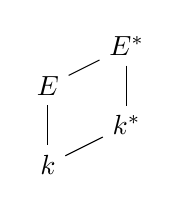
\begin{tikzpicture}
\node (1) at (0,0) {$E$};
\node (2) at (0,-1) {$k$};
\node (3) at (1,0.5) {$E^*$};
\node (4) at (1,-0.5) {$k^*$};
\draw (1) -- (2);
\draw (1) -- (3);
\draw (2) -- (4);
\draw (3) -- (4);
\end{tikzpicture}
\end{center}
Since \(k^*/k\) is normal, Theorem \ref{nthm3.17} gives
\(\Gal(E^*/k^*)\tril\Gal(E^*/k)\) and 
\begin{equation*}
\Gal(E^*/k)/\Gal(E^*/k^*)\cong\Gal(k^*/k)
\end{equation*}
Now\(\Gal(E^*/k^*)\) is solvable, while \(\Gal(k^*/k)\) is abelian, hence
solvable, by Proposition \ref{nprop3.12}. Finally, we may use Theorem
\ref{nthm3.17} once again, for the tower \(k\subseteq E\subseteq E^*\)
satisfies the hypothesis that both \(E\) and \(E^*\) are normal. It follows
that \(\Gal(E^*/k)/\Gal(E^*/E)\cong\Gal(E/k)\), and so \(G/k\), being a
quotient of a solvable group, is solvable
\end{proof}

\begin{theorem}[Abel-Ruffini]
If \(n\ge5\), the general polynomial
\begin{equation*}
f(x)=(x-y_1)(x-y_2)\cdots(x-y_n)
\end{equation*}
over a field \(k\) is not solvable by radicals
\end{theorem}
\begin{proof}
If \(E=k(y_1,\dots,y_n)\) and \(F=k(a_0,\dots,a_{n-1})\) where \(a_i\) are
the coefficients of \(f(x)\), then \(E\) is the splitting field of \(f(x)\)
over \(F\).

We claim that \(\Gal(E/F)\cong S_n\). Now if \(\sigma\in S_n\), then there
is an automorphism \(\widetilde{\sigma}\) of \(k[y_1,\dots,y_n]\), defined by 
\(\widetilde{\sigma}:f(y_1,\dots,y_n)\mapsto f(y_{\sigma 1},\dots,y_{\sigma n})\). Thus
\(\widetilde{\sigma}\) extends to an automorphism \(\sigma^*\) of 
\(E=\Frac(k[y_1,\dots,y_n])\) and \(\sigma^*\) fixes \(F\); hence
\(\sigma^*\in\Gal(E/F)\). Since \(\sigma\mapsto\sigma^*\) is an injection, 
\(\abs{S_n}\le\abs{\Gal(E/F)}\). 
On the other hand, Theorem \ref{nthm3.3} giving the reverse inequality.
Therefore \(\Gal(E/F)\cong S_n\). But \(S_n\) is not a solvable group if
\(n\ge5\), by Example \ref{nexample3.24}
\end{proof}




\section{Groups \rom{2}}
\label{sec:orgc22d514}
\subsection{Finite Abelian Groups}
\label{sec:orgda3cfdc}
\subsubsection{Direct Sums}
\label{sec:org1203c77}
\textbf{External direct sum}, denoted by \(S_1\times\cdots\times S_n\) is the
\(n\)-tuples \(s_1,\dots,s_n\), where \(s_i\in S_i\) for all \(i\), and its
binary operation is 
\begin{equation*}
(s_1,\dots,s_n)+(s_1',\dots,s_n')=(s_1+s_1',\dots,s_n+s_n')
\end{equation*}
However the most useful version, isomorphic to \(S_1\times\cdots\times S_n\)
is called their \textbf{internal direct sum}

\begin{definition}[]
If \(S\) and \(T\) are subgroups of an abelian group \(G\), then \(G\) is the
\textbf{direct sum}, denoted by
\begin{equation*}
G=S\oplus T
\end{equation*}
if \(S+T=G\) and \(S\cap T=\{0\}\)
\end{definition}

\begin{proposition}[]
The following statements are equivalent for an abelian group \(G\) and
subgroups \(S\) and \(T\) of \(G\)
\begin{enumerate}
\item \(G=S\oplus G\)
\item Every \(g\in G\) has a unique expression of the form
\begin{equation*}
g=s+t
\end{equation*}
where \(s\in S\) and \(t\in T\)
\item There are homomorphisms \(p:G\to S\) and \(q:G\to T\), called
\textbf{projections}, and \(i:S\to G\) and \(j:T\to G\) called \textbf{injections}, s.t.
\begin{equation*}
pi=1_S,\quad qj=1_T,\quad pj=0,\quad qi=0,\quad ip+jq=1_G
\end{equation*}
\end{enumerate}
\end{proposition}

\begin{corollary}[]
Let \(S\) and \(T\) be subgroups of an abelian group \(G\). If \(G=S\oplus T\),
then \(S\oplus T\cong S\times T\)

Conversely, given abelian group \(S\) and \(T\), define subgroups \(S'\cong S\)
and \(T'\cong T\) of \(S\times T\) by
\begin{equation*}
S'=\{(s,0):s\in S\}\quad\text{and}\quad T'=\{(0,t):t\in T\}
\end{equation*}
then \(S\times T=S'\oplus T'\)
\end{corollary}

\begin{definition}[]
If \(S_1,\dots,S_n,\dots\) are subgroups of an abelian group \(G\), define the
\textbf{finite direct sum} \(S_1\oplus\cdots\oplus S_n\) using induction on
\(n\ge2\):
\begin{equation*}
S_1\oplus\cdots\oplus S_{n+1}=[S_1\oplus\cdots\oplus S_n]\oplus S_{n+1}
\end{equation*}
We also denote the direct sum by
\begin{equation*}
\displaystyle\sum_{i=1}^nS_i=S_1\oplus\cdots\oplus S_n
\end{equation*}
\end{definition}

\begin{examplle}[]
Let \(V\) be a two-dimensional vector space over a field \(k\), which we view as
an additive abelian group, and let \(x,y\) be a basis. It's easy to check
that the intersection of any two of the subspaces \(\la x\ra\), 
\(\la y\ra\) and \(\la x+y\ra\) is \(\{0\}\). On the other hand, we do not
have
\(V=[\la x\ra\oplus\la y\ra]\oplus\la x+y\ra\) because
\([\la x\ra\oplus\la y\ra]\cap\la x+y\ra\neq\{0\}\)
\end{examplle}

In the context of abelian groups, we shall write \(S\subseteq G\) to denote
\(S\) being a subgroup of \(G\).


\begin{proposition}[]
\label{prop5.4}
Let \(G=S_1+\cdots+S_n\), where the \(S_i\) are subgroups. Then the following
conditions are equivalent
\begin{enumerate}
\item \(G=S_1\oplus\cdots\oplus S_n\)
\item Every \(a\in G\) has a unique expression of the form
\(a=s_1+\cdots+s_n\), where \(s_i\in S_i\)
\item For each \(i\)
\begin{equation*}
S_i\cap(S_1+\cdots+\widehat{S_i}+\cdots+S_n)=\{0\}
\end{equation*}
where \(\widehat{S_i}\) means that the term \(S_i\) is omitted from the
sum
\end{enumerate}
\end{proposition}

\begin{corollary}[]
Let \(G=\la y_1,\dots,y_n\ra\). If for all \(m_i\in\Z\), we have
\(\sum_im_iy_i=0\) implies \(m_iy_i=0\); then
\begin{equation*}
G=\la y_1\ra\oplus\cdots\oplus\la y_n\ra
\end{equation*}
\end{corollary}

\begin{examplle}[]
Let \(V\) be an \(n\)-dimensional vector space over a filed \(k\), which we view
as an additive abelian group. If \(v_1,\dots,v_n\) is a basis, then
\begin{equation*}
V=\la v_1\ra\oplus\cdots\oplus\la v_n\ra
\end{equation*}
where \(\la v_i\ra=\{rv_i:r\in k\}\)
\end{examplle}

\begin{proposition}[]
\label{prop5.7}
If \(G_1,\dots,G_n\) are abelian groups and \(H_i\subseteq G_i\) are
subgroups, then
\begin{equation*}
(G_1\oplus\cdots\oplus G_n)/(H_1\oplus\cdots\oplus H_n)\cong(G_1/H_1)
\times\cdots\times(G_n/H_n)
\end{equation*}
\end{proposition}

If \(G\) is an abelian group and \(m\) is an integer, let us write
\begin{equation*}
mG=\{ma:a\in G\}
\end{equation*}

\begin{proposition}[]
If \(G\) is an abelian group and \(p\) is a prime, then \(G/pG\) is a vector
space over \(\F_p\)
\end{proposition}

\begin{proof}
If \([r]\in\F_p\) and \(a\in G\), define scalar multiplication
\begin{equation*}
[r](a+pG)=ra+pG
\end{equation*}
\end{proof}

\begin{definition}[]
Let \(F=\la x_1,\dots,x_n\ra\) be an abelian group. If 
\begin{equation*}
F=\la x_1\ra\oplus\cdots\oplus\la x_n\ra
\end{equation*}
where each \(\la x_z\ra\cong\Z\), then \(F\) is called a (finitely generated) 
\textbf{free abelian group} with \textbf{basis} \(x_1,\dots,x_n\)
\end{definition}

\begin{proposition}[]
If \(\Z^m\) denotes the direct sum of \(m\) copies of \(\Z\), then
\(\Z^m\cong\Z^n\) if and only if \(m=n\)
\end{proposition}

\begin{proof}
For any abelian group \(G\), if \(G=G_1\oplus\cdots\oplus G_n\), then
\(2G=2G_1\oplus\cdots\oplus 2G_n\). It follows from Proposition \ref{prop5.7}
that
\begin{equation*}
G/2G\cong(G_1/2G_1)\oplus\cdots\oplus(G_n/2G_n)
\end{equation*}
so that \(\abs{G/2G}=2^n\). Since \(G/2G\cong H/2H\)
\end{proof}

\begin{corollary}[]
If \(F\) is a (finitely generated) free abelian group, then any two bases of
\(F\) have the same number of elements
\end{corollary}

\begin{proof}
If \(x_1,\dots,x_n\) is a basis of \(F\), then \(F\cong\Z^n\)
\end{proof}

\begin{definition}[]
If \(F\) is a free abelian group with basis \(x_1,\dots,x_n\), then \(n\) is
called the \textbf{rank} of \(F\), and we write \(\rank(F)=n\)
\end{definition}

The rank of free abelian group plays the same role as the dimension of a
vector space.

\begin{theorem}[]
\label{thm5.11}
Let \(F\) be a free abelian group with basis \(X=\{x_1,\dots,x_n\}\). If \(G\)
is any abelian group and if \(\gamma:X\to G\) is any function, then there exists
a unique homomorphism \(g:F\to G\) with \(g(x_i)=\gamma(x_i)\)

\begin{center}
\begin{tikzcd}
F\arrow[dr,dashed,"g"]\\
X\arrow[u]\arrow[r,"\gamma"']&G
\end{tikzcd}
\end{center}
\end{theorem}

\begin{proposition}[]
Let \(A\) be an abelian group containing a subset \(X=\{x_1,\dots,x_n\}\), and
let \(A\) have the property in \ref{thm5.11}. Then \(A\cong\Z^n\)
\end{proposition}

\begin{proof}
Consider
\begin{center}
\begin{tikzcd}
A\arrow[dr,dashed,"g"]\\
X\arrow[u,"p"]\arrow[r,"q"']&\Z^n
\end{tikzcd}
\hspace{0.2cm}
and
\hspace{0.4cm}
\begin{tikzcd}
\Z^n\arrow[dr,dashed,"h"]\\
X\arrow[u,"q"]\arrow[r,"\gamma"']&A
\end{tikzcd}
\end{center}
\end{proof}
\subsubsection{Basis Theorem}
\label{sec:orged23663}
\begin{definition}[]
If \(p\) is a prime, then an abelian group \(G\) is \textbf{\(p\)-primary} if for each
\(a\in G\), there is \(n\ge 1\) with \(p^na=0\)

If \(G\) is any abelian group, then its \textbf{\(p\)-primary component} is 
\begin{equation*}
G_p=\{a\in G:p^na=0\text{ for some }n\ge1\}
\end{equation*}
\end{definition}


\begin{theorem}[Primary Decomposition]
\begin{enumerate}
\item Every finite abelian group \(G\) is a direct sum of its \(p\)-primary
components
\begin{equation*}
G=G_{p_1}\oplus\cdots\oplus G_{p_n}
\end{equation*}
\item Two finite abelian groups \(G\) and \(G'\) are isomorphic if and only if
\(G_p\cong G_p'\) for every prime \(P\)
\end{enumerate}
\end{theorem}

\begin{proof}
Let \(x\in G\) be nonzero, and let its order be \(d\).
\begin{equation*}
d=p_1^{e_1}\dots p_n^{e_n}
\end{equation*}
Define \(r_i=d/p_i^{e_i}\). It follows that \(r_ix\in G_{p_i}\). But the gcd
of \(r_1,\dots,r_n\) is 1, hence \(1=\sum_is_ir_i\). Therefore
\begin{equation*}
x=\displaystyle\sum_{i}s_ir_ix\in G_{p_1}+\cdots+G_{p_n}
\end{equation*}
Write \(H_i=G_{p_1}+\cdots+\widehat{G_{p_i}}+\cdots+G_{p_n}\). By
Proposition \ref{prop5.4}, it suffices to prove that 
\(G_{p_i}\cap H_i=\{0\}\). If \(x\in G_{p_i}\cap H_i\), \(p_i^lx=0\), 
\(x=\sum_{j\neq i}y_j\) where \(p_j^{g_j}y_j=0\). Hence 
\(ux=0\) where \(u=\prod_{j\neq i}p_j^{g_j}\). But \(p_i^l\) and \(u\) are
relatively prime, so \(1=sp_i^l+tu\). Therefore
\begin{equation*}
x=(sp_i^l+tu)x=0
\end{equation*}
\end{proof}

\begin{definition}[]
Let \(p\) be a prime and let \(G\) be a \(p\)-primary abelian group. A subgroup
\(S\subseteq G\) is a \textbf{pure subgroup} if for all \(n\ge 0\)
\begin{equation*}
S\cap p^nG=p^nS
\end{equation*}
\end{definition}

If \(s=p^ng\), then there is a \(s'\in S\) s.t. \(s=p^ns'\)

\begin{lemma}[]
If \(p\) is a prime and \(G\) is a finite 
\#+BEGIN\textsubscript{lemma}
\end{lemma}
\section{Commutative Rings \rom{2}}
\label{sec:org5875fa5}
\subsection{Prime Ideals and Maximal Ideals}
\label{sec:org89aac70}
\begin{proposition}[Correspondence Theorem for Rings]
If \(I\) is a proper ideal in a commutative ring \(R\), then there is an
inclusion-preserving bijection \(\varphi\) from the set of all intermediate ideals \(J\)
containing \(I\), that is, \(I\subseteq J\subseteq R\), to the set of all the
ideals in \(R/I\), given by
\begin{equation*}
\varphi:J\mapsto\pi(J)=J/I
\end{equation*}
where \(\pi\) is the natural map
\begin{center}
\begin{tikzcd}
R \arrow[d,dash] \arrow[rd]&\\
J' \arrow[d,dash] \arrow[rd] & R/I \arrow[d,dash]\\
J \arrow[d,dash] \arrow[rd] & J'/I \arrow[d,dash]\\
I  \arrow[rd] & J/I \arrow[d,dash]\\
& \{0\}
\end{tikzcd}
\end{center}
\end{proposition}

\begin{proof}
If we forget its multiplication, the commutative ring \(R\) is merely an
additive group and its ideal is a (normal) subgroup. Theorem \ref{thm2.76}
gives an inclusion-preserving bijection
\begin{equation*}
\Phi:\{\text{all subgroups of $R$ containing $I$}\}\to 
\{\text{all subgroups of $R/I$}\}
\end{equation*}
where \(\Phi(J)=\pi(J)=J/I\)

If \(J\) is an ideal, then \(\Phi(J)\) is also an ideal.
\end{proof}

In practice, the correspondence theorem is invoked, tacitly, by saying that
every ideal in the quotient ring \(R/I\) has the form \(J/I\) for some ideal
\(J\) with \(I\subseteq J\subseteq R\)

\begin{examplle}[]
Let \(I=(m)\) be a nonzero ideal in \(\Z\). If \(J\) is an ideal in \(\Z\)
containing \(I\), then \(J=(a)\) for some \(a\in\Z\) because \(\Z\) is a PID
and \((m)\subseteq(a)\) iff \(a\mid m\). The correspondence theorem shows
that every ideal in \(\I_m\) has the form \(([a])\) for some divisor \(a\) of \(m\)
\end{examplle}

\begin{definition}[]
An ideal \(I\) in a commutative ring \(R\) is called a \textbf{prime ideal} if it is a
proper ideal and \(ab\in I\) implies \(a\in I\) or \(b\in I\)
\end{definition}

\begin{examplle}[]
We claim that the prime ideals in \(\Z\) are precisely the ideals \((p)\),
where either \(p\) is 0 or a prime.
\end{examplle}

\begin{proposition}[]
An ideal \(I\) in a commutative ring \(R\) is a prime ideal if and only if
\(R/I\) is a domain
\end{proposition}

\begin{proposition}[]
If \(K\) is a field, then a nonzero polynomial \(p(x)\in k[x]\) is irreducible
if and only if \((p(x))\) is a prime ideal
\end{proposition}

\begin{proof}
Suppose that \(p(x)\) is irreducible. First \((p(x))\) is a proper ideal.
Otherwise \(1\in (p(x))\), so there is a polynomial \(f(x)\) with
\(1=p(x)f(x)\). But \(p(x)\) has degree at least 1

Second, if \(ab\in(p)\), then \(p\mid ab\), and Euclid's lemma in \(k[x]\)
gives \(p\mid a\) or \(p\mid b\)
\end{proof}

\begin{definition}[]
An ideal \(I\) in a commutative ring \(R\) is a \textbf{maximal ideal} if it is a proper
ideal and there is no ideal \(J\) with \(I\not\subseteq J\not\subseteq R\)
\end{definition}

\begin{proposition}[]
A proper ideal \(I\) in a nonzero commutative ring \(R\) is a maximal ideal if
and only if \(R/I\) is a field
\end{proposition}

\begin{proof}
The correspondence theorem shows that \(I\) is maximal if and only if \(R/I\)
has no ideals other than \(\{0\}\) and \(R/I\)
\end{proof}

\begin{corollary}[]
\label{cor6.8}
Every maximal ideal \(I\) in a commutative ring \(R\) is a prime ideal
\end{corollary}

\begin{examplle}[]
The converse of Corollary \ref{cor6.8} is false. Consider the principal ideal
\((x)\) in \(\Z[x]\). By Exercise \ref{ex3.83}
\begin{equation*}
\Z[x]/(x)\cong\Z
\end{equation*}
since \(\Z\) is a domain, \(x\) is a prime ideal. Since \(\Z\) is not a field,
\((x)\) is not a maximal ideal. Let 
\begin{equation*}
J=\{f(x)\in\Z[x]:f(x)\text{ has even constant term}\}
\end{equation*}
Since \(\Z[x]/J\cong\F_2\) is a field, it follows that \(J\) is a maximal ideal
containing \((x)\)
\end{examplle}

\begin{examplle}[]
Let \(k\) be a field, and let \(a=(a_1,\dots,a_n)\in k^n\). Define the
\textbf{evaluation map}
\begin{equation*}
e_a:k[x_1,\dots,x_n]\to k
\end{equation*}
by
\begin{equation*}
e_a:f(x_1,\dots,x_n)\mapsto f(a)
\end{equation*}
\(e_a\) is a surjective ring homomorphism, and so \(\ker e_a\) is a maximal
ideal
\end{examplle}

\begin{theorem}[]
If \(R\) is a PID, then every nonzero prime ideal \(I\) is a maximal ideal
\end{theorem}

\begin{proof}
Assume that there is a proper ideal \(J\) with \(I\subseteq J\). Since \(R\) is a
PID, \(I=(a)\) and \(I=(b)\) for some \(a,b\in R\). Now \(a\in J\) implies
that \(a=rb\) for some \(r\in R\) and so \(rb\in I\). Since \(I\) is prime,
either \(r\in I\) or \(b\in I\). If \(r\in I\), then \(r=ta\) for some 
\(t\in I\), and \(a=tab=atb\). Since \(R\) is a domain, \(1=tb\). Hence \(J=R\)
\end{proof}

\begin{corollary}[]
If \(k\) is a field and \(p(x)\in k[x]\) is irreducible, then the quotient ring 
\(k[x]/(p(x))\) is a field
\end{corollary}

\begin{proof}
Since \(p(x)\) is irreducible, \((p(x))\) is a prime ideal. Since \(k[x]\) is
a PID, \((p(x))\) is maximal
\end{proof}

\begin{proposition}[]
Let \(P\) be a prime ideal in a commutative ring \(R\). If \(I\) and \(J\) are ideals
with \(IJ\subseteq P\), then \(I\subseteq P\) or \(J\subseteq P\)
\end{proposition}

\begin{proof}
Suppose, on the contrary, that \(I\not\subseteq P\) and \(J\not\subseteq P\);
thus there are \(a\in I\) and \(b\in J\) with \(a,b\not\in P\). But 
\(ab\in IJ\subseteq P\), contradicting \(P\) being prime
\end{proof}

\begin{proposition}[]
Let \(B\) be a subset of a commutative ring \(R\) which is closed under addition
and multiplication
\begin{enumerate}
\item Let \(J_1,\dots,J_n\) be ideals in \(R\), at least \(n-2\) which are prime.
If \(B\subseteq J_1\cup\cdots\cup J_n\), then \(B\) is contained in some
\(J_i\)
\item Let \(I\) be an ideal in \(R\) with \(I\subsetneq B\). If there are prime
ideals \(P_1,\dots,P_n\) s.t. \(B-I\subseteq P_1\cup\dots\cup P_n\), then 
\(B\subseteq P_i\) for some \(i\)
\end{enumerate}
\end{proposition}

\begin{proof}
\begin{enumerate}
\item Induction on \(n\ge2\). If \(B\not\subseteq J_2\), then there is \(b_1\in B\)
with \(b_1\not\in J_2\), and hence \(b_1\in J_1\). If \(B\not\subseteq J_1\),
there is \(b_2\in B\) with \(b_2\not\in J_1\) and \(b_2\in J_2\). However if
\(y=b_1+b_2\), then \(y\not\in J_1\) and \(y\not\in J_2\), contradicting 
\(B\subseteq J_1\cup J_2\)

For the inductive step, assume that \(B\subseteq J_1\cup\cdots\cup J_{n+1}\),
where at least \(n-1=(n+1)-2\) of the \(J_i\) are prime ideals. Let
\begin{equation*}
D_i=J_1\cup\cdots\cup\widehat{J_i}\cup\cdots\cup J_{n+1}
\end{equation*}
the inductive hypothesis allows us to assume that \(B\not\subseteq D_i\) for
all \(i\). Hence for all \(i\), there exists \(b_i\in B\) with 
\(b_i\not\in D_i\); since \(B\subseteq D_i\cup J_i\), we must have 
\(b_i\in J_i\). Now \(n\ge3\), so that at least one of the \(J_i\) is a prime
ideal. Assume \(J_1\) is prime. Consider the elements
\begin{equation*}
y=b_1+b_2b_3\dots b_{n+1}
\end{equation*}
\(y\not\in J_i\) for any i
\item \(B\subseteq I\cup P_1\cup\cdots\cup P_n\)
\end{enumerate}
\end{proof}
\subsection{Unique Factorization Domains}
\label{sec:org65f4b01}
\index{associate}
\begin{definition}[]
Elements \(a\) and \(b\) in a commutative ring \(R\) are \textbf{associates} if there exists
a unit \(u\in R\) with \(b=ua\)
\end{definition}

\begin{proposition}[]
Let \(R\) be a domain and let \(a,b\in R\)
\begin{enumerate}
\item \(a\mid b\) and \(b\mid a\) if and only if \(a\) and \(b\) are associates
\item The principal ideals \((a)\)  and \((b)\) are equal if and only if \(a\)
and \(b\) are associates
\end{enumerate}
\end{proposition}

\begin{corollary}[]
If \(R\) is a PID and \(p\in R\) is irreducible, then \((p)\) is a prime ideal
\end{corollary}

\begin{proof}
\((p)\) is maximal
\end{proof}

\index{ UFD}
\begin{definition}[]
A domain \(R\) is a \textbf{unique factorization domain} (\textbf{UFD}) if
\begin{enumerate}
\item every \(r\in R\), neither 0 nor a unit, is a product of irreducibles
\item if \(up_1\dots p_m=vq_1\dots q_n\), where \(u\) and \(v\) are units and
\(p_i,q_i\) are irreducible, then \(m=n\) and there is a permutation
\end{enumerate}
\(\sigma\in S_n\) with \(p_i\) and \(q_{\sigma(i)}\) associates for all \(i\)
\end{definition}

\begin{proposition}[]
\label{prop6.17}
Let \(R\) be a domain in which every \(r\in R\), neither 0 nor a unit, is a
product of irreducibles. Then \(R\) is a UFD if and only if \((p)\) is a prime
ideal in \(R\) for every irreducible element \(p\in R\)
\end{proposition}

\begin{proof}
Assume that \(R\) is a UFD. If \(a,b\in R\) and \(ab\in(p)\), then there is
\(r\in R\) with
\begin{equation*}
ab=rp
\end{equation*}
Factor each of \(a,b,r\) into irreducibles; by unique factorization, the left
side of the equation must involve an associate of \(p\)

Assume that 
\begin{equation*}
up_1\dots p_m=vq_1\dots q_n
\end{equation*}
where \(p_i\) and \(q_j\) are irreducibles and \(u,v\) are units. We prove,
by induction on \(\max\{m,n\}\ge1\). If \(\max{m,n}=1\), then 
\(up_1=v,u=vq_1\) or \(up_1=vq_1\). The first two cannot happen, and so the
base step is true. For the inductive steop, the given equation shows that 
\(p_1\mid q_1\dots q_n\). By hypothesis, \((p_1)\) is a prime ideal, and so
there is some \(q_j\) with \(p_1\mid q_j\), so that \(p_1\) and \(q_j\) are
associates. Canceling \(p_1\) from both side.
\end{proof}

\begin{lemma}[]
\begin{enumerate}
\item If \(R\) is a commutative ring and
\begin{equation*}
I_1\subseteq I_2\subseteq\cdots\subseteq I_n\subseteq\cdots
\end{equation*}
is an ascending chain of ideals of \(R\), then \(J=\bigcup_{n\ge1}I_n\) is
an ideal in \(R\)
\item If \(R\) is a PID, then it has no infinite strictly ascending chain of
ideals 
\begin{equation*}
I_1\subsetneq I_2\subsetneq\cdots\subsetneq I_n\subsetneq\cdots
\end{equation*}
\item Let \(R\) be a PID. If \(r\in R\) is neither 0 nor a unit, then \(r\) is a
product of irreducibles
\end{enumerate}
\end{lemma}

\begin{proof}
\begin{enumerate}
\item If \(a\in J\), then \(a\in I_n\) for some \(n\); if \(r\in R\), then 
\(ra\in I_n\); hence \(ra\in J\). If \(a,b\in J\), then \(a\in I_m\) and 
\(a\in I_n\)\ldots{}
\item \(J\) is principal ideal domain and \(J=(d)\), then
\begin{equation*}
J=(d)\subseteq I_n\subsetneq I_{n+1}\subseteq J
\end{equation*}
\item A divisor \(r\) of an element \(a\in R\) is called a \textbf{proper divisor} of \(a\).
Call a nonzero nonunit \(a\in R\) \textbf{good} if it is a product of irreducibles.
If \(a\) is bad, then \(a=rs\), where both \(r\) and \(s\) are proper
divisors. But the product of good elements is good, and so at least one of
the factors, say \(r\), is bad. It follows , by induction, that there exists
a sequence \(a_1=a,a_2=r,a_3,\dots,a_n,\dots\) of bad elements and yields
a strictly ascending chain
\begin{equation*}
(a_1)\subsetneq(a_2)\subsetneq\dots
\end{equation*}
\end{enumerate}
\end{proof}

\begin{theorem}[]
If \(R\) is a PID, then \(R\) is a UFD.
\end{theorem}

\begin{proposition}[]
If \(R\) is a UFD, then a gcd of any finite set of elements \(a_1,\dots, a_n\)
in \(R\) exists
\end{proposition}

\begin{proof}
\begin{align*}
&a=up_1^{e_1}\dots p_t^{e_t}\\
&b=vp_1^{f_1}\dots p_t^{f_t}
\end{align*}
where \(e_i,f_i\ge0\)
\end{proof}

\begin{definition}[]
Elements \(a_1,\dots,a_n\) in a UFD \(R\) is called \textbf{relatively prime} if their
gcd is a unit
\end{definition}

\index{primitive polynomial}
\begin{definition}[]
A polynomial \(f(x)=a_nx^n+\dots+a_1x+a_0\in R[x]\), where \(R\) is a UFD, is
called \textbf{primitive} if its coefficients are relatively prime
\end{definition}

\begin{examplle}[]
For a UFD \(R\), every irreducible \(p(x)\in R[x]\) of positive degree is
primitive. 
\end{examplle}

\begin{lemma}[Gauss's Lemma]
If \(R\) is a UFD and \(f(x),g(x)\in R[x]\) are both primitive, then their
product \(f(x)g(x)\) is also primitive
\end{lemma}

\begin{proof}
If \(\pi:R\to R/(p)\) is the natural map \(\pi:a\mapsto a+(p)\), then Proposition
\ref{prop3.48} shows that the function \(\widetilde{\pi}:R[x]\to(R/(p))[x]\) is a
ring homomorphism. If a polynomial \(h(x)\in R[x]\) is not primitive, there is
some irreducible \(p\) s.t. all the coefficients of \(\widetilde{\pi}(h)\) are 0
in \(R/(p)\); that is, \(\widetilde{\pi}(h)=0\) in \(R/(p)[x]\). Thus, if the
product \(f(x)g(x)\) is not primitive, there is some irreducible \(p\) with 
\(0=\widetilde{\pi}(fg)=\widetilde{\pi}(f)\widetilde{\pi}(g)\). Since \((p)\) is a
prime ideal, \(R/(p)\) is a domain, and hence \((R/(p))[x]\) is also a
domain. But neither \(\widetilde{\pi}(f)\) nor \(\widetilde{\pi}(g)\) are 0 in
\((R/(p))[x]\), a contradiction
\end{proof}

\begin{lemma}[]
\label{lemma6.24}
Let \(R\) be a UFD, let \(Q=\Frac(R)\), and let \(f(x)\in Q[x]\) be nonzero
\begin{enumerate}
\item There is a factorization
\begin{equation*}
f(x)=c(f)f^*(x)
\end{equation*}
where \(c(f)\in Q\) and \(f^*(x)\in R[x]\) is primitive. This
factorization is unique in the sense that if \(f(x)=qg^*(x)\), where
\(q\in Q\) and \(g^*(x)\in R[x]\) is primitive, then there is a unit 
\(w\in R\) with \(q=wc(f)\) and \(g^*(x)=w^{-1}f^*(x)\)
\item If \(f(x),g(x)\in R[x]\), then \(c(fg)\) and \(c(f)c(g)\) are associates
in \(R\) and \((fg)^*\) and \(f^*g^*\) are associates in \(R[x]\)
\item Let \(f(x)\in Q[x]\) have a factorization \(f(x)=qg^*(x)\), where 
\(q\in Q\) and \(g^*(x)\in R[x]\) is primitive. Then \(f(x)\in R[x]\) if
and only if \(q\in R\)
\item Let \(g^*(x),f(x)\in R[x]\). If \(g^*(x)\) is primitive and 
\(g^*(x)\mid b f(x)\), where \(b\in R\) and \(b\neq0\), then 
\(g^*(x)\mid f(x)\)
\end{enumerate}
\end{lemma}

\begin{proof}
\begin{enumerate}
\item Clearing denominators, there is \(b\in R\) with \(bf(x)\in R[x]\). If
\(d\) is the gcd of the coefficients of \(bf(x)\), then \((b/d)f(x)\in
      R[x]\) is a primitive polynomial. If we define \(c(f)=d/b\) and 
\(f^*(x)=(b/d)f(x)\)

Suppose \(c(f)f^*(x)=qg^*(x)\). Exercise \ref{ex6.17} allows use to write
\(q/c(f)\) in lowest terms: \(q/c(f)=u/v\). The equation 
\(vf^*(x)=ug^*(x)\) holds in \(R[x]\). Since \(v,u\) are relatively prime
and \(g^*(x)\) is primitive, \(v\) is a unit

\setcounter{enumi}{3}
\item Since \(bf=hg^*\), we have \(bc(f)f^*=c(h)h^*g^*=c(h)(hg)^*\). By
uniqueness, \(f^*\) and \((hg)^*\) are associates
\end{enumerate}
\end{proof}

\begin{definition}[]
Let \(R\) be a UFD with \(Q=\Frac(R)\). If \(f(x)\in Q[x]\), there is a
factorization \(f(x)=c(f)f^*(x)\), where \(c(f)\in Q\) and 
\(f^*(x)\in R[x]\) is primitive. We call \(c(f)\) the \textbf{content} of \(f(x)\) and
\(f^*(x)\) the \textbf{associated primitive polynomial}
\end{definition}

\begin{theorem}[Gauss]
If \(R\) is a UFD, then \(R[x]\) is also a UFD
\end{theorem}

\begin{proof}
We show first, by induction on \(\deg(f)\), that every \(f(x)\in R[x]\),
neither 0 nor a unit, is a product of irreducibles. If \(\deg(f)>0\), then 
\(f(x)=c(f)f^*(x)\) where \(c(f)\in R\) and \(f^*(x)\) is primitive. If
\(f^*(x)\) is irreducible, we are done. Otherwise \(f^*(x)=g(x)h(x)\), where
neither \(g\) nor \(h\) is a unit. And so each is is a product of irreducibles,
by the inductive hypothesis

Now Proposition \ref{prop6.17} applies: \(R[x]\) is a UFD if \((p(x))\) is a
prime ideal for every irreducible \(p(x)\in R[x]\). Let's assume 
\(p\mid fg\) and \(p\nmid f\)

Case (i). Suppose that \(\deg(p)=0\) . Write
\begin{equation*}
f(x)=c(f)f^*(x),\quad g(x)=c(g)g^*(x)
\end{equation*}
Now \(p\mid fg\), so that
\begin{equation*}
p\mid c(f)c(g)f^*(x)g^*(x)
\end{equation*}
Since \(f^*(x)g^*(x)\) is primitive, Lemma \ref{lemma6.24} says that
\(c(f)c(g)\) is an associate of \(c(fg)\). However, if \(p\mid fg\), then \(p\)
divides each coefficient of \(fg\); that is, \(p\) is a common divisor of all
coefficients of \(fg\), and hence in \(R\), which is a UFD, \(p\) divides the
associates \(c(fg)\) and \(c(f)c(g)\). But Proposition \ref{prop6.17} says that
\((p)\) is a prime ideal, and so \(p\mid c(f)\) or \(p\mid c(g)\). Therefore
\(p\mid c(g)\)

Case (ii). Suppose that \(\deg(p)>0\). Let 
\begin{equation*}
(p,f)=\{s(x)p(x)+t(x)f(x):s(x),t(x)\in R[x]\}
\end{equation*}
Choose \(m(x)\in(p,f)\) of minimal degree. If \(Q=\Frac(R)\) is the fraction
field of \(R\), then the division algorithm in \(Q[x]\) gives polynomials
\(q'(x),r'(x)\in Q[x]\) with
\begin{equation*}
f(x)=m(x)q'(x)+r'(x)
\end{equation*}
where either \(r'(x)=0\) or \(\deg(r')<\deg(m)\). Clearing denominators,
there are polynomials \(q(x),r(x)\in R[x]\) and a constant \(b\in R\) with
\begin{equation*}
bf(x)=q(x)m(x)+r(x)
\end{equation*}
Since \(m\in(p,f)\), there are polynomials \(s(x),t(x)\in R[x]\) with 
\(m=sp+tx\); hence \(r=bf-qm\in(b,f)\). Since \(m\) has minimal degree, we
must have \(r=0\); that is, \(bf(x)=q(x)m(x)\), and so
\(bf(x)=c(m)m*(x)q(x)\). So that \(m^*(x)\mid f(x)\) by Lemma \ref{lemma6.24}.
A similar argument, replacing \(f(x)\) by \(p(x)\), gives 
\(m^*(x)\mid p(x)\). If \(m^*(x)\) were an associate of \(p(x)\), then
\(p(x)\mid f(x)\), contrary to hypothesis. Hence \(m^*(x)\) is a unit; that
is, \(m(x)=c(m)\in R\), and so \(p,f\) contains the nonzero constant
\(c(m)\). Now \(c(m)=sp+tf\), and so
\begin{equation*}
c(m)g(x)=s(x)p(x)g(x)+t(x)f(x)g(x)
\end{equation*}
Since \(p\mid fg\), we have \(p(x)\mid c(m)g(x)\). But \(p(x)\) is primitive, 
\(p(x)\mid g(x)\)
\end{proof}

\begin{corollary}[]
If \(k\) is a field, then \(k[x_1,\dots,x_n]\) is a UFD
\end{corollary}

\begin{corollary}[Gauss]
\label{ncor5.28}
Let \(R\) be a UFD, let \(Q=\Frac(R)\), and let \(f(x)\in R[x]\) . If 
\begin{equation*}
f(x)=G(x)H(x)\in Q[x]
\end{equation*}
then there is a factorization
\begin{equation*}
f(x)=g(x)h(x)\in R[x]
\end{equation*}
where \(\deg(g)=\deg(G)\) and \(\deg(h)=\deg(H)\); in fact, \(G(x)\) is a
constant multiple of \(g(x)\) and \(H(x)\) is a constant multiple of
\(h(x)\). Therefore, if \(f(x)\) does not factor into polynomials of smaller
degree in \(R[x]\), then \(f(x)\) is irreducible in \(Q[x]\)
\end{corollary}

\begin{examplle}[]
We claim that \(f(x,y)=x^2+y^2-1\in k[x,y]\) is irreducible, where \(k\) is a
field. Write \(Q=k(y)=\Frac(k[y])\), and view \(f(x,y)\in Q[x]\). Now the
quadratic \(g(x)=x^2+(y^2-1)\) is irreducible in \(Q[x]\) iff it has no roots
in \(Q=k(y)\), and this is so by Exercise \ref{ex3.34}

It follows from Proposition \ref{prop6.17} that \((x^2+y^2-1)\) is a prime
ideal because it is generated by an irreducible polynomial
\end{examplle}

\begin{proposition}[]
\label{nprop5.30}
Let \(k\) be a field, and view \(f(x_1,\dots,x_n)\in k[x_1,\dots,x_n]\) as a
polynomial in \(R[x_n]\), where \(R=k[x_1,\dots,x_{n-1}]\)
\begin{equation*}
f(x_n)=a_0(x_1,\dots,x_{n-1})+\dots+a_m(x_1,\dots,x_{n-1})x^m_n
\end{equation*}
If \(f(x_n)\) is primitive and cannot be factored into two polynomials of
lower degree in \(R[x_n]\), then \(f(x_1,\dots,x_n)\) is irreducible in
\(k[x_1,\dots,x_n]\) 
\end{proposition}

\begin{proof}
Suppose that \(f(x_n)=g(x_n)h(x_n)\) in \(R[x_n]\); by hypothesis, the
degrees of \(g\) and \(h\) in \(x_n\) cannot both be less than \(\deg(f)\); say,
\(\deg(g)=0\). It follows, because \(f\) is primitive, that \(g\) is a unit in
\(k[x_1,\dots,x_{n-1}]\). Therefore, \(f(x_1,\dots,x_n)\) is irreducible in \(R[x_n]\)
\end{proof}

\begin{corollary}[]
\label{ncor5.31}
If \(k\) is a field and 
\(g(x_1,\dots,x_n),h(x_1,\dots,x_n)\in k[x_1,\dots,x_n]\) are relatively
prime, then \(f(x_1,\dots,x_n,y)=yg(x_1,\dots,x_n)+h(x_1,\dots,x_n)\) is
irreducible in \(k[x_1,\dots,x_n,y]\)
\end{corollary}

\begin{proof}
Let \(R=k[x_1,\dots,x_n]\). Note that \(f\) is primitive in \(R[y]\), because
\((g,h)=1\) forces any divisor of its coefficients \(g,h\) to be a unit.
Since \(f\) is linear in \(y\), it is not the product of two polynomials in \(R[y]\)
of smaller degree, and hence Proposition \ref{nprop5.30} shows that \(f\) is
irreducible in \(R[y]=k[x_1,\dots,x_n,y]\)
\end{proof}

\begin{examplle}[]
The polynomials \(x\) and \(y^2+z^2-1\) are relatively prime in \(\R[x,y,z]\),
so that \(f(x,y,z)=x^2+y^2+z^2-1\) is irreducible
\end{examplle}


\begin{corollary}[]
If \(\alpha\) is an algebraic integer, then \(\irr(\alpha,\Q)\) lies in \(\Z[x]\)
\end{corollary}


\begin{definition}[]
If \(\alpha\) is an algebraic integer, then its \textbf{minimal polynomial} is the monic
polynomial in \(\Z[x]\) of least degree having \(\alpha\) as a root.
\end{definition}

\begin{remark}
We define the (algebraic) \textbf{conjugates} of \(\alpha\) to be the roots of \(\irr(\alpha,\Q)\),
and we define the \textbf{norm} of \(\alpha\) to be the absolute value of the product of the
conjugates \(\alpha\)
\end{remark}

\begin{theorem}[]
Let \(f(x)=a_0+a_1x+\dots+x^n\in\Z[x]\) be monic, and let \(p\) be a prime. If
\(f(x)\) is irreducible\(\mod p\), that is, if
\begin{equation*}
\widetilde{f}(x)=[a_0]+[a_1]x+\dots+x^n\in\F_p[x]
\end{equation*}
is irreducible, then \(f(x)\) is irreducible in \(\Q[x]\)
\end{theorem}

\begin{proof}
By Proposition \ref{prop3.48}, the natural map \(\varphi:\Z\to\F_p\) defines a
homomorphism \(\widetilde{\varphi}:\Z[x]\to\F_p\). If \(g(x)\in\Z[x]\), define its
image \(\widetilde{\varphi}(g(x))\in\F_p[x]\) by \(\widetilde{g}(x)\). Prove
\(f(x)\) is irreducible in \(\Z[x]\). Then by Gauss's theorem, \(f(x)\) is
irreducible in \(\Q[x]\)
\end{proof}



\begin{exercise}
\label{ex6.17}
Let \(R\) be a UFD and let \(Q=\Frac{R}\) be its fraction field. Prove that
each nonzero \(a/b\in Q\) has an expression in lowest terms; that is, \(a\)
and \(b\) are relatively prime.
\end{exercise}

\begin{proof}
there gcd exists
\end{proof}

\begin{exercise}
\label{ex6.18}
Let \(R\) be a UFD
\begin{enumerate}
\item If \(a,b,c\in R\) and \(a\) and \(b\) are relatively prime, prove that 
\(a\mid bc\) implies \(a\mid c\)
\item If \(a,c_1,\dots,c_n\in R\) and \(c_i\mid a\) for all \(i\), prove that 
\(c\mid a\), where \(c=\lcm\{c_1,\dots,c_n\}\)
\end{enumerate}
\end{exercise}

\begin{examplle}[]
\begin{enumerate}
\item We show that \(f(x)=x^4-5x^3+2x+3\)  is an irreducible polynomial in
\(\Q[x]\)

The only candidates for rational roots are \(1,-1,3,-3\) and none of these
is a root.

Since \(\widetilde{f}(x)=x^4+x^3+1\in\F_2[x]\) is irreducible by Example
\ref{example3.35}, it follows that \(f(x)\) is irreducible in \(\Q[x]\).

\item Let \(\Phi_5(x)=x^4+x^3+x^2+x+1\in\Q[x]\)

\(\widetilde{\Phi}_5(x)\) is irreducible in \(\F_2[x]\), and so 
\(\Phi_5(x)\) is irreducible in \(\Q[x]\)
\end{enumerate}
\end{examplle}

\begin{lemma}[]
\label{nlemma2.74}
Let \(g(x)\in\Z[x]\). If there is \(c\in\Z\) with \(g(x+c)\) irreducible in
\(\Z[x]\), then \(g(x)\) is irreducible in \(\Q[x]\)
\end{lemma}

\begin{proof}
\(\varphi:\Z[x]\to\Z[x]\), given by \(f(x)\mapsto f(x+c)\) is an isomorphism. If
\(g(x)=s(x)t(x)\), then \(g(x+c)=\varphi(g(x))=\varphi(s)\varphi(t)\). Therefore
\(g(x)\) is irreducible in \(\Q\).
\end{proof}

\begin{theorem}[Eisenstein Criterion]
Let \(R\) be a UFD with \(Q=\Frac(R)\), and let 
\(f(x)=a_0+a_1x+\dots+a_nx^n\in R[x]\). If there is an irreducible element 
\(p\in R\) with \(p\mid a_i\) for all \(i<n\) but with \(p\nmid a_n\) and 
\(p^2\nmid a_0\), then \(f(x)\) is irreducible in \(Q[x]\)
\end{theorem}

\begin{proof}
Let \(\widetilde{\varphi}:\Z[x]\to\F_p[x]\) and let \(\bar{f}(x)\) denote 
\(\widetilde{\varphi}(f(x))\). If \(f(x)\) is not irreducible in \(\Q[x]\), then
Gauss's Theorem gives polynomials \(g(x),h(x)\in\Z[x]\) with
\(f(x)=g(x)h(x)\), where \(g(x)=b_0+\dots+b_mx^m,h(x)=c_0+\dots+c_kx^k\).
Thus \(\bar{f}=\bar{g}\bar{h}\).

Since \(p\nmid a_n\), we have \(\bar{f}(x)\neq 0\); in fact,
\(\bar{f}(x)=ux^n\) for some unit \(u\in\F_p\), because all its coefficients
aside from its leading coefficient are 0. By unique factorization in
\(\F_p[x]\), we must have \(\bar{g}(x)=vx^m\) and \(\bar{h}(x)=wx^k\) (for
units \(v,w\in \F_p\)); equivalently, \(p\mid b_0\) and \(p\mid c_0\). But
\(a_0=b_0c_0\), and so \(p^2\mid a_0\), a contradiction.
\end{proof}
\subsection{Noetherian Rings}
\label{sec:org049bbb7}
\begin{definition}[]
A commutative ring \(R\) satisfies the \textbf{ACC}, the \textbf{ascending chain condition}, if
every ascending chain of ideals
\begin{equation*}
I_1\subseteq\cdots\subseteq I_n\subseteq\cdots
\end{equation*}
stops.
\end{definition}

\begin{definition}[]
If \(X\) is a subset of a commutative ring \(R\), then the \textbf{ideal generated by \(X\)}
is the set of all finite linear combinations
\begin{equation*}
I=(X)=\{\displaystyle\sum_{\text{finite}}r_ix_i:r_i\in R,x_i\in X\}
\end{equation*}
We say that \(I\) is \textbf{finitely generated}, often abbreviated to f.g., if
\(X=\{a_1,\dots,a_n\}\). We write
\begin{equation*}
I=(a_1,\dots,a_n)
\end{equation*}
and we call \(I\) the \textbf{ideal generated by} \(a_1,\dots,a_n\)

A set of generators \(a_1,\dots,a_n\) of an ideal \(I\) is sometimes called a
\textbf{basis} of \(I\)
\end{definition}

\begin{proposition}[]
The following conditions are equivalent for a commutative ring \(R\)
\begin{enumerate}
\item \(R\) has the ACC
\item \(R\) satisfies the \textbf{maximum condition}: Every nonempty family \(\calf\) of
ideals of \(R\) has a maximal element
\item Every ideal in \(R\) is finitely generated
\end{enumerate}
\end{proposition}

\begin{proof}
(2) \(\to\) (3). Let \(I\) be an ideal in \(R\), and define \(\calf\) to be the
family of all the finitely generated ideals in \(I\); of course,
\(\calf\neq\emptyset\). By hypothesis, there exists a maximal element
\(M\in\calf\). If \(M\subsetneq I\), then there is \(a\in I\) with 
\(a\not\in M\). The ideal
\begin{equation*}
J=\{m+ra:m\in M,r\in R\}\subseteq I
\end{equation*}
is finitely generated, and so \(J\in\calf\)
\end{proof}

\begin{definition}[]
A commutative ring \(R\) is called \textbf{noetherian} if every ideal in \(R\) is finitely generated
\end{definition}

\begin{corollary}[]
If \(I\) is a proper ideal in a noetherian ring \(R\), then there exists a
maximal ideal \(M\) in \(R\) containing \(I\).
\end{corollary}

\begin{corollary}[]
If \(R\) is a noetherian ring and \(I\) is an ideal in \(R\), then \(R/I\) is also
noetherian 
\end{corollary}

\begin{proof}
Correspondence theorem
\end{proof}

\begin{theorem}[Hilbert Basis Theorem]
If \(R\) is a commutative noetherian ring, then \(R[x]\) is also noetherian
\end{theorem}

\begin{proof}
Assume that \(I\) is an ideal in \(R[x]\) that is not finitely generated,
\(I\neq\{0\}\). Define \(f_0(x)\) to be a polynomial in \(I\) of minimal degree
and define, inductively, \(f_{n+1}(x)\) to be a polynomial of minimal degree
in \(I-(f_0,\dots,f_n)\). It is clear that 
\begin{equation*}
\deg(f_0)\le\deg(f_1)\le\cdots
\end{equation*}
Let \(a_n\) denote the leading coefficient of \(f_n(x)\). Since \(R\) is
noetherian, Exercise \ref{ex6.32} applies to give an integer \(m\) with
\(a_{m+1}\in(a_1,\dots,a_m)\). Define
\begin{equation*}
f^*(x)=f_{m+1}(x)-\displaystyle\sum_{i=0}^mx^{d_{m+1}-d_i}r_if_i(x)
\end{equation*}
where \(d_i=\deg(f_i)\). Now \(f^*(x)\in I-(f_0,\dots,f_m)\). It suffices to
show that \(\deg(f^*)<\deg(f_{m+1})\), for this contradicts \(f_{m+1}(x)\)
having minimal degree.
\end{proof}

\begin{corollary}[]
\begin{enumerate}
\item If \(k\) is a field, then \(k[x_1,\dots,x_n]\) is noetherian
\item The ring \(\Z[x_1,\dots,x_n]\) is noetherian
\item For any ideal \(I\) in \(k[x_1,\dots,x_n]\) where \(k=\Z\) or \(k\) is a
field, the quotient ring \(k[x_1,\dots,x_n]/I\) is noetherian
\end{enumerate}
\end{corollary}

\begin{exercise}
\label{ex6.32}
Let \(R\) be a commutative ring. Prove that \(R\) is noetherian if and only if
for every sequence \(a_1,\dots,a_n,\dots\) of elements in \(R\) ,there is an
integer \(m\ge1\) with \(a_{m+1}\) an \(R\)-linear combination of its predecessors
\end{exercise}

\begin{proof}
\((a_1),(a_1,a_2),(a_1,a_2,a_3),\dots\)
\end{proof}
\subsection{Application of Zorn's Lemma}
\label{sec:orgecef7ec}
\begin{definition}[]
If \(A\) is a set, let \(\calp(A)^\#\) denote the family of all its nonempty
subsets. The \textbf{axiom of choice} states that if \(A\) is a nonempty set, then there
exists a function \(\beta:\calp(A)^\#\to A\) with \(\beta(S)\in S\) for every nonempty
subset \(S\) of \(A\). Such a function \(\beta\) is called a \textbf{choice function}
\end{definition}

\begin{definition}[]
A partially ordered set \(X\) is \textbf{well-ordered} if every nonempty subset \(S\) of
\(X\) contains a \textbf{smallest element};
\end{definition}

\textbf{Well-ordering principle}. \hspace{0.1cm} \emph{Every set \(X\) has some well-ordering}
\emph{of its elements}


\textbf{Zorn's lemma}. \hspace{0.1cm} \emph{If \(X\) is a nonempty partially ordered set in}
\emph{which every chain has an upper bound in \(X\), then \(X\) has a maximal element}

\begin{theorem}[]
The following statements are equivalent
\begin{enumerate}
\item Zorn's lemma
\item The well-ordering principle
\item The axiom of choice
\end{enumerate}
\end{theorem}

\begin{proposition}[]
\label{prop6.45}
If \(C\) is a chain and \(S=\{x_1,\dots,x_n\}\subseteq C\), then there exists
some \(x_i\), for \(1\le i\le n\), with \(x_j\preceq x_i\) for all \(x_j\in S\)
\end{proposition}
\begin{proof}
Induction on \(n\ge1\)
\end{proof}

\begin{theorem}[]
\label{nthm5.43}
If \(R\) is a nonzero commutative ring, then \(R\) has a maximal ideal. Indeed,
every proper ideal \(I\) in \(R\) is contained in a maximal ideal
\end{theorem}

\begin{proof}
Let \(X\)  be the family of all the proper ideals containing \(I\) and
partially ordered by inclusion.
\end{proof}

\begin{definition}[]
Let \(V\) be a vector space over some field \(k\), and let \(Y\subseteq V\) be an
infinite subset 
\begin{enumerate}
\item \(Y\) is \textbf{linearly independent} if every finite subset of \(Y\) is linearly independent
\item \(Y\) \textbf{spans} \(V\) if each \(v\in V\) is a linear combination of finitely many
elements of \(Y\). We write \(V=\la Y\ra\)
\item A \textbf{basis} of a vector space \(V\) is linearly independent subset that spans \(V\)
\end{enumerate}
\end{definition}

\begin{theorem}[]
Every vector space \(V\) over a field \(F\) has a basis. Indeed, every linearly
independent subset \(B\) of \(V\) is contained in a basis of \(V\); that is, there
is a subset \(B'\) so that \(B\cup B'\) is a basis of \(V\)
\end{theorem}


\begin{proof}
Let \(X\) be the family of all the linearly independent subsets of \(V\) that
contain \(B\). The family \(X\) is nonempty, for \(B\in X\). Let
\(\calb=\{B_j:j\in J\}\) be a chain of \(X\). It follows from Proposition 
\ref{prop6.45} that if \(B_{j_1},\dots,B_{j_n}\) is any \emph{finite} family of
\(B_j\)'s, then one contains all of the others.

Let \(B^*=\bigcup_{j\in J}B_j\). Clearly, \(B^*\) contains \(B\) and 
\(B_j\subseteq B^*\). Thus \(B^*\) is an upper bound of \(\calb\) if it
belongs to \(X\). If \(B^*\) is not linearly independent, then it has a finite
subset \(y_{i_1},\dots,y_{i_m}\) that is linearly dependent and 
\(y_{i_k}\in B_{j_k}\) for some index \(j_k\). Since there only finitely many 
\(y_{i_k}\), there exists \(B_{j_0}\) that 
\(y_{i_1},\dots,y_{i_m}\in B_{j_0}\). Hence Zorn's lemma applies to say that
there is a maximal element in \(X\)

Let \(M\) be a maximal element in \(X\). Since \(M\) is linear independent, it
suffices to show that \(M\) spans \(V\). If \(M\) does not span \(V\), then there
is \(v_0\in V\) with \(v_0\not\in\la M\ra\). Consider the subset 
\(M^*=M\cup\{v_0\}\)
\end{proof}

\begin{corollary}[]
Every subspace \(W\) of a vector space \(V\) is a direct summand
\end{corollary}
\begin{proof}
Let \(B\) be a basis of \(W\). By the theorem, there is a subset \(B'\) with 
\(B\cup B'\) is a basis of \(V\). It is straightforward to check that 
\(V=W\oplus\la B'\ra\)
\end{proof}

The ring of real numbers \(\R\) is a vector space over \(\Q\); a basis is
usually called a \textbf{Hamel basis}, and it is useful in constructing analytic
counterexamples. For example, we may use a Hamel basis to prove the existence
of a discontinuous function \(f:\R\to\R\) that satisfies the functional
equation \(f(x+y)=f(x)+f(y)\).

As in the finite-dimensional case, if \(B\) is a basis of a vector space \(V\),
then any function \(f:B\to V\) extends to a linear transformation \(F:V\to
   V\). A Hamel basis has cardinal \(c=\abs{\R}\), and so there are
\(c^c=2^c>c\) functions \(f:\R\to\R\) satisfying the functional equation, for
every linear transformation is additive. On the other hand, every continuous
function on \(\R\) is determined by its values on \(\Q\), which is countable.

Let \(x\in\R\), then there is a sequence of rational numbers
\((q_n)_{n=1}^\infty\) that converges to \(x\). Continuity of \(f\) means that
\begin{equation*}
\lim_{n\to\infty}f(q_n)=f(\lim_{n\to\infty}q_n)=f(x)
\end{equation*}
This means that the values of \(f\) at rational numbers already determine \(f\).
In other words, the mapping \(\Phi:C(\R,\R)\to\R^\Q\), defined by
\(\Phi(f)=f_{\Q}\), where \(f|_\Q:\Q\to\R\) is the restriction of \(f\) to \(\Q\) is
an injection. 
Here \(C(\R,\R)\) denotes the set of all continuous functions from \(\R\) to
\(\R\). 

\begin{examplle}[]
An \textbf{inner product} on a vector space \(V\) over a field \(k\) is a function 
\begin{equation*}
V\times V\to k
\end{equation*}
whose values are denoted by \((v,w)\), s.t.
\begin{enumerate}
\item \((v+v',w)=(v,w)+(v',w)\) for all \(v,v',w\in V\)
\item \((\alpha v,w)=\alpha(v,w)\) for all \(v,w\in V\) and \(\alpha\in k\)
\item \((v,w)=(w,v)\) for all \(v,w\in V\)
\end{enumerate}


We say  that the inner product is \textbf{definite} if \((v,v)\neq 0\) whenever
\(v\neq 0\)

Regard \(\R\) is a vector space over \(\Q\), and let \(Y\) be a  basis. Using 0
coefficients if necessary, for each \(v,w\in\R\), there are \(y_i\in Y\) and
rational \(a_i\) and \(b_i\) with \(v=\sum a_iy_i\) and \(w=\sum b_iy_i\).
Define
\begin{equation*}
 (v,w)=\sum a_ib_i
\end{equation*}
\end{examplle}

\begin{lemma}[]
\label{fact1}
Let \(X\) and \(Y\) be sets, and let \(f:X\to Y\) be a function. If
\(f^{-1}(y)\) is finite for every \(y\in Y\), then 
\(\abs{X}\le\aleph_0\abs{Y}\); hence if \(Y\) is infinite, then
\(\abs{X}\le\abs{Y}\) 
\end{lemma}

\begin{lemma}[]
\label{fact2}
If \(X\) is an infinite set and \(\Fin(X)\) is the family of all its finite
subsets, then \(\abs{\Fin(X)}=\abs{X}\)
\end{lemma}

\begin{lemma}[]
\label{fact3}
If \(X\) and \(Y\) are sets with \(\abs{X}\le\abs{Y}\) and
\(\abs{Y}\le\abs{X}\), then \(\abs{X}=\abs{Y}\)
\end{lemma}

\begin{theorem}[]
Let \(k\) be a field and let \(V\) be a vector space over \(k\)
\begin{enumerate}
\item Any two bases of \(V\) have the same number of elements; this cardinal is
called the \textbf{dimension} of \(V\) and is denoted by \(\dim(V)\)
\item Vector spaces \(V\) and \(V'\) over \(k\) are isomorphic if and only if 
\(\dim(V)=\dim(V')\)
\end{enumerate}
\end{theorem}

\begin{proof}
\begin{enumerate}
\item Let \(B\) and \(B'\) be bases of \(V\). We may assume \(B\) and \(B'\) are infinite.

Each \(v\in V\) has a unique expression of the form 
\(v=\sum_{b\in B}\alpha_bb\), where \(\alpha_b\in k\) and almost all
\(\alpha_b=0\)(the rule only allows finite operation)
. Define the \textbf{support}
of \(v\) (w.r.t. \(B\)) by
\begin{equation*}
\supp(v)=\{b\in B:\alpha_b\neq0\}
\end{equation*}
thus \(\supp(v)\) is a finite subset of \(B\) for every \(v\in V\). Define 
\(f:B'\to\Fin(B)\) by \(f(b')=\supp(b)\). Note that if 
\(\supp(b')=\{b_1,\dots,b_n\}\), then \(b'\in\la
      b_1,\dots,b_n\ra=\la\supp(b')\ra\). Since \(\la\supp(b')\ra\) has
dimension \(n\), it contains at most \(n\) elements of \(B'\), because \(B'\) is
independent. Therefore \(f^{-1}(T)\) is finite for every finite subset
subset \(T\) of \(B\). By Lemma \ref{fact1}, we have
\(\abs{B'}\le\abs{\Fin(B)}\), and by Lemma \ref{fact2}, we have
\(\abs{B'}\le\abs{B}\). Interchanging the roles of \(B\) and \(B'\) gives the
reverse inequality, and so Lemma \ref{fact3} gives \(\abs{B}=\abs{B'}\).
\end{enumerate}
\end{proof}

\begin{lemma}[]
Let \(R\) be a commutative ring and let \(\calf\) be the family of all those
ideals in \(R\) that are not finitely generated. If \(\calf\neq\emptyset\), then
\(\calf\) has a maximal element
\end{lemma}

\begin{theorem}[I. S. Cohen]
A commutative ring \(R\) is noetherian if and only if every prime ideal in \(R\)
is finitely generated
\end{theorem}

\begin{proof}
Let \(\calf\) be the family of all ideals in \(R\) that are not finitely
generated. If \(\calf\neq\emptyset\), then the lemma provides an ideal \(I\)
that is not finitely generated and that is maximal.

Suppose \(ab\in I\) but \(a\not\in I\) and \(b\not\in I\). 
\(I\subsetneq I+Ra\) and \(I_Ra\) is finitely generated; we may assume that 
\begin{equation*}
I+Ra=(i_1+r_1a,\dots,i_n+r_na)
\end{equation*}
where \(i_k\in I\) and \(r_k\in R\). Consider \(J=(I:a)=\{x\in R:xa\in I\}\). 
Now \(I+Rb\subseteq J\) and hence \(J\) is finitely generated. We claim that 
\(I=(i_1,\dots,i_n,Ja)\). Clearly \((i_1,\dots,i_n,Ja)\subseteq I\). If
\(z\in I\subseteq I+Ra\), there are \(u_k\in R\) with 
\(z=\sum_ku_k(i_k+r_ka)\). Then \((\sum_ku_kr_k)a=z-\sum_ku_ki_k\in I\), so
that \(\sum_ku_kr_k\in J\). Hence \(z\in(i_1,\dots,i_n,Ja)\). It follows that
\(I\) is finitely generated.
\end{proof}

\begin{proposition}[]
Let \(K/k\) be an extension
\begin{enumerate}
\item If \(z\in K\), then \(z\) is algebraic over \(k\) iff \(k(z)/k\) is finite
\item If \(z_1,\dots,z_n\in K\) are algebraic over \(k\), then 
\(k(z_1,\dots,z_n)/k\) is a finite extension
\item If \(y,z\in K\) are algebraic over \(k\), then \(y+z,yz\) and \(y^{-1}\)
(for \(y\neq0\)) are also algebraic
\item Define
\begin{equation*}
K_{\alg}=\{z\in K:z\text{ is algebraic over }k\}
\end{equation*}
Then \(K_{\alg}\) is a subfield of \(K\)
\end{enumerate}
\end{proposition}

\begin{proof}
\begin{enumerate}
\item If \(k(z)/k\) is finite, then Proposition \ref{prop3.117} shows that \(z\)
is algebraic over \(k\)
\item We prove this by induction on \(n\ge1\); the base step is part (1). For
the inductive steop, there is a tower of fields
\begin{equation*}
k\subseteq k(z_1)\subseteq \cdots\subseteq k(z_1,\dots,z_n)
\subseteq k(z_1,\dots,z_{n+1})
\end{equation*}
Now \([k(z_{n+1}):k]\) is finite by Theorem \ref{nthm2.144}; say,
\([k(z_{n+1}):k]=d\), where \(d\) is the degree of the monic irreducible
polynomial in \(k[x]\) having \(z_{n+1}\) as a root. Since \(z_{n+1}\)
satisfies a polynomial of degree \(d\) over \(k\), it satisfies a polynomial
of degree \(d'\le d\) over the large field \(F=k(z_1,\dots,z_n)\)
\item \(k(y+z)\subseteq k(y,z)\) and \(k(yz)\subseteq k(y,z)\)
\end{enumerate}
\end{proof}


\begin{definition}[]
Given the extension \(\C/\Q\), define the \textbf{algebraic numbers} by
\begin{equation*}
\A=(\C/ \Q)_{alg}
\end{equation*}
\end{definition}

\begin{examplle}[]
We claim that \(\A/\Q\) is an algebraic extension that is not finite. Suppose 
\([\A:\Q]=n\) for some integer \(n\). There exist irreducible polynomial in
\(\Q[x]\) of degree \(n+1\); for example, \(p(x)=x^{n+1}-2\). If \(\alpha\) is a root
of \(p(x)\), then \(\alpha\in\A\) and so \(\Q(\alpha)\subseteq\A\). Thus
\begin{equation*}
n=[\A:\Q]=[\A:\Q(\alpha)][\Q(\alpha):\Q]\ge n+1
\end{equation*}
\end{examplle}

\begin{lemma}
\label{nlemma5.55}
\begin{enumerate}
\item If \(k\subseteq K\subseteq E\) is a tower of fields with \(E/K\) and \(K/k\)
algebraic, then \(E/k\) is also algebraic
\item Let 
\begin{equation*}
K_0\subseteq K_1\subseteq\cdots\subseteq K_n\subseteq K_{n+1}\subseteq\cdots
\end{equation*}
be an ascending tower of fields. If \(K_{n+1}/K_n\) is algebraic for all
\(n\ge0\), then \(K^*=\bigcup_{n\ge0}K_n\) is a field algebraic over \(K_0\)
\item Let \(K=k(A)\). If each element \(a\in A\) is algebraic over \(k\), then
\(K/k\) is an algebraic extension
\end{enumerate}
\end{lemma}

\index{algebraic closure}
\begin{definition}[]
A field \(K\) is \textbf{algebraically closed} if every nonconstant \(f(x)\in K[x]\) has
a root in \(K\). An \textbf{algebraic closure} of a field \(k\) is an algebraic extension
\(\wwbar{k}\) of \(k\) that is algebraically closed
\end{definition}

\(\wwbar{\Q}=\A\)

\begin{lemma}[]
\label{nlemma5.56}
Let \(k\) be a field, and let \(k[T]\) be the polynomial ring in a set \(T\) of
indeterminates. If \(t_1,\dots,t_n\in T\) are distinct, where \(n\ge2\), and 
\(f_i(t_i)\in k[t_i]\subseteq k[T]\) are nonconstant polynomials, then the
ideal \(I=(f_1(t_1),\dots,f_n(t_n))\) in \(k[T]\) is a proper ideal
\end{lemma}

\begin{proof}
If \(I\) not a proper ideal, then there exists \(h_i(T)\in k[T]\) with
\begin{equation*}
1=h_1(T)f_1(t_1)+\cdots+h_n(T)f_n(t_n)
\end{equation*}
Consider the field extension \(k(\alpha_1,\dots,\alpha_n)\) whre \(\alpha_i\)
is a root of \(f_i(t_i)\) for \(i=1,\dots,n\). Denote the variables involved
in the \(h_i(T)\) other than \(t_1,\dots,t_n\), if any, by
\(t_{n+1},\dots,t_m\). Evaluating when \(t_i=\alpha_i\) if \(i\le n\) and
\(t_i=0\) if \(i\ge n+1\), then right side is 0 (evaluation is a homomorphism)
\end{proof}

\begin{theorem}[]
Given a field \(k\) , there exists an algebraical closure \(\wwbar{k}\) of \(k\)
\end{theorem}

\begin{proof}
Let \(T\) be a set in bijective correspondence with the family of nonconstant
polynomials in \(k[x]\). Let \(R=k[T]\) be the big polynomial ring, and let
\(I\) be the ideal in \(R\) generated by all elements of the form \(f(t_f)\),
where \(t_f\in T\)

We claim that the ideal \(I\) is proper; if not, \(1\in I\), and there are
distinct \(t_1,\dots,t_n\in T\) and polynomials \(h_1(T),\dots,h_n(T)\in
   k[T]\) with \(1=h_1(T)f_1(T)+\dots+h_n(T)f_n(t_n)\), contradicting Lemma
\ref{nlemma5.56}. Therefore there is a maximal ideal \(M\) in \(R\) containing \(I\)
by Theorem \ref{nthm5.43}. Define \(K=R/M\). The proofs is now completed in a
series of steps
\begin{enumerate}
\item \(K/k\) is a field extension

 Because \(M\) is maximal, \(R=(a)+M\) for any \(a\not\in M\). So \(1=ra+m\)
 or equivalently \(1+M=(r+M)(a+M)\). So \(K=R/M\) is a field. Let 
 \(i:k\to k[T]\) be the ring map taking \(a\in k\) to the constant
 polynomial \(a\), and let \(\theta\) be the composite 
\(k\xrightarrow{i}k[T]=R\xrightarrow{\text{nat}}R/M=K\). Now \(\theta\) is injective
 by Corollary \ref{ncor2.32}. We identify \(k\) with \(\im\theta\subseteq K\)

\item Every nonconstant \(f(x)\in k[x]\) splits in \(K[x]\)

By definition, there is \(t_f\in T\) with \(f(t_f)\in I\subseteq M\), and
the coset \(t_f+M\in R/M=K\) is a root of \(f(x)\). It now follows by
induction on degree that \(f(x)\) splits over \(K\)

\item The extension \(K/k\) is algebraic

By Lemma \ref{nlemma5.55}, it suffices to show that each \(t_f+M\) is
algebraic over \(k\) (for \(K=k(\text{all }t_f+M)\) follows from
\ref{prop3.117})
\end{enumerate}


Let \(k_1=K\) and construct \(k_{n+1}\) from \(k\) in the same way \(K\) is
constructed from \(k\). There is a tower of fields 
\(k=k_0\subseteq k_1\subseteq \dots\subseteq k_n\subseteq\dots\) with each
extension \(k_{n+1}/k_n\) algebraic and with every nonconstant polynomials in
\(k_n[x]\) having a root in \(k_{n+1}\). By Lemma \ref{nlemma5.55}
\(E=\bigcup_nk_n\)is an algebraic extension of \(k\). We claim that \(E\) is
algebraiclly closed.
\end{proof}

\begin{corollary}[]
If \(k\) is a countable field, then it has a countable algebraic closure. In
particular, the algebraic closures of the prime fields \(\Q\) and \(\F_p\)
are countable
\end{corollary}

\begin{proof}
If \(k\) is countable, then the set \(T\) of all nonconstant polynomials is
countable, say, \(T=\{t_1,t_2,\dots\}\), because \(k[x]\) is countable. Hence 
\(k[T]=\bigcup_{l\ge1}k[t_1,\dots,t_l]\) is countable, as its quotient
\(k_1\). It follows by induction on \(g\ge1\), that every \(k_n\) is countable
\end{proof}

\begin{definition}[]
If \(F/k\) and \(K/k\) are field extensions, then a \textbf{\(k\)-map} is a ring
homomorphism \(\varphi:F\to K\) that fixes \(k\) pointwise
\end{definition}

\begin{lemma}[]
\label{nlemma5.59}
If \(K/k\) is an algebraic extension, then every \(k\)-map
\(\varphi:K\to K\) is an automorphism of \(K\)
\end{lemma}

\begin{proof}
By Corollary \ref{ncor2.32}, the \(k\)-map \(\varphi\) is injective. Let \(a\in K\) and
there is an irreducible \(p(x)\in k[x]\) having \(a\) as a root. \(\varphi\) permutes
all roots of \(p(x)\)
\end{proof}

\begin{lemma}[]
\label{nlemma5.60}
Let \(k\) be a field and let \(\wwbar{k}/k\) be an algebraic closure. If
\(F/k\) is an algebraic extension, then there is an injective \(k\)-map
\(\psi:F\to\wwbar{k}\)
\end{lemma}

\begin{proof}
If \(E\) is an intermediate field, \(k\subseteq E\subseteq F\), let us call an
ordered pair \((E,f)\) an \textbf{approximation} if \(f:E\to\wwbar{k}\) is a \(k\)-map.
In the following diagram, all arrows other than \(f\) are inclusions


\begin{center}
\begin{tikzcd}
\wwbar{k}\\
k \arrow[u,"i"]\arrow[r]&E\arrow[ul,"f"']\arrow[r]&F
\end{tikzcd}
\end{center}

Define \(X=\{\text{approximations }(E,f):k\subseteq E\subseteq F\}\). Note that
\(X\neq\emptyset\) because \((k,i)\in X\). Partially order \(X\) by
\begin{equation*}
(E,f)\preceq(E',f')\text{ if }E\subseteq E'\text{ and }f|E'=f
\end{equation*}

Chain
\begin{equation*}
\cals=\{(E_j,f_j):j\in J\}
\end{equation*}
has an upper bound \((\bigcup E_j,\bigcup f_j=\Phi)\). \(\Phi\) is a \(k\)-map

By Zorn's Lemma, there exists a maximal element \((E_0,f_0)\) in \(X\). We
claim that \(E_0=F\) and this will complete the proof (take \(\psi=f_0\)).
If \(E_0\subsetneq F\), then there is \(a\in F\) with \(a\not\in E_0\). Since
\(F/k\) is algebraic, we have \(F/E_0\) algebraic, and there is an
irreducible \(p(x)\in E_0[x]\) having \(a\) as a root. Since \(\wwbar{k}/k\) is
algebraic and \(\wwbar{k}\) is algebraically closed, we have a factorization
in \(\wwbar{k}[x]\):
\begin{equation*}
f_0^*(p(x))=\displaystyle\prod_{i=1}^n(x-b_i)
\end{equation*}
where \(f_0^*:E_0[x]\to\wwbar{k}[x]\) is the map 
\(f_0^*:e_0+\dots+e_nx^n\mapsto f_0(e_0)+\dots+f_0(e_n)x^n\). If all the
\(b_i\) lie in \(f_0(E_0)\subseteq\wwbar{k}\), then 
\(f_0^{-1}(b_i)\in E_0\subseteq F\) for all \(i\), and there is a factorization
of \(p(x)\) in \(F[x]\), namely, \(p(x)=\prod_{i=1}^n[x-f_0^{-1}(b_i)]\). But
\(a\not\in E_0\) implies \(a\neq f_0^{-1}(b_i)\) for all \(i\). Thus \(x-a\) is
another factor of \(p(x)\) in \(F[x]\), \uline{contrary to unique factorization.}
. We conclude that there is some \(b_i\not\in\im f_0\). By Theorem
\ref{nthm2.144}, we may define \(f_1:E_0(a)\to\wwbar{k}\) by 
\begin{equation*}
 c_0+c_1a+c_2a^2+\cdots\mapsto f_0(c_0)+f_0(c_1)b_i+\dots
\end{equation*}
A straight forward check shows that \(f_1\) is a \(k\)-map extending \(f_0\).
Hence \((E_0,f_0)\prec(E_0(a),f_1)\), contradicting the maximality of \((E_0,f_0)\).
\end{proof}


\begin{theorem}[]
Any two algebraic closure of a field \(k\) are isomorphic via a \(k\)-map
\end{theorem}

\begin{proof}
Let \(K\) and \(L\) be two algebraic closure of a field \(k\). By Lemma
\ref{nlemma5.60}, there are \(k\)-maps \(\psi:K\to L\) and \(\theta:L\to K\). By Lemma
\ref{nlemma5.59}, both composites \(\theta\psi\) and \(\psi\theta\) are
automorphisms. It follows that \(\psi\) (and \(\theta\)) is a \(k\)-isomorphisms
\end{proof}

\index{degree}
\begin{definition}[]
If \(\varphi\in k(x)\), then there are polynomials \(g(x),h(x)\in k[x]\) with
\((g,h)=1\) and \(\varphi=g(x)/h(x)\). Define the \textbf{degree} of \(\varphi\) by
\begin{equation*}
\degree(\varphi)=\max\{\deg(g),\deg(h)\}
\end{equation*}
A rational function \(\varphi\in k(x)\) is called a \textbf{linear fractional
transformation} if
\begin{equation*}
\varphi=\frac{ax+b}{cx+d}
\end{equation*}
where \(a,b,c,d\in k\) and \(ad-bc\neq 0\). Let
\begin{equation*}
\LF(k)
\end{equation*}
denote the group of all linear fractional transformations in \(k(x)\) with
binary operation composition: if \(\varphi:x\mapsto(ax+b)/(cx+d)\) and 
\(\psi:x\mapsto(rx+s)/(tx+u)\), then 
\begin{equation*}
\psi\varphi:x\mapsto\frac{r\varphi(x)+s}{t\varphi(x)+u}=
\frac{(ra+sc)x+(rb+sd)}{(ta+ud)x+(tb+ud)}
\end{equation*}
\end{definition}

\begin{proposition}[]
\label{nprop5.62}
If \(\varphi\in k(x)\) is nonconstant, then \(\varphi\) is transcendental over \(k\) and
\(k(x)\) is a finite extension of \(k(\varphi)\) with
\begin{equation*}
[k(x):k(\varphi)]=\degree(\varphi)
\end{equation*}
Moreover, if \(\varphi=g(x)/h(x)\) and \((g,h)=1\), then 
\begin{equation*}
\irr(x,k(\varphi))=g(y)-\varphi h(y)
\end{equation*}
where \(\varphi h(y)\) denotes the product of \(\varphi\) and \(h(y)\) in \(k(\varphi)[y]\)
\end{proposition}

\begin{proof}
Let \(g(x)=\sum a_ix^i\) and \(h(x)=\sum b_ix^i\in k[x]\). Define
\begin{equation*}
\theta(y)=g(y)-\varphi h(y)
\end{equation*}
Now \(\theta(y)\) is a polynomial in \(k(\varphi)[y]\): 
\(\theta(y)=\sum a_iy^i-\varphi\sum b_iy^i=\sum(a_i-\varphi b_i)y^i\). If \(\theta(y)\)
were the zero polynomial, then all its coefficients would be 0. But if \(b_i\)
is a nonzero coefficient of \(h(y)\), then \(a_i-\varphi b_i=0\) gives
\(\varphi=a_i/b_i\), contradicting \(\varphi\) not being a constant; that is,
\(\varphi\not\in k\).
\begin{equation*}
\deg(\theta(y))=\deg(g(y)-\varphi h(y))=\max\{\deg(g),\deg(h)\}=\degree(\varphi)
\end{equation*}
Now \(x\) is a root of \(\theta(y)\), so that \(x\) is algebraic over \(k(\varphi)\).
Were \(\varphi\) algebraic over \(k\), then \(k(\varphi)/k\) would be finite, giving 
\([k(x):k]=[k(x):k(\varphi)][k(\varphi):k]\) finite, a contradiction. Therefore \(\varphi\)
is transcendental over \(k\).

We claim that \(\theta(y)\) is an irreducible polynomial in \(k(\varphi)[y]\). If not,
then \(\theta(y)\) factors in \(k[\varphi][y]\) by Gauss's Corollary \ref{ncor5.28}. 
But \(\theta(y)=g(y)-\varphi h(y)\) is linear in \(\varphi\), and so Corollary \ref{ncor5.31}
shows that \(\theta(y)\) is irreducible. Finally, since \(\deg(\theta)=\degree(\varphi)\), we
have \([k(x):k(\varphi)]=\degree(\varphi)\)
\end{proof}

\begin{corollary}[]
\label{ncor5.63}
Let \(\varphi\in k(x)\), where \(k(x)\) is the field of rational functions
over a field \(k\). Then \(k(\varphi)=k(x)\) if and only if \(\varphi\) is a linear fractional
transformations 
\end{corollary}

\begin{proof}
By Proposition \ref{nprop5.62}, \(k(\varphi)=k(x)\) if and only if \(\degree(\varphi)=1\);
that is, \(\varphi\) is a linear fractional transformation
\end{proof}

Define a map \(\zeta:\GL(2,k)\to\LF(k)\) by 
\(\begin{psmallmatrix}a&b\\c&d\end{psmallmatrix}\mapsto(ax+b)/(cx+d)\). In
Exercise \ref{nex5.45}, \(\ker\zeta=Z(2,k)\), the center of \(\GL(2,k)\)
consisting of all nonzero \(2\times 2\) scalar matrices. Hence if
\begin{equation*}
\PGL(2,k)=\GL(2,k)/Z(2,k)
\end{equation*}
then \(\LF(k)\cong\PGL(2,k)\)
\begin{corollary}[]
If \(k(x)\) is the field of rational functions over a field \(k\), then 
\begin{equation*}
\Gal(k(x)/k)\cong\LF(k)\cong\PGL(2,k)
\end{equation*}
\end{corollary}

\begin{proof}
Let \(\sigma:k(x)\to k(x)\) be an automorphism of \(k(x)\) fixing \(k\). Since
\(k(\sigma(x))=k(x)\), Corollary \ref{ncor5.63} says that \(\sigma(x)\) is a linear
fractional transformation. Define \(\gamma:\Gal(k(x)/k)\to\LF(k)\) by 
\(\gamma:\sigma\mapsto\sigma(x)\). Now \(\gamma\) is a homomorphism:
\(\gamma(\sigma\tau)=\gamma(\sigma)\gamma(\tau)\). Finally \(\gamma\) is an isomorphisms
\end{proof}

\begin{theorem}[Lüroth's theorem]
If \(k(x)\) is a simple transcendental extension, then every intermediate
field \(B\) with \(k\subsetneq B\subseteq k(x)\) is also a simple
transcendental extension of \(k\): there is \(\varphi\in B\) with \(B=k(\varphi)\)
\end{theorem}

\index{purely transcendental}
\index{algebraically dependent}
\begin{definition}[]
Let \(E/k\) be a field extension. A subset \(U\) of \(E\) is 
\textbf{algebraically dependent} over \(k\) if there exists a finite subset 
\(u_1,\dots,u_n\subseteq U\) and a nonzero polynomial
\(f(x_1,\dots,x_n)\in k[x_1,\dots,x_n]\) with \(f(u_1,\dots,u_n)=0\). A field
extension \(E/k\) is \textbf{purely transcendental} if either \(E=k\) or \(E\) contains
an algebraically independent \(B\) and \(E=k(B)\)
\end{definition}

Let \(E/k\) be a field extension, let \(u_1,\dots,u_n\in E\) and let 
\(\varphi:k[x_1,\dots,x_n]\to E\) be the evaluation map
\(f(x_1,\dots,x_n)\mapsto f(u_1,\dots,u_n)\). Now
\(\{u_1,\dots,u_n\}\)is algebraically dependent if and only if \(\ker\varphi\neq\{0\}\).
If \(\{u_1,\dots,u_n\}\) is algebraically independent, then \(\varphi\) extends to an
isomorphism \(\widetilde{\varphi}:k(x_1,\dots,x_n)\to k(u_1,\dots,u_n)\subseteq
   E\), where 
\(k(x_1,\dots,x_n)\) is the field of rational functions
\begin{center}
\begin{tikzcd}
k(x_1,\dots,x_n)\arrow[r,"\widetilde{\varphi}"]&
\Frac(E)=E\\
k[x_1,\dots,x_n]\arrow[u]\arrow[r,"\varphi"]&
E\arrow[u]
\end{tikzcd}
\end{center}

In particular, if \(\{u_1,\dots,u_n\}\) is algebraically independent and
\(E=k(u_1,\dots,u_n)\), then \(\widetilde{\varphi}\) is an isomorphism 
\(k(x_1,\dots,x_n)\to k(u_1,\dots,u_n)\) with \(x_i\mapsto u_i\). Therefore,
a purely transcendental extension \(k(u_1,\dots,u_n)/k\) is isomorphic to the 
\textbf{function field in \(n\) variables}


\begin{proposition}[]
\label{nprop5.66}
Let \(E/k\) be a field extension. Then \(U\subseteq E\) is algebraically
dependent over \(k\) if and only if there is \(v\in U\) with \(v\) algebraic
over \(k(U-\{v\})\)
\end{proposition}

\begin{proof}
If \(U\) is algebraically dependent over \(k\), then there is a finite
algebraically dependent subset \(\{u_1,\dots,u_n\}\subseteq U\); thus, we may
assume that \(U\) is finite. We prove, by induction on \(n\ge1\), that some
\(u_i\) is algebraic over \(k(U-\{u_i\})\). If \(n=1\), it's obvious.

Let \(U=\{u_1,\dots,u_{n+1}\}\) be algebraically dependent. We may assume
that \(\{u_1,\dots,u_n\}\) is algebraically independent. Since \(U\) is
algebraically dependent, there is a nonzero 
\(f(X,y)\in k[x_1,\dots,x_n,y]\) with \(f(u_1,\dots,u_n,u_{n+1}=0)\), where
\(X=\{x_1,\dots,x_n\}\) and \(y\) is a new variable. We may write 
\(f(X,y)=\sum_ig_i(X)y^i\), where \(g_i(X)\in k[X]\).Since \(f(X,y)\neq0\),
some \(g_i(X)\neq0\), and it follows from algebraic independence of
\(\{u_1,\dots,u_n\}\) that \(g_i(u_1,\dots,u_n)\neq0\). Therefore,
\(h(y)=\sum_ig(u_1,\dots,u_n)y^i\in k(U)[y]\). But \(0=h(u_{n+1})\), so that
\(u_{n+1}\) is algebraic over \(k(u_1,\dots,u_n)\)

For the converse, assume that \(v\) is algebraic over \(k(U-\{v\})\). We may
assume that \(U-\{v\}\) is finite, say, \(U-\{v\}=\{u_1,\dots,u_n\}\), where
\(n\ge0\). We prove by induction on \(n\ge0\). For the inductive step, let 
\(U-\{u_{n+1}\}=\{u_1,\dots,u_n\}\) and assume it is algebraically
independent. By hypothesis, there is a nonzero polynomial 
\(f(y)=\sum_ic_iy^i\in k(u_1,\dots,u_n)[y]\) with \(f(u_{n+1})=0\). As
\(f(y)\neq0\), we may assume that at least one of its coefficients is
nonzero. For all \(i\), the coefficient \(c_i\in k(u_1,\dots,u_n)\), so there
are rational functions \(c_i(x_1,\dots,x_n)\) with
\(c_i(u_1,\dots,u_n)=c_i\) [because 
\(k(u_1,\dots,u_n)\cong k(x_1,\dots,x_n)\)]
\end{proof}

\begin{definition}[]
A \textbf{dependency relation on a set} \(\Omega\) is a relation \(\preceq\) from \(\Omega\)
to \(2^\Omega\), pronounced "is dependent on", satisfying the following 
\textbf{Dependency Axioms}:
\begin{enumerate}
\item if \(S\subseteq\Omega\) and \(u\in S\), then \(u\preceq S\)
\item if \(u\preceq S\), then there exists a finite subset \(S'\subseteq S\)
with \(u\preceq S'\)
\item (\textbf{Transitivity}) if \(u\preceq S\) and, for some \(T\subseteq\Omega\), we
have \(s\preceq T\) for every \(s\in S\), then \(u\preceq T\)
\item (\textbf{Exchange Axiom}) if \(u\preceq S\) and \(u\not\preceq S-\{v\}\), then
\(v\preceq (S-\{v\})\cup\{u\}\)
\end{enumerate}
\end{definition}

\begin{examplle}[]
If \(\Omega\) is a vector space, define \(u\preceq S\) to mean \(u\in\la S\ra\), the
subspace spanned by \(S\). We claim that \(\preceq\) is a dependency relation.
\end{examplle}

\begin{lemma}[]
If \(E/k\) is a field extension, then \(u\preceq S\), defined by \(u\) being
algebraic over \(k(S)\) is a dependency relation on \(E\)
\end{lemma}

\begin{proof}
If \(u\preceq S\), then \(u\) is algebraic over \(k(S)\); that is, 
\(u\in(E/k(S))_{\alg}=\{e\in E:e\text{ is algebraic over }k(S)\}\). Suppose
there is some \(T\subseteq E\) with \(s\preceq T\) for every \(s\in S\); that
is, \(S\subseteq(E/k(T))_{\alg}\). It follows from Lemma \ref{nlemma5.55} that 
\((E/k(S))_{\alg}\subseteq(E/k(T))_{\alg}\); and so \(u\preceq T\)

The Exchange Axiom assumes that \(u\preceq S\) and \(u\) is transcendental over
\(k(S-\{v\})\). Note that \(v\in S\) and \(u\not\in S\). Let us apply
Proposition \ref{nprop5.66} to the subsets \(U'=\{u,v\}\) and \(S'=S-\{v\}\) of
\(E\) and the subfield \(k'=k(S')\). With this notation,
\(k'(U'-\{u\})=k'(v)=k(S',v)=k(S)\), so that \(u\) is algebraic over \(k(S)\)
can be restated as \(u\)  algebraic over \(k'(U'-\{u\})\). Thus Proposition
\ref{nprop5.66} says that \(U'=\{u,v\}\) is algebraically dependent over
\(k'=k(S)\): there is a nonzero polynomial \(f(x,y)\in k(S')[x,y]\) with 
\(f(u,v)=0\).
\end{proof}

\begin{definition}[]
Let \(\preceq\) be a dependency relation on a set \(\Omega\). Call a subset
\(S\subseteq\Omega\) \textbf{dependent} if there exists \(s\in S\) with 
\(s\preceq S-\{s\}\); call \(S\) \textbf{independent} if it is not dependent
\end{definition}

\begin{definition}[]
Let \(\preceq\) be a dependency relation on a set \(\Omega\). We say that a subset \(S\)
\textbf{generates} \(\Omega\) if \(x\preceq S\) for all \(x\in\Omega\). A \textbf{basis} of \(\Omega\)
is an independent subset that generates \(\Omega\)
\end{definition}

\begin{lemma}[]
\label{nlemma5.69}
\begin{enumerate}
\item Let \(\preceq\) be a dependency relation on a set \(\Omega\). If
\(T\subseteq\Omega\) is independent and \(z\not\preceq T\) for some
\(z\in\Omega\), then \(T\cup\{z\}\supsetneq T\)is a strictly larger
independent set.
\item Let \(E/k\) be a field extension. If \(T\supseteq E\) is algebraically
independent over \(k\) and \(z\in E\) is transcendental over \(k(T)\), then 
\(T\cup\{z\}\) is algebraically independent
\end{enumerate}
\end{lemma}

\begin{proof}
\begin{enumerate}
\item not hard
\item By Proposition \ref{nprop5.66}, this is a special case of (1)
\end{enumerate}
\end{proof}

\begin{definition}[]
If \(E/k\) is a field extension, then a \textbf{transcendence basis} is a maximal
algebraically independent subset of \(E\) over \(k\)
\end{definition}

\begin{theorem}[]
\label{nthm5.70}
\begin{enumerate}
\item If \(\preceq\) is a dependency relation on a set \(\Omega\), then \(\Omega\) has a basis. In
fact, every independent subset \(B\) of \(\Omega\) is part of basis
\item If \(E/k\) is a field extension, then \(E\) has a transcendence basis. In
fact, every algebraically independent subset is part of a transcendence basis
\end{enumerate}
\end{theorem}

\begin{proof}
\begin{enumerate}
\item Since the empty set \(\emptyset\) is independent, the second statement
implies the first

We use Zorn's Lemma to prove the existence of maximal independent subsets
of \(\Omega\) containing \(B\). Let \(X\) be the family of all independent subsets of
\(\Omega\) containing \(B\). \(X\) is nonempty. Suppose that \(\calb=(B_j)_{j\in J}\)
is a chain in \(X\). It is clear that \(B^*=\bigcup_{j\in J}B_j\) is an
upper bound of \(\calb\) if it lies in \(X\). If \(B^*\) is dependent, then
there is \(y\in B^*\) with \(y\preceq B^*-\{y\}\). By \uline{Dependency Axiom
(2)}, there is a finite subset \(\{x_1,\dots,x_n\}\subseteq B^*-\{y\}\)
with \(y\preceq\{x_1,\dots,x_n\}-\{y\}\). There is \(B'\) s.t. 
\(\{x_1,\dots,x_n,y\}\subseteq B'\) dependent
\end{enumerate}
\end{proof}

\begin{theorem}[]
If \(B\) is a transcendence basis, then \(k(B)/k\) is purely transcendental and
\(E/k(B)\) is algebraic
\end{theorem}

\begin{proof}
By Theorem \ref{nthm5.70}, it suffices to show that if \(B\) is a transcendence
basis, then \(E/k(B)\) is algebraic
\end{proof}

\begin{theorem}[]
\begin{enumerate}
\item If \(\Omega\) is a set with a dependency relation \(\preceq\), then any two bases
\(B\) and \(C\) have the same cardinality
\item If \(B\) and \(C\) are transcendence basis of a field extension \(E/k\) , then 
\(\abs{B}=\abs{C}\)
\end{enumerate}
\end{theorem}

\begin{proof}
If \(B=\emptyset\), we claim that \(C=\emptyset\). Otherwise there exists
\(y\in C\), and since \(C\) is independent, \(y\not\preceq C-\{y\}\). But
\(y\preceq B=\emptyset\) and \(\emptyset\subseteq C-\{y\}\), so that 
\uline{Dependency Axiom (3)} \(y\preceq C-\{y\}\), a contradiction.

Now assume \(B\) is finite; say, \(B=\{x_1,\dots,x_n\}\). We prove, by
induction on \(k\ge0\), that there exists 
\(\{y_1,\dots,y_{k-1}\subseteq C\}\) with
\begin{equation*}
B_k=\{y_1,\dots,y_{k-1},x_k,\dots,x_n\}
\end{equation*}
a basis; that is , the elements \(x_1,\dots,x_{k-1}\) can be exchanged with
elements \(y_1,\dots,y_{k-1}\in C\) so that \(B_k\) is a basis.

Assume \(B_k=\{y_1,\dots,y_{k-1},x_k,\dots,x_n\}\) is a basis, we want to
show that \(B_{k+1}\) is basis. We claim that there is \(y_k\in C\) with 
\(y_k\not\preceq B_k-\{x_k\}\). Otherwise, \(y\preceq B_k-\{x_k\}\) for all 
\(y\preceq C\). But \(x_k\preceq C\), and so \uline{Dependency Axiom (3)} gives 
\(x_k\preceq B_k-\{x_k\}\).

By Lemma \ref{nlemma5.69}, \(B_{k+1}\) is independent. To see that \(B_{k+1}\)
is a basis, it suffices to show that it generates \(\Omega\). Now 
\(y_k\preceq B_k\) and \(y_k\not\preceq B_k-\{x_k\}\); the Exchange Axiom
gives
\(x_k\preceq (B_k-\{x_k\}\cup\{y_k\})=B_{k+1}\)

If \(\abs{C}>n=\abs{B}\). Then \(B_n\subseteq C\). Thus a proper subset of
\(C\) generates \(\Omega\), contradicting the independence of \(C\)
\end{proof}

\index{transcedence degree}
\begin{definition}[]
The \textbf{transcendence degree} of \(E/k\)is defined by 
\begin{equation*}
\trdeg(E/k)=\abs{B}
\end{equation*}
where \(B\) is a transcendence basis of \(E/k\)
\end{definition}

\begin{examplle}[]
\begin{enumerate}
\item If \(E/k\) is a field extension, then \(\trdeg(E/k)=0\) if and only if
\(E/k\) is algebraic
\item If \(E=k(x_1,\dots,x_n)\) is the function field in \(n\) variables over a
field \(k\), then \(\trdeg(E/k)=n\), because \(\{x_1,\dots,x_n\}\) is a
transcendence basis of \(E\)
\end{enumerate}
\end{examplle}

\begin{proposition}[]
There are nonisomorphic fields each of which is isomorphic to a subfield of
the other
\end{proposition}

\begin{proof}
Clearly \(\C\) is isomorphic to a subfield of \(\C(x)\). However we claim
that \(\C(x)\) is isomorphic to a subfield of \(\C\). Let \(B\) be a
transcendence basis of \(\C\) over \(\Q\), and discard one of its element,
say, \(b\). The algebraic closure \(F\) of \(\Q(B-\{b\})\) is a proper subfield
of \(\C\)
\end{proof}
\subsubsection{Exercise}
\label{sec:orge21a34c}
\begin{exercise}
\label{nex5.44}
Prove that \(\varphi\in k(x)\) has degree 1 if and only if \(\varphi\) is a linear
fractional transformation
\end{exercise}

\begin{exercise}
\label{nex5.45}
For any field \(k\), define a map \(\zeta:\GL(2,k)\to LF(k)\) by
\begin{equation*}
\zeta:\begin{psmallmatrix}a&b\\c&d\end{psmallmatrix}\mapsto
(ax+b)/(cx+d)
\end{equation*}
\begin{enumerate}
\item Prove that \(\zeta\) is a surjective group homomorphism
\item Prove that \(\ker\zeta=Z(2,k)\), the subgroup of \(\GL(2,k)\) consisting
of all nonzero scalar matrices
\end{enumerate}
\end{exercise}

\begin{exercise}
\label{nex5.46}
Prove that the set \(\A\) of all algebraic numbers is an algebraic closure of \(\Q\)
\end{exercise}
\section{Index}
\label{sec:org229391c}
\renewcommand{\indexname}{}
\printindex
\section{{\bfseries\sffamily TODO} Some statements need to be verified}
\label{sec:org4307224}
\ref{nlemma5.60}
\end{document}
